\documentclass[10pt, a4paper]{report}

% PAGE FORMATTING ----------------------------------------
% Fancyheadr for customising footers and headers
\usepackage{fancyhdr}
\rhead{}
\lhead{\nouppercase{\textsc{\leftmark}}}
\renewcommand{\headrulewidth}{0pt}

% Setspace - for document line spacing to be defined easily
\usepackage{setspace}
\onehalfspacing % Set spacing (\singlespacing, \onehalfspacing, \doublespacing, \setstretch{1.1})

% Define the look of captions (figure captions, table captions, ...)
\usepackage[font={onehalfspacing, small}, skip=0pt, labelfont=bf, width={0.98\textwidth}]{caption}

% geometry gives flexible and complete interface to document dimensions
% \usepackage[left = 1.5in,
%             right = 1in,
%             top=1in,
%             bottom=0.8in,
%             includefoot,
%             headheight=13.6pt]{geometry}


% SECTION HEADER STYLE -----------------------------------
% Control sectional headers (section style)
\usepackage{sectsty}
\chapterfont{\large \sc \centering} % Chapter sectional headers Largefont, small caps, centred
\chaptertitlefont{\centering}
\subsubsectionfont{\centering} 


% MATHS --------------------------------------------------
\usepackage{amsmath} % AMS mathematical facilities (aligning and formatting maths)

% Access bold symbols in maths mode (\bm)
% \bm is closely related to the specification of the \boldsymbol command in AMS-LATEX, 
% but \bm is rather more careful in the way it does things.
\usepackage{bm} 


% FIGURE FORMATTING --------------------------------------
% Prevent single figures taking a whole page (gives less 'float-only' pages)
% The default value = 60%. Now it is set to 80%.
% So if a figure consumes 75% of the page it will get its own float-page
\renewcommand{\floatpagefraction}{0.75}

% graphicx builds upon the graphics package
\usepackage{graphicx}

% subfigure provides support for the manipulation and reference of small or ‘sub’ figures and tables
\usepackage{subfigure}


% TABLE FORMATTING --------------------------------------
\usepackage{array} % Advanced table and array formatting options


% BIBLIOGRAPHY --------------------------------------------
\usepackage[square, sort&compress, numbers]{natbib}


% HYPER-REFERENCES ----------------------------------------
\usepackage[plainpages = false,
            bookmarksopen = true,
            bookmarksnumbered = true,
            breaklinks = true,
            colorlinks = true,
            linkcolor = blue,
            urlcolor  = blue,
            citecolor = blue,
            anchorcolor = green,
            hyperindex = true]{hyperref}
            
% --------------------------------------------------------
% END OF PREAMBLE ----------------------------------------
% --------------------------------------------------------


\begin{document}

% Front matter
\pagenumbering{roman}  
\tableofcontents

\section{Acknowledgements}
I would like to take this opportunity to say a genuine and heart-felt thank you to the many people who helped me on the way to finally completing this thesis.

Firstly, of course, I thank my supervisor Professor Roy Sambles. The road to this thesis hasn't always been easy, but Roy has helped me put things into perspective on more than one occasion, and for that I am truly grateful. It has not only been your ability to instantly spot the solution to my problems, but also your ability to instantly spot when I've been surfing rather than in the lab, that has kept me on my toes throughout the last three years. Thank you.

Secondly, I must say a special thank you to Stephen Cornford. If it were not for both your immense understanding of liquid crystal dynamics and your immense ability to explain complex problems to me in a way in which I can understand, this Ph.D would not have been possible. Your razor sharp wit has also not gone un-noticed. I must also apologise for the barrage of messages you received once I'd started writing up this thesis, when I was having a panic attack almost daily. Thank you Steph.

I must also say a special thank you to the displays team at Hewlett Packard Labs in Bristol. I gratefully acknowledge the genuine interest and help that I received at our CASE meetings. I can honestly say that I felt welcome and part of the team almost instantly. A special mention must go to Tim Taphouse for being an all round source of technical expertise as well as being a fantastic mentor, and also to Steve Kitson for always taking the time to help out and always providing the solution to the problem at hand. Fantastic input was almost always provided by everyone in the group with particular reference to Adrian Geisow and Chris Newton. Of course, the ECLC 2011 in Slovenia would not have been as enjoyable without the `mothering' provided by Suzanna Klein and the perpetual moaning provided by Rob `hang-time' Greasty. Thank you.

A big thank you must also go to Benny Hallam for being very understanding in giving me time to finish writing when I started work in Cornwall.

Next, as is customary, I would like to thank the more senior members of the Electromagnetic Materials Group at Exeter. Firstly, what can I say? Matthew (Lockers, Lockertron, Stocker, LockHeart) Lockyear RCE. Perhaps the less said here the better. Just remember this, `\textit{what's said in the water, stays in the water}'. Next I must say thank you to Alistair `Hello there' Hibbins for all the comic moments and home-brew help. I can't wait to see what you cook up for the next Great Physics Beer Festival. Thank you to Ian `Hoop-dream' Hooper NRC. For you I have just one question, just one, it's a question that everyone is dyeing to know the answer too, something that I haven't been brave enough to ask you over the last three years ................... vodka ball? A special thank you also to both Fuzi and Lizhen, whether we were discussing my previous girlfriends, or a bowl of 2000 year old soup from an ancient chinese grave, I was always having fun. Sharon Jewell for all the help and advice at the start of my `three years', it's fair to say that you taught me almost everything I know about making liquid crystal cells, and you were right, about 1 in 4 did work! Tim Atherton for your `long range' helpful conversations, listening ear and computational expertise! Euan Hendry for regularly taking all my money in late night poker sessions. Pete V for the sound life advice and that one good surf at Putsborough, hopefully we'll get in again sometime. Bill Barnes for not only being an all round source of help, but for being my first tutor as an undergraduate physicist and firmly setting me on the path to continuing in Physics. Andy Murray for tea time chat and that one good surf at Dawlish Warren, keep it up (the sea will get warmer in the summer)! Tomeck for all the figure conversion that you made possible. Much appreciated! Evgenny Sirotkin for being a fantastic Russian role model. I've never known anyone with a stronger hand shake or a firmer hug and pat on the back. Tom Isaac for being a source of much humour and good will, and to Nick Cole, without you I wouldn't have any samples or any shiny metal things to play with. We started at near enough the same day, and I have to say it's gone very fast, but thank you for all the technical expertise and advice. I must also say a big thank you to Alan Usher for agreeing to be my mentor at such short notice, and after just one meeting, helping me feel much better about my Ph. D.

Throughout my undergraduate time at Exeter, I made some great friends in Physics that also went on to complete their Ph. Ds here at Exeter. These are Lemmy Steve, Chris `Buzza' Burrows and James Edmunds. So I must say a big thank you to you guys for helping me through my time here as a Ph. D student. In particular Lemmy Steve for all the good years as MPhys lab partners and hopefully many more good years to come!

Next I come to a special section of my acknowledgements. Team Basement. When I first started my Ph. D, a select few were chosen to dwell in the basement of the Physics department. Without natural light, cleanliness, or a chance of escape, we forged a special bond that many basement dwellers before us have also shared. So I must say a massive thank you to the original Team Basement for helping to keep me sane and providing me with some of the best memories of my time at Exeter. James Parsons, Caroline `\textit{Simon, side step to your left}' Pouya (aka Jupiter) and Edmund Stone. Ed, I must say a special thank you for not actually killing me, and for all the help with R during the early days. You were a fantastic human drum kit and I hope our friendship continues long after our time at Exeter! Caroline I must also say thank you for expanding my musical horizons and making me a better all round individual. Maybe someday you'll like Radiohead?

Along with Team Basement, there were many new Ph. D starters in 2008. Over the last three years I feel I've made good friendships with all of you and would like to say a big thank you to Matt `Biggatronic' Bigginton, you adonis! Mel Taylor, for helping me calm down when I started to panic about this thesis. Celia Butler for being an all round source of information and help, I'd love to go gliding some day. Last but not least, a special mention must go to Helen Rance RC for eating all my chocolate bourbons and teaching me how to cook, a bit. 

Also, during my three years as a post graduate student, I have met many new starters. Unfortunately we haven't been able to spend a long time together, but I would like to say thank you to Dmitry Polyushkin, Lizzy Brock, Simon Berry, Chinna Devarapu (you have the best laugh in the world!), Al Murray, Matt Nixon, Tim Starkey RC and Joe Blackman, who made me realise that not everything is lost! 

Who am I missing? I'm sure I'm missing someone important...oh yes! That's right, Alfred John Lethbridge. Well, what can I say? It seems strange to acknowledge you, since we are in fact the same person, but, `\textit{sometimes....not always....but sometimes}'. Seriously, thanks for the sound advice and brilliant memories over the last two years. See you in China.

Penultimately I would like to thank The Stormers with which I had the insurmountable pleasure of living (and working) with for 2 years. Namely, Dr. Ciaran `Stewstorm' Stewart RC, Thomas `Constorm' Constant RC and Peter `Halestorm' Hale. Ciaran, you are a fantastic chef and a fantastic person. Thank you for all the bacon sandwiches and cups of tea. Not only that, but for all the surfing memories and BBQs at Radstations. I will, forever, remember the day of ball-ache. Tom, you are in some ways, the epitamy of what a Stormer should be. A gentleman and a scholar. Thanks for the t-shirt which i'll never wear again, and maybe someday you'll be the subject of an award winning National Geographic photo. Finally Pete, i'm writing this with my chordorouy trousers on. Perhaps we should make the angle again? Definitely DON'T come in (thanks for the tea).

Finally I'd like to say a huge thank you to my Mum, Dad and Brother. If it wasn't for the science open day at Ridgeway school all those years ago, I may never have experienced the joy of watching a ping pong ball being levitated by a jet of air from a vacuum cleaner in reverse. That means I may have never developed an interest in Physics! But seriously, thank you for the constant love, support, help and advice.

% Content
\pagestyle{fancy}
\pagenumbering{arabic}
\section{Introduction}

When Austrian born botanist Friedrich Reinitzer made the extraordinary observation in 1888 that a substance closely related to cholesterol had two melting points, one assumes he had no idea of the truly profound, awe-inspiring and beautiful branch of physics he was about to fore-father. His observation of a sample's transition from a solid crystal to a cloudy liquid at 145.5 $^{\circ}$C and from a cloudy liquid to a clear liquid at 178.5 $^{\circ}$C was without doubt, the first documented observation of the liquid crystalline phase of matter \citep{Reinitzer1888, Sluckin2004}.

In today's world, it's almost hard to believe that shortly after the second world war, scientific research in the field of liquid crystals slowed significantly due to the lack of a clear technological application. Conversely, at the time of writing, the majority of small to medium sized displays used \textit{worldwide} are liquid crystal devices. With more liquid crystal displays (LCDs) (be it pocket calculator or flat screen television) in existence than there are people living on planet earth \citep{Bruce2006}, it is of no surprise that the LCD industry was worth more than 60 billion US dollars in 2006, with projections estimating three fold increases in the coming years \citep{Bruce2006}. With the explosion of interest and research carried out in the field of liquid crystals from the 1970s to present (see Figure \ref{fig:web_of_science}), liquid crystal displays are now not only desired for their low cost, low power consumption and portability, but their attractiveness, ease of viewing and durability \citep{Collings1997}.

\begin{figure}
\begin{center}
\includegraphics[width=0.48\textwidth]{figures/introduction/publications.pdf}
\caption[History of publications in the field of liquid crystal science (Source: Web of knowledge)]{\label{fig:web_of_science}A series of bar charts indicating the number of records on the Web of Science database that include in the article title the keyword shown in the legend. The lack of publications following World War II may be an artefact of the Web of Science database catalogue for these years. In any case, this figure serves to show the clear explosion in liquid crystal publication rates from 1970 onwards.}
\end{center}
\end{figure}

However, as is the case with any `state of the art' technology, it is destined to be quickly superseded by mankind's desire for faster, smaller, more efficient and simply better devices. With the new dawn in display screen technology arriving (OLEDs \citep{Burroughes1990}) we still find use for liquid crystal phases in other areas of science, as was highlighted recently at both the International Liquid Crystal Conference (ILCC 2010) in Krak\'{o}w and the European Conference on Liquid Crystals (ECLC 2011) in Slovenia.

Recent work such as that of Fleury \textit{et al.}\cite{Fleury2009} (the first winner of the Luckhurst Samulski prize \cite{Imrie2010}) is an excellent example of just how diverse and varied liquid crystal research can be. In their research, defect lines in nematic liquid crystal textures have been used to build metallic microwires, which allow for highly accurate electrode connections to be fabricated, down to the order of a few micrometers. This however, is just one example of recent pioneering work in the field of liquid crystal science. Many other examples of fascinating research in novel areas to liquid crystal scientists are being explored. These include but are not limited to, research into the dynamic diffusion of smectic layers \cite{Nguyen2010}, the production and  mechanical properties of spider's silk \cite{Vollrath2001,Lydon2004}, the use of liquid crystalline systems to model biological materials and processes \cite{Gupta2005} and the dynamics of fluid filaments, films, foams, bubbles and nematic shells \cite{Muller2007,Bird2010,Fernandez-Nieves2007}.
 
One particularly interesting area of research is involved with the striking similarity that certain liquid crystalline phases can share with specific organic viruses. Interest in this area has spanned the lifetime of liquid crystal research, originating with characterisation of the Tobacco Mosaic virus in 1936 \cite{Bawden1936}, through to cutting edge research on molecular permeation through smectic layers in a suspensions of `rod like' viruses \cite{Lettinga2007,Tkachenko1996, Helfrich1969}. There is also an entirely new branch of soft matter photonics being developed, based on nematic colloids \cite{Yablonovitch1987}, micro-lasers in liquid crystals \cite{Humar2010,Schafer2008,Doane1986} and optical trapping \cite{Smalyukh2005,Yada2004}.
 
That being said, there is still a wealth of interest and diversity within liquid crystal research, providing some of the most, in this author's opinion, interesting and often visually stimulating results. This introduction will now go on to give a brief outline of the content contained in the following chapters of this thesis.

\subsection{Thesis outline}
A general introduction to the liquid crystalline phase of matter is given in Chapter 2, titled \textit{`The liquid crystalline phase of matter'}.
 
Chapter 3, titled \textit{`Theory / Methods'} examines the underlying theory required to understand the workings and output of the one dimensional model of nematic liquid crystals dynamics that is used extensively throughout this thesis. This chapter also examines the experimental methods (namely optical conoscopy and flow cell fabrication) used in order to make measurements of nematic liquid crystals undergoing pressure driven flow.
 
In Chapter 4, titled \textit{`Flow alignment $\phi_0=45^{\circ}$}, a brief history of relevant flow experiments and processes is given before the results of a flow alignment experiment are presented, whereby optical conoscopy is used to measure the mean azimuthal rotation of the director when it is initially aligned at an azimuth of $45^{\circ}$ to the flow direction.

In Chapter 5, titled \textit{`Uniform and splayed pretilt profiles'}, the effect of surface pretilt on flow is experimentally investigated, with particular reference to the role of the two `uniform' and `splayed' alignment states that appear to lead to strikingly different director profiles when under flow. These experiments are conducted at an azimuthal angle close to normal to the flow direction.
 
Chapter 6, titled \textit{`Producing intermediate surface pretilt'} examines experimental techniques and recipes for producing much larger pretilt angles of the director at the cell walls (as can be commercially desirable), presenting interesting experimental data from two such recipes, here measured using a novel high-throughput technique.

Finally, Chapter 7 titled \textit{`Diode cell'} looks at the flow properties of a nematic liquid crystal exhibiting the large surface pretilt angles created using the research carried out in Chapter 6. Namely the idea of using a large pretilt angle in the `splayed' state as a valve, introducing the `diode' cell.
 
Chapter 8 then provides a summary and conclusion of the thesis, followed by a list of publications/presentations and bibliography.
\section{The Liquid Crystalline phase of matter} 

As one may expect from the name, the \textit{liquid crystalline} phase is a curious state of matter that lies somewhere between the \textit{solid crystalline} and the \textit{isotropic fluid} phases. As such, the liquid crystalline phase can exhibit extraordinary properties that belong to both the solid crystalline and isotropic fluid states of matter individually. For example, a liquid crystal can be shown to have the freedom to flow like any ordinary liquid (characteristic of the fluid phase) but also have the ability to exhibit birefringence (a characteristic of the solid crystalline phase). For such an exotic `fourth state of matter', the term \textit{mesophase} or \textit{mesomorphic phase} is coined, meaning, quite simply, \textit{intermediate phase} \citep{Vertogen1988}. 

Crudely speaking, all mesophases can be said to fall into one of two sub categories,

\begin{enumerate}
	\item \textit{Thermotropic} liquid crystals - the liquid crystalline mesophase occurs within a specific temperature range.
	\item \textit{Lyotropic} liquid crystals - the liquid crystalline mesophase occurs within a specific concentration range when dissolved in a solvent solution. Interestingly, many common materials show lyotropic behaviour, perhaps most importantly the bilayer membranes of living cells, where theories developed for liquid crystal physics have helped shed light on the effect of mitosis \citep{Lydon2006}. Perhaps less importantly, lyotropic materials are also mass produced for products such as shampoo and ice cream \cite{Taphouse2007}.
\end{enumerate}

Display devices, arguably the driving force behind the majority of liquid crystal research, are constructed solely from the thermotropic class of liquid crystal, and will therefore be the core study of this thesis.

\subsection{Thermotropic liquid crystals}
\label{sec:Thermotropic_liquid_crystals}
As is often the case when an area of science unites Physics, Chemistry and Biology, a multitude of classifications and labels are used to define subsets of materials. Liquid crystal classification is no different, and as such, the thermotropic class of liquid crystals can be further divided into the subdivisions of \textit{Calamitic}, \textit{Discotic} and \textit{Polymeric}, where the division is made solely on the physical nature of the molecule comprising the liquid crystal phase.

\begin{itemize}
\item \textit{Calamitic} liquid crystals are constructed from long, rod-like (uniaxial) molecules (see Figure \ref{fig:5cb_molecule}). They exhibit a principal axis of orientation whereby the long molecular axes tend to align parallel to one another.
\item \textit{Discotic} liquid crystals are constructed from disc shaped molecules (one axis is significantly shorter that the other two) and tend to align by stacking on top of each other like coins.
\item \textit{Polymeric} liquid crystals are constructed from long chain polymer molecules.
\end{itemize}

\begin{figure}
\begin{center}
\includegraphics{figures/introduction/5CB_molecule.pdf}
\end{center}
\caption[The molecular structure of 5CB]{\label{fig:5cb_molecule} The molecular structure of 5CB. With one long and 2 short axes, 5CB is a calamitic or `rod like' material.}
\end{figure}

By far the majority of liquid crystal display devices are constructed from calamitic molecules, and through early work in the field, Friedel  \cite{Friedel1922} was able to show that the calamitic class of molecule can be further divided into three separate sets, \textit{Nematic}, \textit{Smectic} and \textit{Cholesteric} (see Figure \ref{fig:phases}). This time with the division made solely on the degree of order exhibited by the molecules in the phase.

\begin{itemize}
\item \textit{Nematic} molecules posses three translational degrees of freedom and exhibit short-range orientational order whilst the molecular centres are distributed at random.
\item \textit{Smectic} molecules exhibit a positional order in at least one dimension, with the molecular centres on average arranged in equidistant planes\footnote{There are many smectic phases, running from $S_A,S_B,...S_I$, differing in molecular orientation and layer spacing}.
\item \textit{Cholesteric} molecules are very similar to those of the nematic class, but possess a twist in the direction of the short-range order as a function of position in the sample. 
%Remembering the equivalence of $\bm{n}$ and $-\bm{n}$, the period of repetition is the helical pitch $p$ divided by 2.
\end{itemize}


\begin{figure}
\begin{center}
\subfigure[Isotropic fluid]{\includegraphics[width=0.2\textwidth]{figures/introduction/isotropic_phase}}\hspace{0.5cm}
\subfigure[Nematic phase]{\includegraphics[width=0.2\textwidth]{figures/introduction/nematic_phase}}\hspace{0.5cm}
\subfigure[Smectic A phase]{\includegraphics[width=0.2\textwidth]{figures/introduction/smectic_phase}}\hspace{0.5cm}
\subfigure[Solid Crystalline]{\includegraphics[width=0.2\textwidth]{figures/introduction/crystal_phase}}\hspace{0.5cm}
\end{center}
\caption[Schematic depiction of various liquid crystalline phases]{\label{fig:phases}Figures (a - d) depict schematic representations of the isotropic fluid, nematic, smectic and solid crystalline phases of matter. Each white rectangle represents an anisotropic molecule of the medium. The red arrow in (b) defines the average orientation of the molecules, known as the director.}
\end{figure}

This classification system for mesophases and their molecule type is summarised by the flow chart in Figure \ref{fig:flow_chart}.

\begin{figure}
\begin{center}
\includegraphics{figures/introduction/flow_chart.pdf}
\end{center}
\caption[Mesophase sub-division flow chart]{\label{fig:flow_chart}A flow chart summarising the sub-divisions of mesophases and the criteria upon which the subdivisions are made (grey boxes).}
\begin{center}
%\rule{3in}{0.5pt}
\end{center}
\end{figure}

\subsection{Nematic liquid crystals}
\label{sec:nematic_mesophase}
The main focus of the work in this thesis concerns the dynamic properties of nematic liquid crystals. As such, the features and properties that are key to understanding the nematic phase of thermotropic liquid crystals are summarised in the following paragraphs.

Firstly, included below are the three essential features exhibited by nematic phases,

\begin{itemize}
\item Nematic molecules will align, on average, with their long axes parallel to each other. Over macroscopic length scales, this alignment leads to a preferred direction in space, represented by \textit{the director} $\hat{\bm{n}}$. For almost all known thermotropic nematics, there exists rotational symmetry about $\hat{\bm{n}}$.
\item There is no correlation between the molecular centres of mass (no positional order). Hence the nematic phase is a fluid.
\item There is no polarity associated with the uniaxial axis of symmetry $\left(\hat{\bm{n}}=-\hat{\bm{n}}\right)$.
\end{itemize}

\subsection{Nematic Order}
The uniaxial, `rod like' molecules of a nematic liquid crystal are defined to have an \textit{ordinary} axis (denoted by a subscript $o$) with a length scale on the order of 5 \AA, and an \textit{extraordinary} axis (denoted by a subscript $e$) with a length scale on the order of 20 \AA. In addition to the uniaxiality of nematics, as mentioned in Section \ref{sec:nematic_mesophase}, the nematic phase also exhibits a degree of short-range orientational order. Over macroscopic length scales, the orientation of individual molecules in a distribution will vary slightly, and importantly, this variation can be considered as time dependent, due to thermal fluctuations in the environment.

As such, the orientational order of a macroscopic sample is quantified by the order parameter, $s$, of the system, a quantity between $s=0$ (random distribution of molecular orientations) and $s=1$ (all molecules parallel to the director)\citep{Collings1997}. The value of a system's order parameter can be calculated from

\begin{equation}
s=\left\langle \frac{3}{2}\cos^2\theta-\frac{1}{2}\right\rangle
\label{eq:Order}
\end{equation}

where $\theta$ is the angle between the individual molecule and the director, and the brackets denote an average taken over all molecules of the sample. In practice, the value of $s$ is normally found to be around 0.3 or 0.4 at the clearing point, $T_c$ (the transition temperature from the liquid crystal to isotropic fluid phase), and is found to be around 0.8 at much lower temperatures \citep{Vertogen1988}. 

\subsection{Optical Anisotropy}
The uniaxial shape of a nematic molecule results in the refractive index associated with light polarised parallel to the director $\left( n_{e}\right)$ differing from that of light polarised perpendicular to the director $\left(n_{o}\right)$. This fundamental difference in the refractive indices is termed the \textit{birefringence}, and is defined as
 
\begin{equation}
\Delta n=n_{e}-n_{o}
\end{equation}

It is this birefringence that is exploited in all liquid crystal displays to produce contrast between picture elements. The values of $n_o$ and $n_e$ will differ with incident wavelength and also change as a function of temperature. For the liquid crystal 5CB at 25 $^{\circ}$C and a wavelength of 633 nm, values of the refractive indices are close to $n_o=1.531$ and $n_e=1.706$ \cite{Li2005}. Simply, if one considers a nematic liquid crystal sample where the temperature is being increased (and therefore through thermal fluctuations the order parameter is decreasing) it is easy to see that $\Delta n$ will also decrease, and above $T_c$ the refractive index is clearly single valued.  

\subsection{Dielectric Anisotropy}
In direct parallel with the optical anisotropy, the dielectric permittivities are also directionally dependent, in association with the ordinary and extraordinary axes of the liquid crystal. The dielectric anisotropy is defined as,
\begin{equation}
\Delta\epsilon=\epsilon_{e}-\epsilon_{o}.
\end{equation}

The value of $\Delta\epsilon$ is responsible for dictating the reorientation of the director in response to an applied field. In the case of positive dielectric anisotropy ${\left(\epsilon_{e}>\epsilon_{o}\right)}$, the director will align parallel to the applied field lines. In the case of negative dielectric anisotropy ${\left(\epsilon_{e}<\epsilon_{o}\right)}$ the director will tend to align perpendicular to the field lines. It is this interaction between the reorientation of the director and the applied field, that is used to switch picture elements on and off in liquid crystal displays.

\subsection{Elastic Constants and Free Energy}
\label{sec:Elastics}
Due to spatial variations in the director, a nematic liquid crystal will always exhibit elastic free energy. When the director profile is confined between two aligning boundary layers, the molecules will reorientate to minimise the free energy per unit volume. As such, an appropriate free energy density $w_f$ is defined by Frank and Oseen.

\begin{equation}
w_f=\frac{1}{2}k_{11}\left(\nabla.\bm{n}\right)^2+\frac{1}{2}k_{22}\left(n.\nabla.\times\bm{n}\right)^2+\frac{1}{2}k_{33}\left|\bm{n}\times\nabla\times\bm{n}\right|^2
%+\frac{1}{2}\left(k_{22}+k_{24}\right)\nabla.\left(\bm{n}.\nabla\bm{n}-\bm{n}\nabla.\bm{n}\right)
\label{eq:Free_energy}
\end{equation}

Here, the constants $k_{11},k_{22}$ and $k_{33}$ correspond to the elastic deformations of the director field, splay, twist and bend, as are pictorially demonstrated in Figure \ref{fig:s,t,b}. For typical nematic liquid crystals, the elastic constants have values on the order of $10^{-11}$ N, which are obtained from experiments involving the competing effects of surface alignment and applied field alignment \citep{Vertogen1988}. Typical values for the liquid crystal 5CB are given as $k_{11}=0.62\times10^{-11} \text{ N},k_{22}=0.39\times10^{-11} \text{ N}\text{ and }k_{33}=0.82\times10^{-11} \text{ N}$ \cite{Stewart2004}. In the case of chiral nematics, a fourth term is added to the expression for the free energy density,

\begin{figure}
\begin{center}
\subfigure[Splay]{\includegraphics[width=0.2\textwidth]{figures/introduction/splay}}\hspace{0.2cm}
\subfigure[Twist]{\includegraphics[width=0.2\textwidth]{figures/introduction/twist}}\hspace{0.2cm}
\subfigure[Bend]{\includegraphics[width=0.2\textwidth]{figures/introduction/bend}}\hspace{0.2cm}
\end{center}
\caption[Schematic depiction of the splay, twist and bend elastic deformations]{\label{fig:s,t,b}A schematic diagram of the elastic deformations that can be imposed on a nematic liquid crystal via application of boundary conditions, (a) splay, (b) twist and (c) bend. Each white rectangle represents a nematic liquid crystal molecule. For the twist deformation (b), the director is rotating through 90$^{\circ}$ from the bottom surface to the top surface.}
\end{figure}



\begin{equation}
\frac{1}{2}\left(k_{22}+k_{24}\right)\nabla.\left(\bm{n}.\nabla\bm{n}-\bm{n}\nabla.\bm{n}\right)
\end{equation}

The free energy density expression for a non-chiral nematic does not include this term because the undistorted state is exactly the same as uniform alignment. The chirality of the molecules in a chiral nematic sample introduces an extra twist term between the intermolecular interactions.

\subsection{Surface alignment}
For efficient operation of nearly all liquid crystal devices, a well ordered and uniformly aligned mono-domain of the nematic director is required. In order to create uniform areas of alignment, the director can be forced to exhibit a specific direction relative to the cell wall by the application of a thin alignment layer, most commonly a spin-coated polyimide layer. 

\begin{figure}
\begin{center}
\subfigure[Planar]{\includegraphics[width=0.2\textwidth]{figures/introduction/planar}}
\subfigure[Vertical]{\includegraphics[width=0.2\textwidth]{figures/introduction/vertical}}
\subfigure[Tilted]{\includegraphics[width=0.2\textwidth]{figures/introduction/tilted}}
\end{center}
\caption[Schematic depiction of planar, vertical and tilted alignment]{\label{fig:alignment}Figures (a - c) depict schematic representations of planar, vertical and tilted alignment of the nematic director on a surface (black rectangle). Each white rectangle represents a nematic liquid crystal molecule.}
\end{figure}

Commonly required alignments are for the director to be planar homogeneous (parallel to the surface, at any azimuthal angle), vertical (parallel to the surface-normal, also sometimes termed homeotropic alignment) and tilted alignment (any angle between planar and vertical). These alignment states are schematically depicted in Figure \ref{fig:alignment} (a), (b) and (c). It is also not uncommon to promote different alignment of the director on multiple surfaces of the same device. Such alignments can force large gradients in $\hat{\bm{n}}$ in a stable state, thus creating non-zero values of the free energy (equation \ref{eq:Free_energy}). A much more detailed examination of surface alignment techniques and methods is discussed in Chapter \ref{cha:pretilt}.

\subsection{Nematic viscosities}
Unlike regular isotropic fluids, nematic liquid crystals also exhibit anisotropic viscosity. That is, the viscosity (constant of proportionality between the applied sheer stress and the induced velocity gradient) varies depending on the alignment of the director relative to the flow direction.
The first accurate determination of these anisotropic viscosities in nematics was carried out by Professor Marian Miesowicz in the 1930s (originally published in a small bulletin in German), but was not reported wide-spread until after the war in 1946 \cite{Miesowicz1946}. In his experiments, Miesowicz was able to distinguish three principal viscosity coefficients\footnote{For the liquid crystal PPA at 122$^{\circ}$ C (in the nematic phase)} $\left(\eta_{1,2,3}\right)$, shown schematically in Figure \ref{fig:eta} through the application of a strong magnetic field used to align the director in different orientations relative to the flow direction.

\begin{figure}
\begin{center}
\subfigure[$\eta_1$]{\includegraphics[width=0.15\textwidth]{figures/introduction/eta1.png}}
\subfigure[$\eta_2$]{\includegraphics[width=0.15\textwidth]{figures/introduction/eta2.png}}
\subfigure[$\eta_3$]{\includegraphics[width=0.15\textwidth]{figures/introduction/eta3.png}}
\end{center}
\caption[Caption]{\label{fig:eta}A schematic diagram representing the relationship between the flow direction (red arrows) and the alignment of the director for the principal Miesowicz viscosities, $\eta_1,\eta_2,\eta_3$}
\end{figure}

As is shown in Figure \ref{fig:eta}, the three principal Miesowicz viscosities correspond to three orientations of the director relative to the flow direction\footnote{The notation adopted here is the notation used by Miesowicz, but some texts adopt the Helfrich notation \cite{Helfrich1969a} which interchanges the above definitions of $\eta_1$ and $\eta_2$.},

\begin{enumerate}
\item $\eta_1$ when $\bm{n}$ is parallel to $\bm{v}$
\item $\eta_2$ when $\bm{n}$ is parallel to $\nabla\bm{v}$
\item $\eta_3$ when $\bm{n}$ is orthogonal to both $\bm{v}$ and $\nabla\bm{v}$
\end{enumerate}

It is worth noting that as quoted in Janik's scientific appreciation of Miesowicz' work on the anisotropic viscosities of liquid crystals, `\textit{...the accuracy of Miesowicz' experiments was so good that no significant improvement has been reported until the present time.}' \cite{Janik1992}. The results of this experiment are perhaps made even more significant when one considers that during the 1930s it was a generally accepted paradigm that that the properties of liquids were isotropic. As such, Miesowicz' results were originally met with some speculation from his contemporaries \cite{Janik1992}.
Values for the Miesowicz viscosities of 5CB near 25 $^{\circ}$C are given as $\eta_1=0.0204 \text{ Pa s},\eta_2=0.1052 \text{ Pa s},\eta_3=0.0326 \text{ Pa s}$ \cite{Stewart2004}.

As will be expanded upon in the next chapter, consideration of the full viscous stress tensor leads to the definition of not only the three principal Miesowicz viscosities as detailed above, but rather five independent viscosity coefficients for nematics. These viscosities cannot be related to the orientation of the director in a simple experimental manner \cite{Stewart2004} as is shown in Figure \ref{fig:eta} but rather occur in linear combinations, making visualisation of nematic viscosities very difficult. As will be seen later, the five independent nematic viscosities can be mathematically related to the Miesowicz viscosities.

\section{Theory / Methods}
\label{sec:theory}
\subsection{Introduction}
In this chapter, the theoretical background and one dimensional computational model (used to simulate the dynamic behaviour of nematic liquid crystals throughout this thesis) is discussed. This will begin with a brief look at the underlying equations and relations which ultimately lead to the one dimensional model and it's application in this research. The simulation of conoscopic figures based upon the director profiles obtained from the one dimensional model are also discussed. Finally, this chapter will look at the experimental methods for capturing conoscopic figures and the fabrication of bespoke cells allowing pressure driven flow from a syringe drive.

It should be noted that this chapter aims to give an introduction to the highly involved theoretical study of nematic liquid crystal dynamics, allowing insight into the results recorded in the experimental chapters to follow. Where relevant, references are provided to the original source material so that a deeper and fully exhaustive background can be obtained if desired.

\subsection{Background}
At present (more than a century since the discovery of the liquid crystalline phase of matter), when studying the visco-elastic behaviour of nematic liquid crystals, the theory of Leslie and Ericksen is most frequently employed \cite{Taylor1999}. Along the road to arriving at this generally accepted and widely used theory, many different and wonderful ideas have been suggested regarding the nature and internal workings of nematic liquid crystals. Below, a brief description of the main historical milestones which lead to this formulation is given.

The first qualitative attempt at a descriptive model of liquid crystalline behaviour was made by Bose in the early 1900s. As is detailed in reference \cite{Taylor1999}, the core of his theory was based on the idea that the liquid crystalline phase of matter existed as small domains (of dimensions in the micron range) within which the director was assumed to remain constant. This idea was based on what was known at the time as \textit{swarm theory}, a concept which dominated the theoretical modelling of liquid crystals for several decades \cite{Taylor1999}.

The first quantitative theory however, was presented by Born in 1916, where the existence of liquid crystalline phases was attributed to a permanent dipole attached to the molecules in the liquid \cite{Taylor1999}. Oseen was later able to show through a series of articles that Born's dipolar theory was wrong, whilst simultaneously describing a theoretical model for the static behaviour of liquid crystals which was essentially correct \cite{Taylor1999}. It was Anzelius, Oseen's student, who was then the first to publish an attempt at describing the dynamic behaviour of nematic liquid crystals, although unfortunately it was deemed to be incorrect, despite several of its founding ideas being proven in retrospect to be sound \cite{Taylor1999}. 

In the 1950s, along with the development of the modern theory of rational mechanics, a correct version of Anzelius's theory was finally established, resulting in the Leslie-Ericksen theory as it is known today \cite{Taylor1999} which is the mainstay of the theoretical description which follows in this chapter. 

The following section goes on to introduce the Leslie-Ericksen theory in a form that is widely used today, starting from the constitutive equations and the definition of the dissipation function.

\subsection{Constitutive equations and the Leslie viscosities}

\label{sec:con_eq}
Constitutive equations, or constitutive relations (reference \cite{Stewart2004} page 142), are expressions that provide a relationship between two physical quantities of a specific material or substance. In general, the constitutive equations provide a relationship between the response of a specific material and the forces applied to it. For the case of nematodynamics, the constitutive relationship considered links the rate of viscous dissipation (or, in an alternative but equivalent formulation, the stress tensor) and the motion of the liquid crystal. It is important to note here that constitutive equations are used to describe the mechanical properties \textit{particular to a given medium} and will thus change from one medium to another. 

As is described by Stewart \cite{Stewart2004}, the natural continuum variables to consider for constitutive equations governing the dynamics of nematic liquid crystals are those of the director, the local angular velocity of the director and the pressure-induced velocity gradients within the medium. Analogously to the Frank equation which relates the free energy density $\omega_f$ (equation \ref{eq:Free_energy}), to gradients in $\mathbf{n}$, one can relate the rate of viscous dissipation to director rotations and spatial variations in the fluid velocity. Following from Leslie's \cite{Leslie1992} formulation, this equation is obtained from a \textit{`rate of work hypothesis'}, which makes the following assumption; 

\begin{quote}
\textit{``The rate at which forces and moments do work on a volume of nematic will be absorbed into changes in the nematic energy $\left(\omega_f\right)$ or the kinetic energy, or will be lost by means of viscous dissipation''} \cite{Stewart2004}.
\end{quote}

\noindent As is the case for any classically based continuum theory (where isothermal conditions are assumed, and therefore thermal effects are ignored), conservation laws of mass, linear momentum and angular momentum must hold. Therefore, for a volume $V$ of nematic liquid crystal bounded by the surface $S$, this rate of work postulate can mathematically be described as 

\begin{multline}
\int_V \! \rho\left(\mathbf{F}\cdot\mathbf{v}+\mathbf{K}\cdot\mathbf{w}\right)\,dV+\int_S\!\left(\mathbf{t}\cdot\mathbf{v}+\mathbf{l}\cdot\mathbf{w}\right)\,dS= \\ \frac{D}{Dt}\int_V\!\left(\frac{1}{2}\rho\mathbf{v}\cdot\mathbf{v}+\omega_f\right)\,dV+\int_V\!\mathcal{D}\,dV
\label{eq:rate_of_work_hypothesis}
\end{multline}

\noindent where $\rho$ denotes the density, $\mathbf{F}$ is the external body force per unit mass, $\mathbf{v}$ is the velocity, $\mathbf{K}$ is the external body moment per unit mass, $\mathbf{w}$ is the local angular velocity of the director, $\mathbf{t}$ is the surface force per unit area, $\mathbf{l}$ is the surface moment per unit area and $\mathcal{D}$ signifies the rate of viscous dissipation per unit volume (known as the \textbf{dissipation function}).

Following from the rigorous derivation provided by Stewart \cite{Stewart2004}, the dissipation function $\mathcal{D}$ (through the balance laws for mass, linear momentum and angular momentum) can be expressed as\footnote{For a rigorous analysis of equation \ref{eq:rate_of_work_hypothesis} and a full derivation of the dissipation function (equation \ref{eq:Dissipation}), the reader is directed to the \textit{Static and Dynamic Continuum Theory of Liquid Crystals} by Iain W. Stewart \cite{Stewart2004}, which gives a comprehensive mathematical introduction to the dynamic theory of nematic liquid crystals.}

\begin{eqnarray}
\nonumber\mathcal{D}&=&\alpha_1\left(n_iA_{ij}n_j\right)^2+ \\
&&2\left(\alpha_2+\alpha_3\right)N_iA_{ij}n_j+\alpha_4A_{ij}A_{ij}+ \\
&&\left(\alpha_5+\alpha_6\right)n_iA_{ij}A_{jk}n_k+ \\
&&\left(\alpha_3-\alpha_2\right)N_iN_i\geq0
\label{eq:Dissipation}
\end{eqnarray}

\noindent where the coefficients $\alpha_1,\alpha_2,...,\alpha_6$ are known as the \textit{Leslie viscosity coefficients, or the Leslie viscosities}, $n_{i,j}$ is the director, $A$ is the rate of strain tensor given by

\begin{equation}
A_{ij}=\frac{1}{2}\left(v_{i,j}+v_{j,i}\right)
\end{equation}

\noindent and $N_i$ is the co-rotational time flux of the director given by

\begin{equation}
N_i=\dot{n}_i-W_{ij}n_j
\end{equation}

\noindent where $W_{ij}$ is the vorticity tensor, given by

\begin{equation}
W_{ij}=\frac{1}{2}\left(v_{i,j}-v_{j,i}\right)
\end{equation}

Importantly, there are, of course, many combinations in the constitutive relation with regards to the continuum variables that result in the dissipation of energy under flow. Thankfully, much like in the case of the Frank free energy relation, the consideration of nematic constraints such as the equivalence of $\mathbf{n}$ and $-\mathbf{n}$ and the fact that the constitutive relations must be invariant under reflections within planes containing $\mathbf{n}$ (due to the symmetry of nematic liquid crystals), \textbf{these combinations reduce to just the six Leslie viscosities} (in much the same way that the Frank free energy reduces to the primary splay, twist and bend elastic constants).

As can be seen by the inequality shown in equation \ref{eq:Dissipation}, $\mathcal{D}$ is always constrained to be positive. This seems appropriate, as we expect any system to \textit{lose} energy through the viscous dissipation due to spatial variations in the velocity profile. 

\subsection{Comments and Constraints on the Leslie viscosities}
In the previous section (\ref{sec:con_eq}), six independent viscosity coefficients have been introduced (a full description of which is provided in reference \cite{Stewart2004}), through the dissipation function, to exist for standard rod-like nematic liquid crystals. However, unlike the case of the previously described Miesowicz viscosities (Figure \ref{fig:eta}), where only three viscosity coefficients are considered (based on the alignment of the director with respect to the shear flow), one cannot formulate an intuitive understanding of the relationship between the director and the flow direction in order to gain an understanding of the six individual Leslie viscosity's contribution to a nematic liquid crystal under flow.

Thankfully, from a simple analysis of the terms comprising the dissipation function, it is possible to gain substantial insight into the relative importance and physical contribution from some of the Leslie viscosity coefficients. For example, equation \ref{eq:Dissipation} shows that the only term containing the Leslie viscosity $\alpha_4$, does not contain any terms relating to the director $\left(n,N\right)$, but rather only contains the rate of strain tensor $A$. Therefore, $\alpha_4$ is often considered to be the analogue of the isotropic viscosity coefficient, in that it's value is not affected by the relative director orientation. Similarly, the only terms in equation \ref{eq:Dissipation} that contain the co-rotational time flux of the director $N$, are terms solely containing the Leslie viscosities $\alpha_2$ and $\alpha_3$. Therefore, the Leslie viscosities associated with the rotation of the director are predominantly $\alpha_2$ and $\alpha_3$, where $\gamma_1=\alpha_3-\alpha_2$, and is often termed the rotational or Tsvetkov's viscosity coefficient \cite{Belyaev2001}. The role of $\alpha_2$ and $\alpha_3$ on director rotation will be expanded upon in later sections.

Much like the Frank elastic constants, the Leslie viscosities are phenomenological, meaning that their values are not derived from first principles. In fact, as the Leslie viscosities do not correlate to simple physical geometries (as is the case for the Miesowicz viscosity coefficients), they cannot be directly measured. Rather, combinations of the Leslie viscosities are measured. Be this as it may, it can be shown that the values of the Leslie viscosities are constrained by the second law of thermodynamics, which results in a set of inequalities governing their sign. These inequalities \cite{Stewart2004} are defined below for convenience, as some of them will be used later in further analysis of the dynamic theory.

\begin{eqnarray}
\gamma_1=\alpha_3-\alpha_2&\geq&0\\
\alpha_4&\geq&0\\
2\alpha_4+\alpha_5+\alpha_6&\geq&0\\
2\alpha_1+3\alpha_4+2\alpha_5+2\alpha_6&\geq&0\\
4\gamma_1\left(2\alpha_4+\alpha_5+\alpha_6\right)&\geq&\left(\alpha_2+\alpha_3+\gamma_2\right)^2
\end{eqnarray}

\noindent From these inequalities, it is important to note that the rotational viscosity $\gamma_1$ must have a positive value, as must $\alpha_4$, the analogue of the isotropic viscosity coefficient. For reference, the Miesowicz viscosity coefficients are related to the Leslie viscosity coefficients and can be converted via the relations given in Table \ref{tab:viscosity_relations}. Here it is plain to see the somewhat complex relationships between the Miesowicz and Leslie viscosities.

\begin{table}
\centering
\begin{tabular}{ll} 
\hline\hline
\multicolumn{2}{c}{\textbf{Viscosity conversions}}\\             
Leslie to Miesowicz&Miesowicz to Leslie\\
\hline
$\alpha_1=\eta_{12}$&$\eta_1=\left(\alpha_2+2\alpha_3+\alpha_4+\alpha_5\right)$\\
$\alpha_2=\frac{1}{2}\left(\eta_1-\eta_2-\gamma_1\right)$&$\eta_2=\frac{1}{2}\left(-\alpha_2+\alpha_4+\alpha_5\right)$\\
$\alpha_3=\frac{1}{2}\left(\eta_1-\eta_2+\gamma_1\right)$&$\eta_3=\frac{1}{2}\alpha_4$\\
$\alpha_4=2\eta_3$&$\eta_{12}=\alpha_1$\\
$\alpha_5=\frac{1}{2}\left(\eta_1+3\eta_2-4\eta_3-\gamma_1\right)$&\\
$\alpha_6=\alpha_2+\alpha_3+\alpha_5$&\\
\hline
\end{tabular}
\caption[Relationships between the Leslie and Miesowicz viscosities]{A table providing a summary of the relationships that link the Leslie viscosities to the Miesowicz viscosities and \textit{vice versa}.} 
\label{tab:viscosity_relations}
\end{table}

\subsection{The Parodi relation}
In 1970, Parodi \cite{Parodi1970} proposed, through Onsager relations, that \textbf{there are in fact only five independent viscosity coefficients} that need to be considered. This result often leads to simplifications in the theoretical analysis which makes for far easier computation. The relation,

\begin{equation}
 \alpha_6-\alpha_5=\alpha_2+\alpha_3=\gamma_2
\end{equation}

\noindent was verified by Currie \cite{Currie1974} in 1974, and is a generally accepted addition to the Leslie-Ericksen theory, which is sometimes termed the Leslie-Ericksen-Parodi (LEP) theory of nematic liquid crystals.

\subsection{Flow-alignment (``logs in rivers'')}
\label{sec:logs}
As is carried through the rest of this thesis, the Euler angles $\theta\left(z,t\right)$ and $\phi\left(z,t\right)$ are used to specify the director $\mathbf{n}$. Here, as is traditional in the Exeter group, the tilt angle $\theta$ is defined to be measured from the $z$ axis and the twist angle $\phi$ is defined to be the angle between the projection of $\mathbf{n}$ on to the $x-y$ plane and the $x$ axis. The flow direction throughout this thesis is also defined to be in the positive $x$ direction, with the gradient in velocity in the $z$ direction as also shown in Figure \ref{fig:coords}. 

\begin{figure}
\begin{center}
\includegraphics{Figures/Theory/coords}
\end{center}
\caption[Coordinate system]{\label{fig:coords}Coordinate system used throughout this thesis. The tilt angle $\theta$ is defined to be measured from the $z$ axis and the twist angle $\phi$ is defined to be the angle between the projection of $\mathbf{n}$ on to the $x-y$ plane and the $x$ axis}
\end{figure}

In this section, the theory of nematic liquid crystal \textit{flow-alignment} is introduced. That is, the response of the director $\mathbf{n}$ to a velocity gradient. However, to begin with, it is pertinent to pose the question, \textit{``How do we intuitively expect the nematic director to respond to a velocity field?"}

In order to answer this question, a simplified picture of nematic liquid crystal molecules under flow is introduced. This is done by firstly imagining that rather than having molecules flowing in a well defined channel, we replace the channel walls with river banks, and secondly by imagining that rather than having rod-like liquid crystalline molecules, we replace them with wooden logs. If one pictures the flow of a nematic liquid crystal as being directly analogous to the flow of logs in a river (Figure \ref{fig:logging}), a simple, intuitive and useful picture can be formulated in the reader's mind, which will help during later stages in visualising the director's response under complex flow geometries.

\begin{figure}
\begin{center}
\includegraphics{Figures/Theory/river}
\end{center}
\caption[`Timber being floated to Vancouver, Canada']{\label{fig:logging} `Timber being floated to Vancouver, Canada'. This photograph illustrates how the idea of logs in a river can greatly aid the visualisation of nematic flow-alignment. Here, individual logs are considered the analogue of calamitic liquid crystal molecules, with one long and two short axes. The photograph is licensed under the Creative Commons Attribution 2.0 Generic license and can be found at \href{http://en.wikipedia.org/wiki/File:Log_driving_in_Vancouver.jpg}{http://en.wikipedia.org/wiki/File:Log\_driving\_in\_Vancouver.jpg}}
\end{figure}

It is clear that the three Miesowicz viscosity geometries pictured in Figure \ref{fig:eta} can equally be represented by wooden logs flowing in Figure \ref{fig:logging}. This could be achieved by constraining the logs to have specific orientations with respect to the river velocity and river velocity gradient. Here, the orientation shown in Figure \ref{fig:logging} is equivalent to that of $\eta_1$, where $\mathbf{n}\parallel v$. 

Perhaps intuitively one may expect the director, in response to flow, to azimuthally align itself parallel to the flow direction, as is depicted in Figure \ref{fig:logging}. It seems natural to assume that logs in a river will flow \textit{more easily} in this orientation $\left(\phi=0^{\circ}\right)$. As for the zenithal orientation of the director, again, flow with the logs in planar alignment $\left(\theta=90^{\circ}\right)$ (as in Figure \ref{fig:logging}) naturally feels to be the orientation under which the logs will flow most easily.

As we shall see in the next section, this simplified picture is not entirely incorrect, particularly with respect to the preferred azimuthal orientation of $\phi=0^{\circ}$, providing a very intuitive picture to refer to when analysing more complex flow geometries. Perhaps most interestingly, it will also be shown that for a certain class of liquid crystal, a tilt angle of $\theta=90^{\circ}$ is not the preferred orientation under flow, but that it is rather some small angle away from planar, at which point, the net viscous torque on the nematic molecules goes to zero.

\subsection{Simplified flow-alignment}
In order to gain a basic understanding of the nematic director's response to a flow field, a highly simplified, and in some respects, unrealistic scenario is considered. In this scenario, all effects of boundaries, external fields, director gradients and elastic energies are ignored, leaving only the influence of a linear velocity gradient in $z$ to be considered.

For such a simplified system, the Ericksen-Leslie dynamic equations reduce to two equations, governing the time derivative of $\theta$, $\left(\dot{\theta}=d\theta/dt\right)$ and the time derivative of $\phi$, $\left(\dot{\phi}=d\phi/dt\right)$ \cite{Stewart2004}. These equations describe the orientation of $\mathbf{n}$ for the simplest of shear flow regimes, which apply strictly only under the conditions stated above. These equations are given below (\ref{eq:theta_s} and \ref{eq:phi_s}).

\begin{eqnarray}
\gamma_1\dot{\theta}&=&k\left(\alpha_3\sin^2\theta-\alpha_2\cos^2\theta\right)\cos\phi\label{eq:theta_s}\\
\gamma_1\cos\theta\dot{\phi}&=&k\alpha_3\sin\theta\sin\phi\label{eq:phi_s}
\end{eqnarray}

\noindent As explained by Stewart \cite{Stewart2004}, it is natural to then proceed by seeking steady state solutions to both equations \ref{eq:theta_s} and \ref{eq:phi_s}. That is to ask, \textit{``what values of $\theta$ and $\phi$ are the steady values under shear flow?''} This question is answered by setting $\dot{\theta}=\dot{\phi}=0$, i.e. solving both equations in the condition that the director has stopped rotating, or achieved steady state alignment.

Therefore it is seen that for any values of the viscosities (bearing in mind the equivalence of $\mathbf{n}$ and $-\mathbf{n}$, there is always the steady state alignment provided by

\begin{equation}
\theta=90^{\circ},\hspace{0.5cm}\phi=90^{\circ}
\label{eq:ss_1}
\end{equation}

\noindent These steady state alignment angles correspond to the director being planar $\left(\theta=90^{\circ}\right)$, and lying normal to the flow direction $\left(\phi=90^{\circ}\right)$, as depicted in Figure \ref{fig:ss} (a). Intuitively, this stable alignment condition makes sense. If there is no component of the director in the $z$ direction, then there is no torque acting on the molecules, and therefore there is no torque imbalance, leading to a steady state alignment angle. For a nematic liquid crystal oriented normal to the flow and planar, there is no rotation of the director caused by a shear flow.

However, it can be seen that if the Leslie viscosities $\alpha_2$ and $\alpha_3$ are non-zero and have the same sign, such that $\alpha_2\alpha_3>0$, other possible steady state solutions are provided by

\begin{equation}
\theta=\theta_l,\hspace{0.5cm}\phi=0^{\circ}
\label{eq:ss_2}
\end{equation}

\noindent where the angle $\theta_l$ is referred to as the Leslie angle or \textit{flow alignment angle}, and is calculated from equation \ref{eq:Leslie_angle}, below.

\begin{eqnarray}
\nonumber\alpha_3\sin^2\theta&=&\alpha_2\cos^2\theta\\
\nonumber\tan^2\theta&=&\frac{\alpha_2}{\alpha_3}\\
\theta&=&\tan^{-1}\sqrt{\alpha_2/\alpha_3}\label{eq:Leslie_angle}\\
\theta_l&=&90-\theta\label{eq:conv}
\end{eqnarray}

\noindent Note that the Leslie angle is conventionally defined as a deviation out of the $x-y$ plane, hence the inclusion of equation \ref{eq:conv} to convert our angle into the conventional form. Now it is seen that there is a second set of steady state alignment angles for the director. These constrain the director to be aligned parallel to the direction of flow $\left(\phi=0^{\circ}\right)$, but crucially, not planar aligned $\left(\theta\neq90^{\circ}\right)$, but at some small angle $\left(90-\theta_l\right)$ away from planar, as is demonstrated in Figure \ref{fig:ss} (b).

\begin{figure}
\begin{center}
\subfigure[$\theta=90,\hspace{0.5cm}\phi=90$]{\includegraphics[width=0.3\textwidth]{Figures/Theory/ss_1}}\hspace{0.7in}
\subfigure[$\theta=\theta_l,\hspace{0.5cm}\phi=0$]{\includegraphics[width=0.3\textwidth]{Figures/Theory/ss_2}}
\end{center}
\caption[Steady state alignment angles of a nematic liquid crystal]{\label{fig:ss} Visual schematic depictions of the steady state alignment angles available to the director under a highly simplified shear flow. (a) shows the alignment angles of $\theta=90^{\circ}$ and $\phi=90^{\circ}$, which are available for any values of the Leslie viscosities. (b) shows the alignment angles of $\theta=\theta_l$ and $\phi=0^{\circ}$, which are only available for \textit{flow-aligning} liquid crystals $\left(\alpha_2\alpha_3>0\right)$.}
\end{figure}

Importantly, if the values of $\alpha_2$ and $\alpha_3$ differ in sign, the only steady state solutions under flow are those given by equation \ref{eq:ss_1}. This follows from equation \ref{eq:Leslie_angle}, where the steady state alignment angle for $\theta$ would involve the square-root of a negative number. Therefore, two classes of liquid crystal can be defined.

\begin{itemize}
\item \textit{Flow-aligning} liquid crystals; where $\alpha_2\alpha_3>0$
\item \textit{Non flow-aligning} liquid crystals; where $\alpha_2\alpha_3<0$
\end{itemize}

\noindent It follows that for flow-aligning liquid crystals, there are two further sub-categories which depend on the relative strengths of $\alpha_2$ and $\alpha_3$, which comes from the thermodynamic constraint that $\gamma_1=\alpha_3-\alpha_ 2>0$, defined by,

%\begin{enumerate}[(I)]
%\item$\alpha_2<\alpha_3<0\hspace{0.5cm}\textrm{where}\hspace{0.5cm}0^{\circ}<\theta_l<45^{\circ},\hspace{0.5cm}\phi=0^{\circ}$
%\item$\alpha_3>\alpha_2>0\hspace{0.5cm}\textrm{where}\hspace{0.5cm}45^{\circ}<\theta_l<90^{\circ},\hspace{0.5cm}\phi=0^{\circ}$
%\end{enumerate}
\begin{equation}
\textrm{Type I}\hspace{0.3cm}\alpha_2<\alpha_3<0\hspace{0.5cm}\textrm{where}\hspace{0.5cm}0^{\circ}<\theta_l<45^{\circ},\hspace{0.5cm}\phi=0^{\circ}
\end{equation}

\begin{equation}
\textrm{Type II}\hspace{0.3cm}\alpha_3>\alpha_2>0\hspace{0.5cm}\textrm{where}\hspace{0.5cm}45^{\circ}<\theta_l<90^{\circ},\hspace{0.4cm}\phi=0^{\circ}
\end{equation}

\noindent Here we see that for $\alpha_2<\alpha_3<0$, the steady state Leslie angle will be valued somewhere between $\theta=90^{\circ}$ and $\theta=45^{\circ}$, which is a relatively small angular deviation away from planar alignment. Conversely, in the case of $\alpha_3<\alpha_2>0$, the Leslie angle will be valued between $\theta=45^{\circ}$ and $\theta=0^{\circ}$, which is a relatively large distortion away from planar alignment. It is purely this torque balance, created by the differing relative strengths of $\alpha_2$ and $\alpha_3$ which create the steady state Leslie angle.

The values of the Leslie viscosity coefficients for three common nematic liquid crystals are given in Table \ref{tab:visc}. It can be seen for the experimental viscosities given in Table \ref{tab:visc}, that 5CB, MBBA and PAA are all Type I \textit{flow-aligning}.
\\
\begin{table}[ht]
\centering  % used for centering table
\begin{tabular}{l|c|cccccc} 
\hline\hline                       
&&\multicolumn{6}{c}{\textbf{Leslie Viscosity (Pa.s)}}\\
Liquid Crystal&T $^{\circ}$C&$\alpha_1$&$\alpha_2$&$\alpha_3$&$\alpha_4$&$\alpha_5$&$\alpha_6$\\
\hline                  
5CB &$25^{\circ}$& -0.0060& -0.0812&-0.0036&0.0652&0.0640&-0.0208\\
MBBA& $25^{\circ}$&-0.0181&-0.1104&-0.0011&0.0826&0.0779&-0.0336\\
PAA& $122^{\circ}$&0.0043&-0.0069&-0.0002&0.0068&0.0047&-0.0023\\
\hline
\end{tabular}
\caption[Values of the Leslie viscosities for the nematic phases of 5CB, MBBA and PAA]{Values of the Leslie viscosities for the nematic phases of 5CB, MBBA and PAA (taken from reference \cite{Stewart2004}). Note that all three nematic phases are flow-aligning.} 
\label{tab:visc}
\end{table}

After this introduction to the theoretical background of nematic liquid crystal dynamics, this chapter will now go on to introduce and examine the workings of the one dimensional model that is used to simulate director dynamics in liquid crystal cells undergoing pressure driven flow in well defined flow channels.

\newpage

\subsection{A 1-D numerical model of liquid crystal dynamics}
This section introduces the one dimensional model of liquid crystal dynamics that is used extensively in later chapters of this thesis. The rigorous and full details of the model's design and operation are provided by its creator, Stephen Cornford, in his thesis ``Recovery and analysis of director profiles in liquid crystal cells'' \cite{Cornford2008} where a substantial amount of effort has gone into creating the model and comparing its output to other simulation packages available (such as DIMOS). As is described in reference \cite{Cornford2008}, although other computer programs that can model simple liquid crystal cells have been used before in the Exeter group \cite{Birkett2008,Jewell2002}, this model was created in order to compute the dynamics of rather more complex situations including simulation of the flexo-electric effect, ion motion in cells, use in optimisation problems and, most importantly in the context of this thesis, the effects of pressure-driven flow upon director distortion.

This section aims to provide a brief introduction to the key equations of the model which govern the dynamic behaviour that will be seen in later experimental chapters of this thesis. In addition to that, this section also intends to give a brief introduction to how the model is used in this thesis, including what difficulties have been overcome in order for it to operate.
 
\subsubsection{Assumptions}
The dynamical behaviour of the liquid crystal described by this one dimensional model is governed by the Leslie-Ericksen equations (as introduced earlier in this chapter). That is to say, the model is derived from the continuum theory of nematic liquid crystals, where the liquid crystal is described by a director field \cite{Cornford2008}.

For a simple cell, the liquid crystal can be described by this director field $\mathbf{n}\left(z,t\right)$, and a flow field $\mathbf{u}\left(z,t\right)$. Given this assumption, the model is based upon a Cartesian co-ordinate system that has been chosen so the cell walls (upper and lower) lie parallel to the $xy$ plane at $z=0$ and $z=d$. As this is only a one dimensional simulation, the cell is also assumed to be infinitely large in both the $x$ and $y$ directions so that only variations in the director parallel to the $z$ axis need to be considered \cite{Cornford2008}. As was described at the start of Section \ref{sec:logs} (Figure \ref{fig:coords}), the Euler angles $\theta\left(z,t\right)$ and $\phi\left(z,t\right)$ are used to specify the director $\mathbf{n}$. As is traditional in the Exeter group, the tilt angle $\theta$ is defined to be measured from the $z$ axis and the twist angle $\phi$ is defined to be the angle between the projection of $\mathbf{n}$ on to the $x-y$ plane and the $x$ axis, expressed as

\begin{equation}
\mathbf{n}=\left(\sin\theta\cos\phi,\sin\theta\sin\phi,\cos\theta\right)
\end{equation}

Another result of the one dimensional assumption is that only two variables $u_x$ and $u_y$ are needed to fully describe the nature of $\mathbf{u}$. As is detailed in \cite{Cornford2008} the basis for this assumption is made clear when $\mathbf{u}$ is taken to be defined by

\begin{equation}
\mathbf{u}=\left(u_x,u_y,u_z\right)
\end{equation}

\noindent As the flow is assumed to be incompressible, $\nabla\cdot\mathbf{u}=0$. If the flow field \textit{varies} only in $z$, this divergence equality reduces to 

\begin{equation}
\frac{\partial u_z}{\partial z}=0
\end{equation}

\noindent Since there is no flow through the top and bottom walls of the cell, $u_z\left(0\right)=u_z\left(d\right)=0$, and therefore $u_z$ must equal zero, and hence there is only the requirement for two variables $u_x$ and $u_y$ to fully describe $\mathbf{u}$.

It is worth noting that as well as the director and flow fields described above, the electric field $\mathbf{E}$ within the cell must be taken into account if simulations involving the effects of an applied electric potential are also to be considered\footnote{The model described here takes into account the possibility of an applied electric field through ITO coated substrates, the flexoelectric effect or space charges.}. In such a case, the electric displacement vector $\mathbf{D}$, must be constant in a one dimensional system \cite{Cornford2008}. As $\mathbf{D}$ is confined to be parallel to the $z$ axis at the cell boundaries, it must therefore be parallel to $z$ at all points in the cell and hence only components of $\mathbf{E}$ parallel to the $z$ axis are considered in the simulation equations.

\subsection{The Leslie-Ericksen equations}
The time and space dependent behaviour of $\mathbf{n}$ and $\mathbf{u}$ can be found by solving the Leslie-Ericksen equations. These equations boil down to four partial differential equations in the variables $\theta,\space\phi,\space u_x$ and $u_y$. Prior to examining these equations, some auxiliary functions of $\theta$ are defined for convenience \cite{Cornford2008}

\begin{eqnarray}
a\left(\theta\right)&=&\left(\alpha_6+\alpha_3+2\alpha_1\cos^2\theta\right)\sin^2\theta\\
b\left(\theta\right)&=&\left(\alpha_5-\alpha_2\right)\cos^2\theta+\alpha_4\\
c\left(\theta\right)&=&\alpha_3\sin^2\theta-\alpha_2\cos^2\theta\\
\label{eq:c}
g\left(\theta\right)&=&\sin^2\theta\left(\left(k_{22}-k_{33}\right)\sin^2\theta+k_{33}\right)\\
g^\prime\left(\theta\right)&=&\frac{dg}{d\theta}
\end{eqnarray}

\subsubsection{Twist}
\label{sec:phi}

The governing equation for the azimuthal angle $\phi$ is derived from \cite{Cornford2008} and \cite{Stewart2004},

\begin{eqnarray}
\gamma_1 \sin^2\theta\frac{d\phi}{dt}&=&g\left(\theta\right)\frac{\partial^2\phi}{\partial z^2} + 
g'\left(\theta\right)\frac{\partial\theta}{\partial z}\frac{\partial\phi}{\partial z}- \\
&&\frac{1}{2}\alpha_2\sin2\theta\left(\cos\phi\frac{\partial u_y}{\partial z}-\sin\phi\frac{\partial u_x}{\partial z}\right)
\label{eq:phi}
\end{eqnarray}

\noindent Boundary conditions and initial conditions for equation \ref{eq:phi} must be provided, giving $\phi\left(z=0,t=0\right)$, $\phi\left(z=d,t=0\right)$ and $\phi\left(z,t=0\right)$. That is, the initial azimuthal director alignment has to be provided. Generally, when simulating the response of a cell, the angles in the simulation will be those of the rubbing direction on the actual cell.

If a uniform $\left(d\phi/dz=0\right)$, planar aligned $\left(\theta=90^{\circ}\right)$ sample were to be considered, it is seen that all terms in equation \ref{eq:phi} equal zero. That is to say, if a liquid crystal sample were to be held planar, there would be no azimuthal distortion of the director under flow (the same is also true for $\theta=0^{\circ}$). However, if there were to be a small amount of tilt of the director introduced to the cell $\left(\theta\neq90\right)$, the third term in equation \ref{eq:phi},

\begin{equation}
\frac{1}{2}\alpha_2\sin2\theta\left(\cos\phi\frac{\partial u_y}{\partial z}-\sin\phi\frac{\partial u_x}{\partial z}\right)
\end{equation}

\noindent will no longer equal zero, and azimuthal rotation of the director will be simulated with the onset of flow. This result is important, and ties in with the more qualitative explanation of azimuthal rotation which is described later in Chapter \ref{cha:45}.

Another important point to note about equation \ref{eq:phi} is that in steady state, where $d\phi/dt=0$, (ignoring the contribution from $u_y$) $\sin\phi\left(\partial u_x/\partial z\right)$ in the final term must also equal zero. Given that under flow $\partial u_x/\partial z$ will not equal zero, then the value of $\sin\phi$ must equal zero, yielding steady state values of $\phi=0^{\circ},180^{\circ}$, or the director lying parallel to the $x$ axis (flow direction). Therefore, considering the more involved equations describing the dynamic behaviour of a nematic liquid crystal under pressure driven flow between two parallel plates, the same steady state azimuthal alignment angles of the director are recovered, as were seen earlier for the highly simplified case in the azimuthal component of equation \ref{eq:ss_2}.

\subsection{Tilt}
A similar governing equation for the zenithal (tilt) angle $\theta$ is derived from \cite{Cornford2008} and \cite{Stewart2004},

\begin{eqnarray}
\nonumber \gamma_1\frac{\partial\theta}{\partial t} & = & \left(k_{11}+\left(k_{33}-k_{11}\right)\cos^2\theta\right)\frac{\partial^2\theta}{\partial z^2}\\
\nonumber	& & {} + \frac{1}{2}\left(k_{11}-k_{33}\right)\sin2\theta\left(\frac{\partial\theta}{\partial z}\right)^2\\
\nonumber	& & {} + \frac{1}{2}g'\left(\theta\right)\left(\frac{\partial\phi}{\partial z}\right)^2+c\left(\theta\right)\left(\cos\phi\frac{\partial 							u_x}{\partial z}+\sin\phi\frac{\partial u_y}{\partial z}\right)\\
	& & {} + \frac{1}{2}\sin2\theta\left(\left(e_s-e_b\right)\frac{\partial E}{\partial z}-\epsilon_0\epsilon_aE^2\right)
	\label{eq:theta}
\end{eqnarray}

Again, boundary conditions for equation \ref{eq:theta} must be provided, giving $\theta\left(z=0,t=0\right)$, $\theta\left(z=d,t=0\right)$ and $\theta\left(z,t=0\right)$. That is, the initial tilt director alignment has to be provided, again, this is provided physically by the type of surface alignment layer that is deposited on cell walls.

Here, in steady state and assuming a uniform alignment $\left(\partial\theta / \partial t=0\right)$, $c\left(\theta\right)$ must equal zero, which from equation \ref{eq:Leslie_angle} is shown to occur at the Leslie angle.

\subsection{Flow field}
The last two governing equations are those for the simulated flow field and are derived from the linear momentum balance equations \cite{Cornford2008} where the pressure gradients $G_x$ and $G_y$ are defined along the $x$ and $y$ axes respectively. These are given in \ref{eq:Gx} and \ref{eq:Gy} below.

It is worth noting that the only time derivatives contained in equations \ref{eq:Gx} and \ref{eq:Gy} are those of $\theta$ and $\phi$. This dictates that if the director is not changing in time, the flow fields are also time independent. 
Consequently, only boundary conditions for $u_x$ and $u_y$ must be prescribed. As will also be discussed later, the classical non-slip boundary condition stating that the fluid velocity at the cell walls is assumed to be zero is appropriate \cite{Cornford2008,Feynmann1964}.

\begin{align}
G_x &= \frac{\partial}{\partial z}\left(\left[\frac{1}{2}a\left(\theta\right)\cos^2\phi+b\left(\theta\right)\right]\frac{\partial u_x}{\partial z} \right. \nonumber \\
&+\frac{1}{4}a\left(\theta\right)\sin2\phi\frac{\partial u_y}{\partial z} \nonumber \\
&-c\left(\theta\right)\cos\phi\frac{\partial \theta}{\partial t} \nonumber \\
&\left.-\frac{1}{2}\alpha_2\sin\phi\sin2\theta\frac{\partial \phi}{\partial t}\right)
\label{eq:Gx}
\end{align}

\begin{align}
G_y &= \frac{\partial}{\partial z}\left(\left[\frac{1}{2}a\left(\theta\right)\sin^2\phi+b\left(\theta\right)\right]\frac{\partial u_y}{\partial z} \right. \nonumber \\
&+\frac{1}{4}a\left(\theta\right)\sin2\phi\frac{\partial u_x}{\partial z} \nonumber \\
&-c\left(\theta\right)\sin\phi\frac{\partial \theta}{\partial t} \nonumber \\
&\left.-\frac{1}{2}\alpha_2\cos\phi\sin2\theta\frac{\partial \phi}{\partial t}\right)
\label{eq:Gy}
\end{align}

% 
% \begin{equation}
% G_x = \frac{\partial}{\partial z}\left(\left[\frac{1}{2}a\left(\theta\right)\cos^2\phi+b\left(\theta\right)\right]\frac{\partial u_x}{\partial z}
% +\frac{1}{4}a\left(\theta\right)\sin2\phi\frac{\partial u_y}{\partial z}-c\left(\theta\right)\cos\phi\frac{\partial \theta}{\partial t}-\frac{1}{2}\alpha_2\sin\phi\sin2\theta\frac{\partial \phi}{\partial t}\right)
% \label{eq:Gx}
% \end{equation}
% 
% 
% \begin{equation}
% G_y = \frac{\partial}{\partial z}\left(\left[\frac{1}{2}a\left(\theta\right)\sin^2\phi+b\left(\theta\right)\right]\frac{\partial u_y}{\partial z}
% +\frac{1}{4}a\left(\theta\right)\sin2\phi\frac{\partial u_x}{\partial z}-c\left(\theta\right)\sin\phi\frac{\partial \theta}{\partial t}-\frac{1}{2}\alpha_2\cos\phi\sin2\theta\frac{\partial \phi}{\partial t}\right)
% \label{eq:Gy}
% \end{equation}

\noindent As a final note, as discussed earlier and shown in equations \ref{eq:phi} and \ref{eq:theta}, the boundary conditions for $\theta$ and $\phi$ are known (from experiment) and are input into the one dimensional model used here. As is explained in \cite{Cornford2008}, it is also reasonable to assume that the director is fixed at the cell surfaces, in a regime known as \textit{strong anchoring}. An alternative regime could also be considered, \textit{weak anchoring} (not used in this simulation) whereby information regarding $\theta$ and its derivative in $z$ and $\phi$ and its derivative in $z$ would be required\footnote{Some relevant material is included in references \cite{Cui2006} and \cite{Choate2008}.}.

Finally, this chapter will go on to introduce the experimental technique of conoscopy as a means of extracting information about nematic liquid crystal alignment. Conoscopy is used widely in later experimental chapters of this thesis and here, a computational method of simulating conoscopic figures is introduced along with some characteristic figures recorded in the experiments.

\newpage
\subsection{Conoscopy}
Conoscopy, from the greek \textit{konos} meaning cone, and \textit{skopeo} meaning examine \cite{wikipedia}, has long been used as a tool for studying the physical nature and alignment of geological crystals and their birefringence. More recently, it has been used to explore liquid crystal mono-domain alignment \cite{Horn2001}. As will be seen later in the experimental chapters of this thesis, conoscopy is also a relatively simple and powerful tool for gaining a large amount of information about a liquid crystal director profile in a relatively quick manner. Not withstanding it's relative speed-of-use and ease of implementation, it does have certain shortcomings when directly compared to more detailed and rigorous analysis methods such as the Fully Leaky Guided Mode (FLGM) technique \cite{Cornford2009,Yang2007,Jewell2005a,Jewell2006,Jewell2007}.

Optical conoscopy, as used in this work, gives a broad (lacking in fine detail) picture of how the director behaves or reacts to an external perturbation such as an applied pressure gradient inducing flow. As such, the aim of conoscopy is not to accurately determine the director profile at a high spatial resolution, but rather to give a broad overview of the alignment present within the cell.

\subsection{Simulation}
Conoscopic `interference' figures are generated when birefringent crystal samples are viewed between crossed polarisers with highly convergent monochromatic light\footnote{White light can also be used}. Essentially, as is well explained by Van Horn and Henning-Winter \cite{Horn2001}, when light rays pass through the crystal, they are split into ordinary and extraordinary components which experience different refractive indices and hence travel along different paths. For liquid crystal mono-domains, these different paths are highly dependent on the degree of order exhibited within the liquid crystal mono-domain. Depending on the phase difference between these rays, light exiting the crystal may have undergone polarisation conversion, resulting in some light in specific directions passing the second, crossed, polariser. For light rays over a cone of angles, characteristic figures are observed, depending on the alignment of the mono-domain that has been traversed.

Figure \ref{fig:con_samples} shows a schematic representation of the common conoscopic figures that are observed for the primary alignment states of the director. For reference, conoscopic figures are said to consist of dark isochromatic fringes, and extinction brushes or \textit{isogyres}. When the director is aligned parallel to the surface (planar, Figure \ref{fig:con_samples} (a)) the conoscopic figure observed is a set of conjugate hyperbolae, centred on a common locus \cite{Horn2001}. Light that has travelled to the centre of the locus (if it is bright) will have passed along a path where the relative phase difference between the ordinary and extraordinary light is a maximum. For vertical director alignment (Figure \ref{fig:con_samples} (b)), the conoscopic figure consists of concentric circular fringes and a central extinction cross. Here, the centre of the cross corresponds to minimum relative phase difference \cite{Horn2001}. For a director profile that is uniformly tilted (Figure \ref{fig:con_samples} (c)), the conoscopic figure consists of a series of dark fringes resulting from the birefringence encountered by light passing through the cell\footnote{The conoscopic images shown in Figure \ref{fig:con_samples} are calculated from the uniaxial modelling script described later}. This conoscopic figure is simulated for a large $\left(\approx45^{\circ}\right)$ uniform tilt angle. For smaller tilt angles, a displacement of the locus from the centre of the field of view is observed, which, as will be seen later, can be used to estimate the tilt angle within the sample.

\begin{figure}
\begin{center}
\subfigure[Planar]{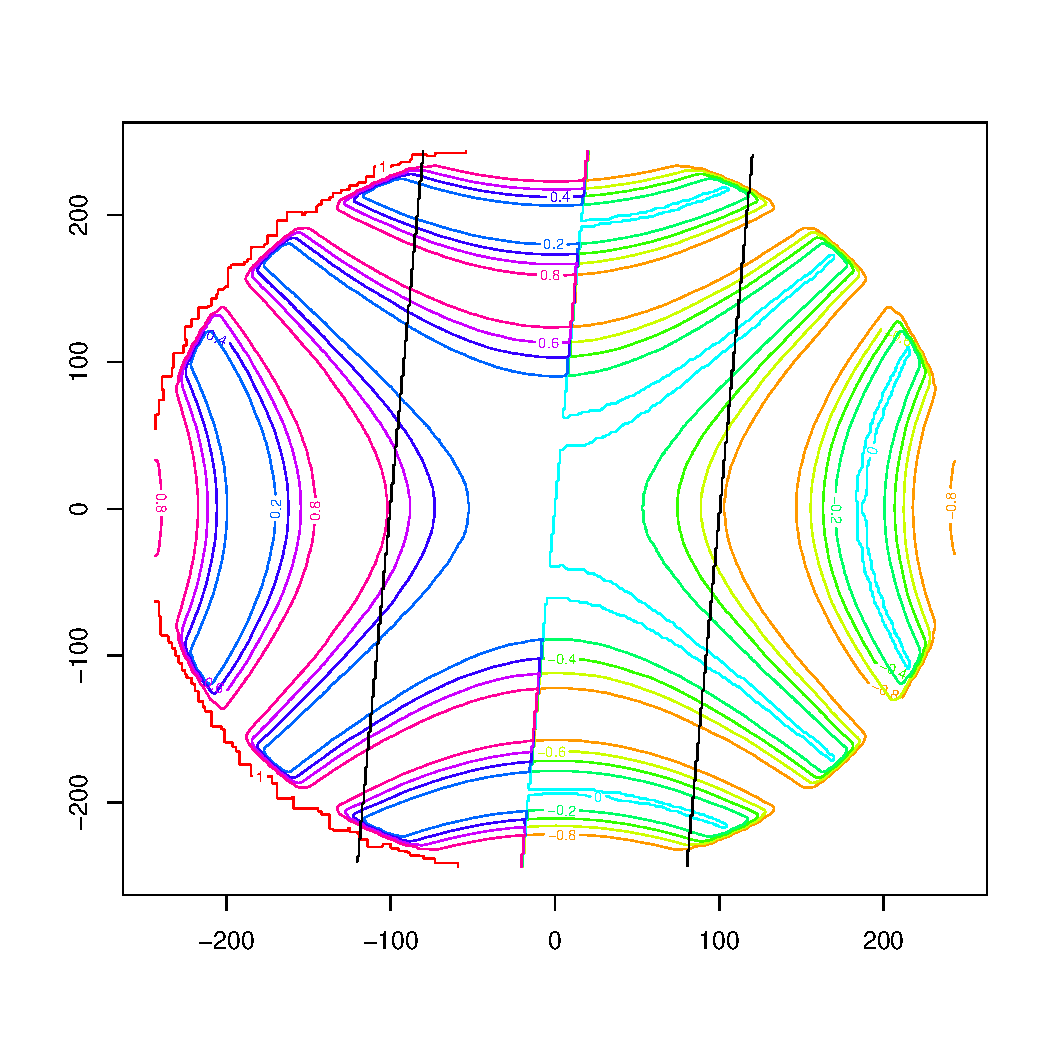
\includegraphics[width=0.3\textwidth]{Figures/conoscopy/1}}
\subfigure[Vertical]{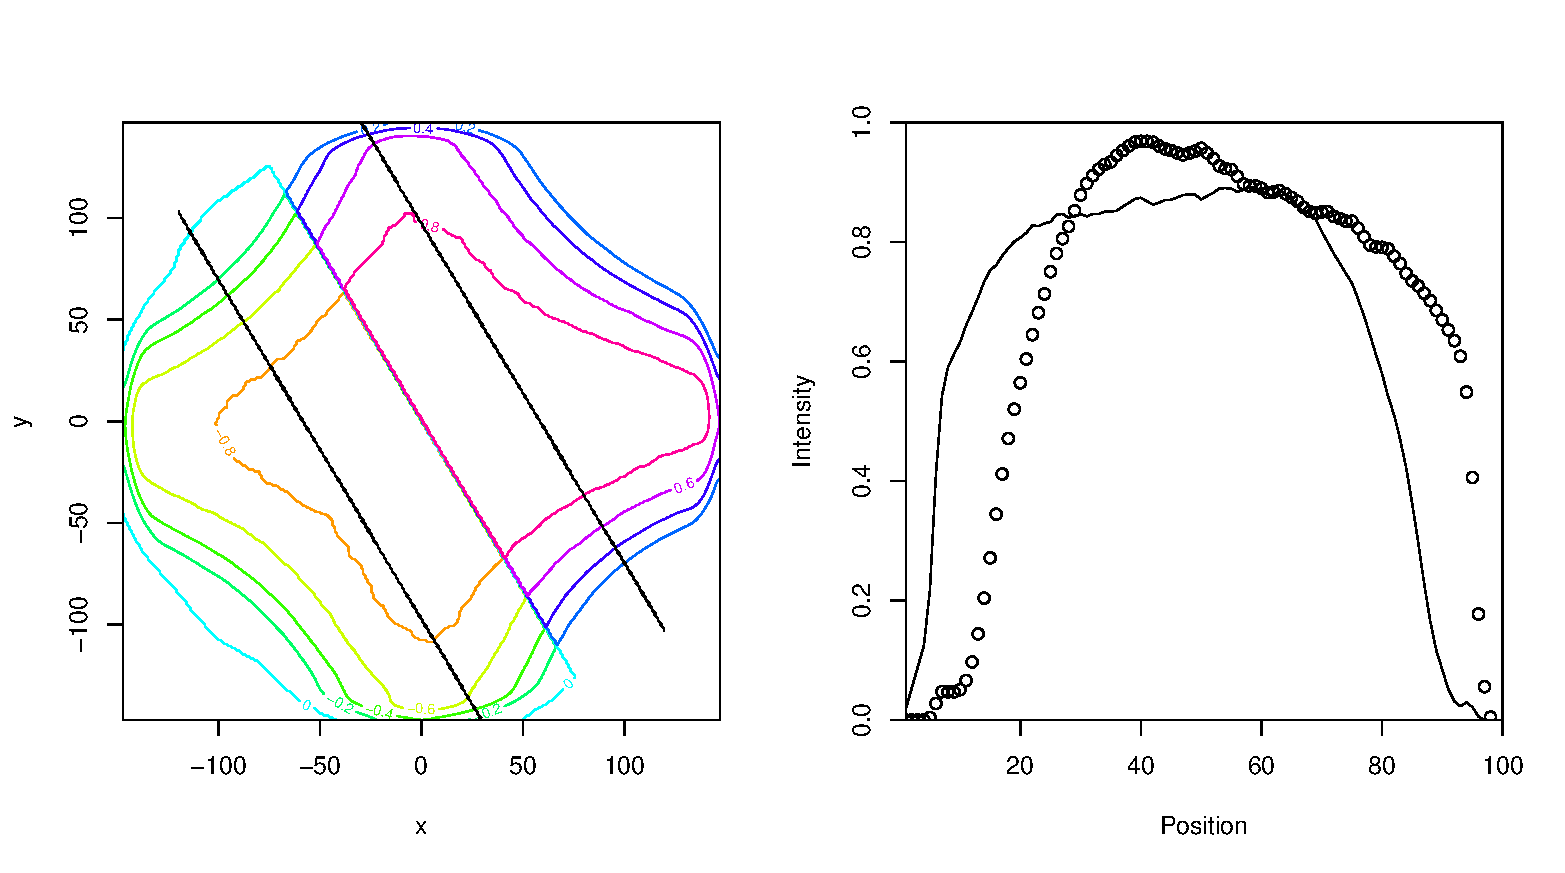
\includegraphics[width=0.3\textwidth]{Figures/conoscopy/2}}
\subfigure[Tilted]{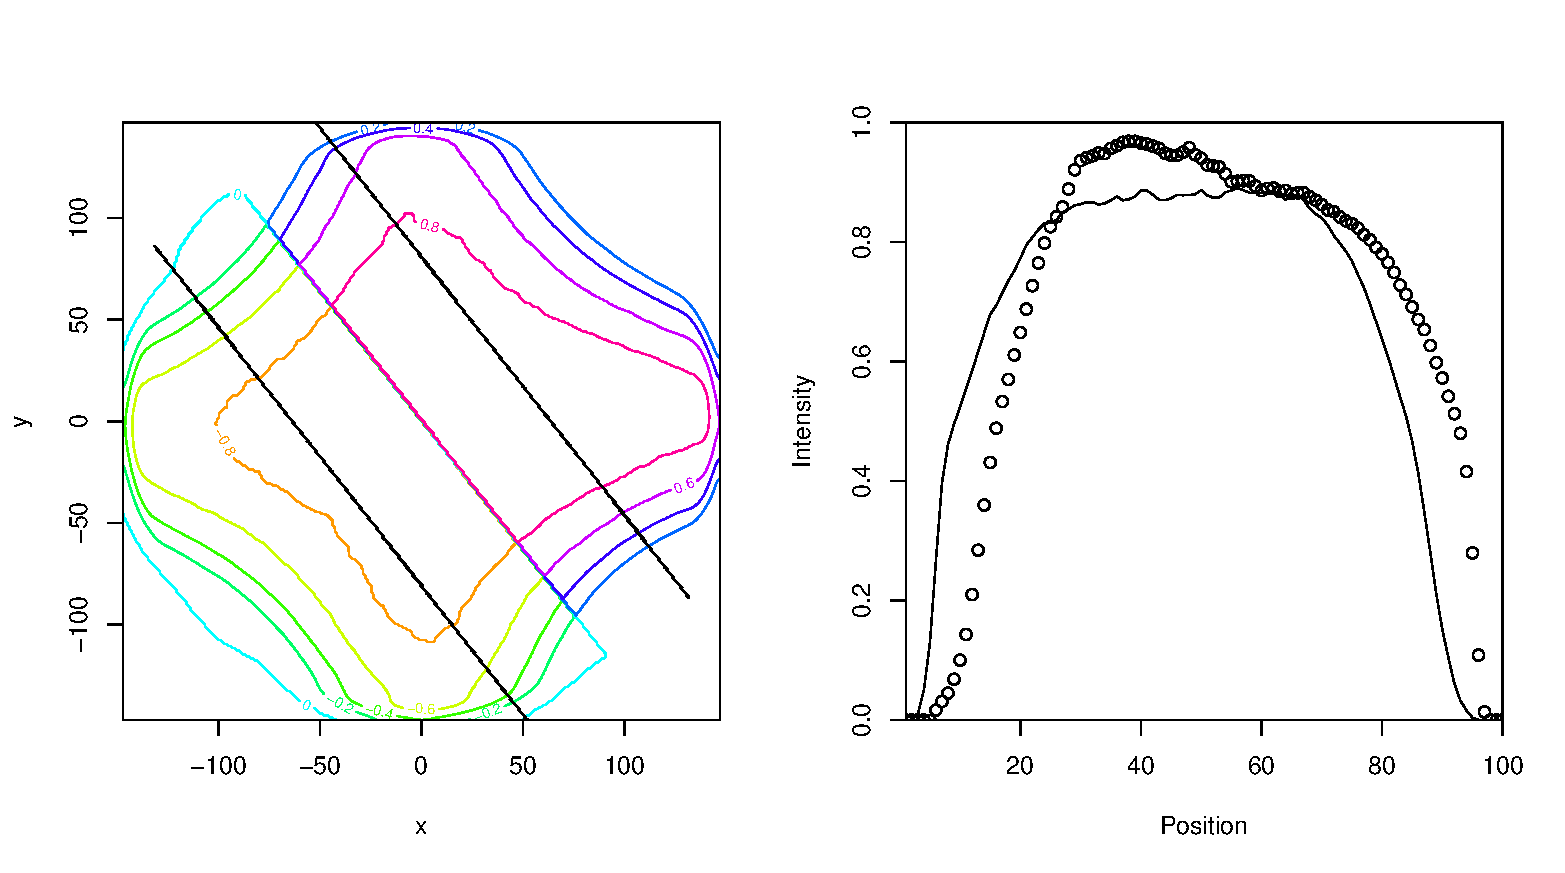
\includegraphics[width=0.3\textwidth]{Figures/conoscopy/3}}
\end{center}
\caption[Simulated conoscopic images for planar, vertical and tilted alignment]{\label{fig:con_samples}Simulated conoscopic figures for the director profiles shown schematically on the left. (a) the double set of hyperbolae signalling planar alignment. (b) The maltese cross from vertical alignment of the director. (c) A series of dark fringes from a uniformly tilted sample.}
\end{figure}

A modelling script was also developed by Stephen Cornford \cite{Cornford2008} in order to simulate the conoscopic figures observed for birefringent media. As used widely in his thesis, the Berreman \cite{Berreman1972} (or Jones) matrix methods were adapted to compute the conoscopic figures, as has been reported previously in the literature \cite{Ogasawara2001,Parry-Jones2002}.

Briefly, a cartesian coordinate system is defined for the computation of the conoscopic figure. Each point within that coordinate system $\left(x,y\right)$ can be defined by a pair of angles $\alpha$ and $\psi$ such that \cite{Cornford2008},

\begin{eqnarray}
\tan\psi=y/x\\
\sin\alpha=\left(x^2+y^2\right)^{\frac{1}{2}}
\end{eqnarray}

A ray of light that passes through the focus of the cone of light at an angle of incidence $\alpha$, strikes the cartesian coordinate system plane with a plane of incidence at angle $\psi$ to the figure's $x$ axis and at an angle $\psi^{\prime}$ to the transmission angle of the polariser. 

For each ray in the cone of incident light, the coefficients $E_{ss},E_{sp},E_{ps},E_{pp}$ are calculated, where $E_{sp}$ is the complex, $s$-polarised component of the electric field transmitted through the sample if the incoming ray were wholly $p$-polarised. From these, the intensity at any point on the cartesian coordinate system can be obtained \cite{Cornford2008} from,

\begin{align}
I\left(\alpha,\psi\right)=\left|\left(E_{pp}-E_{ps}\right)\sin\left(\psi^{\prime}\right)\cos\left(\psi^{\prime}\right)-E_{ps}\cos^2\psi^{\prime}+E_{sp}\sin^2\psi^{\prime}\right|^2
\end{align}

In order to compute the interference figure, a set of points in the cartesian coordinate plain $\left(x,y\right)$ needs to be selected such that $\sin\alpha\leq\sin\text{NA}$, where NA is the numerical aperture of the cone of light \cite{Cornford2008}.

Figure \ref{fig:figures} shows a table of simulated conoscopic figures from the computational method described above. These figures are simulated for a typical nematic liquid crystal with refractive indices of $n_e=1.7$ and $n_o=1.5$ in  a cell approximately 100 $\mu m$ thick. The sequence of figures correspond to the liquid crystal uniform tilt angle $\theta$ varying along a row, whilst the azimuthal angle $\phi$ varies along a column.

\begin{center}
\begin{table}[ht]
\newcolumntype{C}{>{\centering\arraybackslash} m{1cm}}
\begin{tabular}{ccCCCCC}
&&&&$\theta$&&\\
&&90$^{\circ}$&85$^{\circ}$&45$^{\circ}$&5$^{\circ}$&0$^{\circ}$\\
&\centering{90}$^{\circ}$&\includegraphics[width=0.06\textwidth]{Figures/conoscopy/table/90_90}&\includegraphics[width=0.06\textwidth]{Figures/conoscopy/table/90_85}&\includegraphics[width=0.06\textwidth]{Figures/conoscopy/table/90_45}&\includegraphics[width=0.06\textwidth]{Figures/conoscopy/table/90_05}&\includegraphics[width=0.06\textwidth]{Figures/conoscopy/table/90_00}\\

&60$^{\circ}$&\includegraphics[width=0.06\textwidth]{Figures/conoscopy/table/60_90}&\includegraphics[width=0.06\textwidth]{Figures/conoscopy/table/60_85}&\includegraphics[width=0.06\textwidth]{Figures/conoscopy/table/60_45}&\includegraphics[width=0.06\textwidth]{Figures/conoscopy/table/60_05}&\includegraphics[width=0.06\textwidth]{Figures/conoscopy/table/60_00}\\

$\phi$&45$^{\circ}$&\includegraphics[width=0.06\textwidth]{Figures/conoscopy/table/45_90}&\includegraphics[width=0.06\textwidth]{Figures/conoscopy/table/45_85}&\includegraphics[width=0.06\textwidth]{Figures/conoscopy/table/45_45}&\includegraphics[width=0.06\textwidth]{Figures/conoscopy/table/45_05}&\includegraphics[width=0.06\textwidth]{Figures/conoscopy/table/45_00}\\

&30$^{\circ}$&\includegraphics[width=0.06\textwidth]{Figures/conoscopy/table/30_90}&\includegraphics[width=0.06\textwidth]{Figures/conoscopy/table/30_85}&\includegraphics[width=0.06\textwidth]{Figures/conoscopy/table/30_45}&\includegraphics[width=0.06\textwidth]{Figures/conoscopy/table/30_05}&\includegraphics[width=0.06\textwidth]{Figures/conoscopy/table/30_00}\\

&0$^{\circ}$&\includegraphics[width=0.06\textwidth]{Figures/conoscopy/table/00_90}&\includegraphics[width=0.06\textwidth]{Figures/conoscopy/table/00_85}&\includegraphics[width=0.06\textwidth]{Figures/conoscopy/table/00_45}&\includegraphics[width=0.06\textwidth]{Figures/conoscopy/table/00_05}&\includegraphics[width=0.06\textwidth]{Figures/conoscopy/table/00_00}\\
\end{tabular}
\caption[Characteristic conoscopic figures]{\label{fig:figures}A table showing characteristic conoscopic figures for varying values of $\theta$ and $\phi$ from the optical simulation package. Note that the polarisers are set at $\phi+45^{\circ}$, otherwise some of the figures in the $\theta>0$ column would appear nearly or entirely black. This accounts for the rotation of the $\theta=0$ figure, which would be independent of $\phi$ if the polariser angle did not change.}
\end{table}
\end{center}

Here as expected, for planar alignment $\left(\theta=90^{\circ}\right)$, the conjugate set of hyperbolae centred on a common locus is computed. This set of hyperbolae is rotated as a function of the azimuthal alignment, $\phi$ relative to the figure's $x$ axis. For pure vertical alignment $\left(\theta=0^{\circ}\right)$, the concentric circular fringes and maltese cross are computed. As stated earlier, for small uniform tilt angles away from either planar or vertical alignment $\left(\theta=85^{\circ},5^{\circ}\right)$, the locus of the simulated conoscopic figure appears slightly displaced from the centre of the field of view along a line parallel to the plane containing the director azimuthal alignment angle $\phi$.

\subsection{Experimental}
Figure \ref{fig:conoscope_schem} is a schematic diagram of the experimental set up that constitutes the conoscope used for analysis in this thesis. Here it is seen that firstly, light from a Helium-Neon laser (633 nm) is incident onto a rotating diffuser, acting as a scattering near point source over the small area illuminated by the beam spot. As the diffuser is rotated, the array of point sources varies, and when averaged over a single rotation of the diffuser, creates a uniform cone of light, removing any speckle pattern from the laser and final conoscopic figures. The beam is then collimated before passing through the first polariser and into the first microscope objective of the main assembly.

%\begin{figure}
%\begin{center}
%\subfigure[Experimental conoscope setup]{\includegraphics[width=\textwidth]{Figures/conoscopy/conoscope_setup}}\vspace{1cm}
%\subfigure[Magnification of cell in beam]{\includegraphics[width=0.6\textwidth]{Figures/Theory/cell_cono}}
%\end{center}
%\caption{\label{fig:conoscope_schem}(a)A schematic diagram of the conoscope used in this research. Based on a designs from the literature \cite{Parry-Jones2002,Fujikawa1993} and built by Cornford in reference \cite{Cornford2008}. Here, a collimated beam passes through the polariser, main assembly and sample, before passing through the analyser and focussed on to the CCD to capture a figure. (b) A magnification of a characteristic liquid crystal flow cell in the main assembly.}
%\end{figure}

\begin{figure}
\begin{center}
\includegraphics[width=0.48\textwidth]{Figures/conoscopy/conoscope_setup}
\end{center}
\caption[Schematic diagram of the conoscope setup]{\label{fig:conoscope_schem}A schematic diagram of the conoscope used in this research. Based on a designs from the literature \cite{Parry-Jones2002,Fujikawa1993} and built by Cornford in reference \cite{Cornford2008}. Here, a collimated beam passes through the polariser, main assembly and sample, before passing through the analyser and focussed on to the CCD to capture a figure.}
\end{figure}

The main assembly consists of the sample and two Mitotouyo Plan-Apo 50$\times$ long working distance microscope objectives. The first objective takes a parallel beam of light about 3 mm in diameter, expands it, and focusses it on to the sample. The resulting convergent beam has a numerical aperture of 0.55, and a working distance of 13 mm. Having passed through the sample, the second objective collimates the beam before it passes through the second polariser, also known as the analyser.

Finally, the beam passes through a correcting lens to correct for the change in focus of the convergent beam that is generated by passing through the two thick glass plates of the sample. When the outer part of the beam exiting the second objective is parallel, the inner part is convergent (clearly visible as the beam is brighter in the centre than at the edges). On going through the correcting lens, the beam is uniform in a single plane, and that is the position where the CCD is placed \cite{Cornford2008}, creating a conoscopic figure which is captured from computer software for the camera used.

The following sub-sections will look at sample data images captured from the conoscope shown schematically in Figure \ref{fig:conoscope_schem}. It will show (primarily for planar aligned samples) how the conoscopic figures respond to variations in certain parameters of the experimental setup, such as rotating the samples in the main assembly and rotating the polariser and analyser whilst viewing the conoscopic figure. These figures are compared to the computed figures from the optical simulation in order to confirm that the model is behaving accurately in predicting the correct conoscopic figure. Whilst the main focus of the work in this chapter, and in this thesis as a whole, is concerned with planar and near-planar aligned samples, some vertically aligned samples are included here in order to show the characteristic conoscopic figures that can be obtained.

\subsection{Planar alignment - rotating the cell}
All planar conoscopic images included in the following sections are taken from the same liquid crystal cell which is filled with 5CB sandwiched between two glass plates spaced with un-stretched Parafilm (thickness of approximately 100 $\mu m$). The surface alignment layer is a rubbed polyimide. For all simulation, refractive indices for 5CB at a wavelength of 633 nm and 25 $^{\circ}$C are used as $n_o=1.531$ and $n_e=1.706$ taken from reference \cite{Li2005}.

Firstly, Figure \ref{fig:rotate_cell_data} shows how the planar conoscopic figure responds when the cell is physically rotated when in the conoscope. Here the polariser and analyser remain crossed at $0^\circ$ and $90^\circ$ to the image's $x$ axis whilst the cell is rotated in increments of approximately $5^\circ$. The rubbing direction is initially at $45^\circ$ to the figure's $x$ axis (Figure \ref{fig:rotate_cell_data} (a)). As the cell is rotated, the conjugate hyperbolae that make the conoscopic figure, clearly rotate until the rubbing direction becomes parallel to the polariser direction. In this position, the incident light sees only one refractive index of the liquid crystal, resulting in no average polarisation conversion of the incident light. As such, all rays arriving at the analyser are stopped and the field of view becomes completely dark (Figure \ref{fig:rotate_cell_data} (i)). The same effect is also seen when the rubbing direction is exactly perpendicular to the polariser. If the cell were to be rotated through $360^\circ$, this field of view will go dark four times in total, that is, whenever the director is parallel to either the polariser or analyser.

\begin{figure}
\begin{center}
\subfigure[]{\includegraphics[width=0.1\textwidth]{Figures/conoscopy/Rotate_cell/00.jpg}}
\subfigure[]{\includegraphics[width=0.1\textwidth]{Figures/conoscopy/Rotate_cell/01.jpg}}
\subfigure[]{\includegraphics[width=0.1\textwidth]{Figures/conoscopy/Rotate_cell/02.jpg}}
\subfigure[]{\includegraphics[width=0.1\textwidth]{Figures/conoscopy/Rotate_cell/03.jpg}}
\subfigure[]{\includegraphics[width=0.1\textwidth]{Figures/conoscopy/Rotate_cell/04.jpg}}
\subfigure[]{\includegraphics[width=0.1\textwidth]{Figures/conoscopy/Rotate_cell/05.jpg}}
\subfigure[]{\includegraphics[width=0.1\textwidth]{Figures/conoscopy/Rotate_cell/06.jpg}}
\subfigure[]{\includegraphics[width=0.1\textwidth]{Figures/conoscopy/Rotate_cell/07.jpg}}
\subfigure[]{\includegraphics[width=0.1\textwidth]{Figures/conoscopy/Rotate_cell/08.jpg}}
\subfigure[]{\includegraphics[width=0.1\textwidth]{Figures/conoscopy/Rotate_cell/09.jpg}}
\subfigure[]{\includegraphics[width=0.1\textwidth]{Figures/conoscopy/Rotate_cell/10.jpg}}
\subfigure[]{\includegraphics[width=0.1\textwidth]{Figures/conoscopy/Rotate_cell/11.jpg}}
\subfigure[]{\includegraphics[width=0.1\textwidth]{Figures/conoscopy/Rotate_cell/12.jpg}}
\subfigure[]{\includegraphics[width=0.1\textwidth]{Figures/conoscopy/Rotate_cell/13.jpg}}
\subfigure[]{\includegraphics[width=0.1\textwidth]{Figures/conoscopy/Rotate_cell/14.jpg}}
\subfigure[]{\includegraphics[width=0.1\textwidth]{Figures/conoscopy/Rotate_cell/15.jpg}}
\subfigure[]{\includegraphics[width=0.1\textwidth]{Figures/conoscopy/Rotate_cell/16.jpg}}
\subfigure[]{\includegraphics[width=0.1\textwidth]{Figures/conoscopy/Rotate_cell/17.jpg}}
%\subfigure[]{\includegraphics[width=0.15\textwidth]{Figures/conoscopy/Rotate_cell/18.jpg}}
\end{center}
\caption[Conoscopic images of a planar cell - rotating]{\label{fig:rotate_cell_data}Data conoscopic figures for a planar aligned cell. The polariser and analyser remain crossed at $0^\circ$ and $90^\circ$ to the figure's $x$ axis whilst the cell is rotated in increments of approximately $5^\circ$ through images (a) to (r). When the cell is rotated so that the rubbing direction becomes parallel to either the polariser or analyser (image (i)), the field of view is shown to be  completely dark. This is due to the incident light experiencing only one of the refractive indices of the liquid crystal, resulting in no polarisation conversion and all light being blocked by the analyser.}
\end{figure}

Figure \ref{fig:rotate_cell_model} now shows the simulated conoscopic figures for the same experimental setup from which the conoscopic figures in Figure \ref{fig:rotate_cell_data} were obtained. This has been achieved by simulating the director profile to be aligned at varying azimuthal angles, whilst maintaining the polariser and analyser at $0^\circ$ and $90^\circ$ degrees respectively. It is clear that the uniaxial optics simulation provides very good agreement with the data obtained from the actual conoscope. As the azimuthal alignment of the director is changed, the field of view goes from showing the conjugate set of hyperbolae to going completely dark when the director and polariser or analyser are parallel with one another (Figure \ref{fig:rotate_cell_model} (i)).
 
\begin{figure}
\begin{center}
\subfigure[]{\includegraphics[width=0.1\textwidth]{Figures/conoscopy/Rotate_cell/modelled/cropped/01.jpg}}
\subfigure[]{\includegraphics[width=0.1\textwidth]{Figures/conoscopy/Rotate_cell/modelled/cropped/02.jpg}}
\subfigure[]{\includegraphics[width=0.1\textwidth]{Figures/conoscopy/Rotate_cell/modelled/cropped/03.jpg}}
\subfigure[]{\includegraphics[width=0.1\textwidth]{Figures/conoscopy/Rotate_cell/modelled/cropped/04.jpg}}
\subfigure[]{\includegraphics[width=0.1\textwidth]{Figures/conoscopy/Rotate_cell/modelled/cropped/05.jpg}}
\subfigure[]{\includegraphics[width=0.1\textwidth]{Figures/conoscopy/Rotate_cell/modelled/cropped/06.jpg}}
\subfigure[]{\includegraphics[width=0.1\textwidth]{Figures/conoscopy/Rotate_cell/modelled/cropped/07.jpg}}
\subfigure[]{\includegraphics[width=0.1\textwidth]{Figures/conoscopy/Rotate_cell/modelled/cropped/08.jpg}}
\subfigure[]{\includegraphics[width=0.1\textwidth]{Figures/conoscopy/Rotate_cell/modelled/cropped/09.jpg}}
\subfigure[]{\includegraphics[width=0.1\textwidth]{Figures/conoscopy/Rotate_cell/modelled/cropped/10.jpg}}
\subfigure[]{\includegraphics[width=0.1\textwidth]{Figures/conoscopy/Rotate_cell/modelled/cropped/11.jpg}}
\subfigure[]{\includegraphics[width=0.1\textwidth]{Figures/conoscopy/Rotate_cell/modelled/cropped/12.jpg}}
\subfigure[]{\includegraphics[width=0.1\textwidth]{Figures/conoscopy/Rotate_cell/modelled/cropped/13.jpg}}
\subfigure[]{\includegraphics[width=0.1\textwidth]{Figures/conoscopy/Rotate_cell/modelled/cropped/14.jpg}}
\subfigure[]{\includegraphics[width=0.1\textwidth]{Figures/conoscopy/Rotate_cell/modelled/cropped/15.jpg}}
\subfigure[]{\includegraphics[width=0.1\textwidth]{Figures/conoscopy/Rotate_cell/modelled/cropped/16.jpg}}
\subfigure[]{\includegraphics[width=0.1\textwidth]{Figures/conoscopy/Rotate_cell/modelled/cropped/17.jpg}}
\subfigure[]{\includegraphics[width=0.1\textwidth]{Figures/conoscopy/Rotate_cell/modelled/cropped/18.jpg}}
%\subfigure[]{\includegraphics[width=0.15\textwidth]{Figures/conoscopy/Rotate_cell/18.jpg}}
\end{center}
\caption[Simulated conoscopic images of a planar cell - rotating]{\label{fig:rotate_cell_model}Simulated conoscopic figures as the director azimuthal alignment is rotated in increments of $5^\circ$ from (a) to (r). These figures can be directly compared to the data conoscopic figures shown in Figure \ref{fig:rotate_cell_data} where a good agreement is seen.}
\end{figure}

\subsection{Planar alignment - rotating the polarisers}
A second experiment was also carried out, in which the cell was maintained in the same orientation (director at $45^\circ$ to the image's $x$ axis) but now, the polariser and analyser were rotated in $10^\circ$ increments whilst always remaining at $90^\circ$ to one another (crossed). The conoscopic figures obtained can be seen in Figure \ref{fig:stationary_cell_data}, images (a) to (j). As expected, the conjugate hyperbolae which make up the conoscopic figure remain undistorted, whilst the field of view gets darker before becoming completely black when either the polariser or analyser are aligned parallel to the rubbing direction (f). As the polariser and analyser are rotated past being parallel to the rubbing direction, the field of view becomes brighter again, returning to the initial conoscopic figure.

\begin{figure}
\begin{center}
\subfigure[]{\includegraphics[width=0.1\textwidth]{Figures/conoscopy/Stationary_cell/00.jpg}}
\subfigure[]{\includegraphics[width=0.1\textwidth]{Figures/conoscopy/Stationary_cell/01.jpg}}
\subfigure[]{\includegraphics[width=0.1\textwidth]{Figures/conoscopy/Stationary_cell/02.jpg}}
\subfigure[]{\includegraphics[width=0.1\textwidth]{Figures/conoscopy/Stationary_cell/03.jpg}}
\subfigure[]{\includegraphics[width=0.1\textwidth]{Figures/conoscopy/Stationary_cell/04.jpg}}
\subfigure[]{\includegraphics[width=0.1\textwidth]{Figures/conoscopy/Stationary_cell/05.jpg}}
\subfigure[]{\includegraphics[width=0.1\textwidth]{Figures/conoscopy/Stationary_cell/06.jpg}}
\subfigure[]{\includegraphics[width=0.1\textwidth]{Figures/conoscopy/Stationary_cell/07.jpg}}
\subfigure[]{\includegraphics[width=0.1\textwidth]{Figures/conoscopy/Stationary_cell/08.jpg}}
\subfigure[]{\includegraphics[width=0.1\textwidth]{Figures/conoscopy/Stationary_cell/09.jpg}}
\end{center}
\caption[Conoscopic images of a planar cell - rotating polarisers]{\label{fig:stationary_cell_data}Planar cell with the rubbing direction at at $45^\circ$ to the $x$ axis. The polariser and analyser remain crossed to one another whilst they are rotated in approximately $10^\circ$ increments from (a) to (j)}
\end{figure}

Figure \ref{fig:stationary_cell_model} again shows the simulated conoscopic figures for the same experimental set up, in which the alignment angle in the cell remains constant, and the polariser and analyser are rotated in $10^\circ$ increments whilst always remaining crossed to one another. Here again, it is clear that the uniaxial optics simulation provides very good agreement with the data obtained from the conoscope. As the polariser and analyser are rotated, the field of view goes from showing the conjugate set of hyperbolae to appearing completely dark when the director and polariser or analyser are parallel with each other (Figure \ref{fig:stationary_cell_model} (f)).

\begin{figure}
\begin{center}
\subfigure[]{\includegraphics[width=0.1\textwidth]{Figures/conoscopy/Stationary_cell/modelled/cropped/00.jpg}}
\subfigure[]{\includegraphics[width=0.1\textwidth]{Figures/conoscopy/Stationary_cell/modelled/cropped/01.jpg}}
\subfigure[]{\includegraphics[width=0.1\textwidth]{Figures/conoscopy/Stationary_cell/modelled/cropped/02.jpg}}
\subfigure[]{\includegraphics[width=0.1\textwidth]{Figures/conoscopy/Stationary_cell/modelled/cropped/03.jpg}}
\subfigure[]{\includegraphics[width=0.1\textwidth]{Figures/conoscopy/Stationary_cell/modelled/cropped/04.jpg}}
\subfigure[]{\includegraphics[width=0.1\textwidth]{Figures/conoscopy/Stationary_cell/modelled/cropped/05.jpg}}
\subfigure[]{\includegraphics[width=0.1\textwidth]{Figures/conoscopy/Stationary_cell/modelled/cropped/06.jpg}}
\subfigure[]{\includegraphics[width=0.1\textwidth]{Figures/conoscopy/Stationary_cell/modelled/cropped/07.jpg}}
\subfigure[]{\includegraphics[width=0.1\textwidth]{Figures/conoscopy/Stationary_cell/modelled/cropped/08.jpg}}
\subfigure[]{\includegraphics[width=0.1\textwidth]{Figures/conoscopy/Stationary_cell/modelled/cropped/09.jpg}}
\end{center}
\caption[Simulated conoscopic images of a planar cell - rotating polarisers]{\label{fig:stationary_cell_model}Simulated conoscopic figures whereby the polariser and analyser remain crossed to one another and are rotated in increments of $10^\circ$ from (a) to (j). These figures can be directly compared to the data conoscopic figures shown in Figure \ref{fig:stationary_cell_data} whereby a good agreement is seen.}
\end{figure}

\subsection{Planar alignment - thickness variation}
Figure \ref{fig:planar_thickness} demonstrates how the planar alignment conoscopic figure varies as a function of the cell thickness. The conoscopic figures in Figure \ref{fig:planar_thickness} were achieved by tracking across the cell in the $x-y$ plane with each image (a) to (g) taken at a different point. Here it is shown that the conjugate set of hyperbolae can move into and out of the centre of the conoscopic figure. As the cell thickness increases, there will be more fringes visible within the field of view. Conversely, as the cell thickness decreases, there will be fewer fringes in the field of view. This effect of cell thickness on fringe number is also true in the case of a vertically aligned sample (shown later in Figure \ref{fig:homeotropic_cell}), where extra sets of concentric circular fringes can be seen as the cell thickness increases. In Figure \ref{fig:planar_thickness}, the director is aligned at 45$^\circ$ to the figure's $x$ axis, and most importantly, there is very little change in this angle of orientation as the cell is moved around. This demonstrates that the rubbed polymer alignment layer has produced spatially coherent director alignment over a relatively large area (millimetres) of the cell. 

\begin{figure}
\begin{center}
\subfigure[]{\includegraphics[width=0.1\textwidth]{Figures/conoscopy/Planar_thickness/0}}
\subfigure[]{\includegraphics[width=0.1\textwidth]{Figures/conoscopy/Planar_thickness/1.jpg}}
\subfigure[]{\includegraphics[width=0.1\textwidth]{Figures/conoscopy/Planar_thickness/2.jpg}}
\subfigure[]{\includegraphics[width=0.1\textwidth]{Figures/conoscopy/Planar_thickness/3.jpg}}
\subfigure[]{\includegraphics[width=0.1\textwidth]{Figures/conoscopy/Planar_thickness/4.jpg}}
\subfigure[]{\includegraphics[width=0.1\textwidth]{Figures/conoscopy/Planar_thickness/5.jpg}}
\subfigure[]{\includegraphics[width=0.1\textwidth]{Figures/conoscopy/Planar_thickness/6.jpg}}
\end{center}
\caption[Conoscopic images of thickness variations in a planar cell]{\label{fig:planar_thickness}Conoscopic interference figure for a planar cell rubbed at 45$^\circ$ to the figure's $x$ axis. Polariser and analyser are crossed and at 0$^\circ$ and 90$^\circ$ to the figure's $x$ axis. Figures (a) through (g) show how the figure changes when moving the cell approximately 5 mm in the x-direction due to a depth gradient across the cell.}
\begin{center}
%\rule{3in}{0.5pt}
\end{center}
\end{figure}

\subsection{Vertical alignment}
Figure \ref{fig:homeotropic_cell} shows captured conoscopic figures for a cell that has been aligned vertically through a surface treatment of lecithin dissolved in ether\footnote{In order to achieve a good alignment layer, a small amount of lecithin is dissolved in the ether until the solution becomes pale yellow in colour. The face is then coated by dragging a lens tissue soaked in the solution across the glass surface.}. Here it is shown that the conoscopic figure consists of (as described earlier) concentric circular fringes and a central extinction cross that is often referred to as the `classic' maltese cross. Figure \ref{fig:homeotropic_cell} (a) and (b) show captured conoscopic figures for the same vertically aligned cell whereby the polariser and analyser are crossed $0^\circ$ and $90^\circ$ to the $x$ axis, and at $45^\circ$ and $135^\circ$ to the $x$ axis respectively. This difference in polariser/analyser alignment is shown by the rotation of the extinction cross through $45^\circ$. Figures \ref{fig:homeotropic_cell} (c) and (d) show two conoscopic figure captures from a different cell, in which a thickness gradient exists. Much like in the case of the planar conoscopic figure example (Figure \ref{fig:planar_thickness}) the number of concentric circular fringes visible at the edge of the field of view increases as the cell becomes thicker. This is visible when looking at image (c) with just one set of fringes and image (d) which contains two sets of fringes\footnote{The slight displacement of the locus from the centre of the field of view in Figure \ref{fig:homeotropic_cell} (c) and (d) when compared with (a) and (b) suggests that the director may be slightly tilted away from vertical alignment}.


\begin{figure}
\begin{center}
\subfigure[]{\includegraphics[width=0.1\textwidth]{Figures/conoscopy/homeotropic/00.jpg}}
\subfigure[]{\includegraphics[width=0.1\textwidth]{Figures/conoscopy/homeotropic/01.jpg}}\\
\subfigure[]{\includegraphics[width=0.1\textwidth]{Figures/conoscopy/homeotropic/03.jpg}}
\subfigure[]{\includegraphics[width=0.1\textwidth]{Figures/conoscopy/homeotropic/04.jpg}}
\end{center}
\caption[Conoscopic figures from a vertically aligned cell]{\label{fig:homeotropic_cell}Data conoscopic figure captures of a a cell aligned vertically through a surface treatment of lecithin dissolved in ether. Figures (a) and (b) show figures where the crossed polarisers are at $0^{\circ}$ and $45^{\circ}$ to the $x$ axis respectively. Figures (c) and (d) depict a vertically aligned cell whereby (d) is captured in a slightly thicker part of the cell, with more fringes visible around the maltese cross.}
\end{figure}

\subsection{Polarisers crossed and parallel}
Finally, Figure \ref{fig:pol_crossed_parallel} shows a comparison between planar aligned and vertically aligned captured conoscopic figures viewed when the polariser and analyser are crossed to one another (a) and (c) and also when the analyser has been rotated to become parallel to the polariser (b) and (d). These figures were again captured as a test to see whether the conoscope was working as expected. For both cases, the conoscopic figures captured when the polariser and analyser are parallel to one another appear to be the inverse of the figures where the polariser and analyser are crossed to one another. This is as expected. When the analyser is rotated to be parallel to the polariser, any light that exits the cell polarised orthogonal to the analyser will be blocked, resulting in a dark area on the conoscopic figure. When the analyser is rotated through $90^{\circ}$ to be parallel to the polariser, this same light will be passed by the analyser, resulting in a light area on the conoscopic figure. This is shown by Figure \ref{fig:pol_crossed_parallel} (b) now having a dark centre, and most strikingly the inverse vertically aligned conoscopic figure whereby a light cross is formed by four dark lobes.

\begin{figure}
\begin{center}
\subfigure[]{\includegraphics[width=0.1\textwidth]{Figures/conoscopy/polarisers/00.jpg}}
\subfigure[]{\includegraphics[width=0.1\textwidth]{Figures/conoscopy/polarisers/01.jpg}}\\
\subfigure[]{\includegraphics[width=0.1\textwidth]{Figures/conoscopy/polarisers/02.jpg}}
\subfigure[]{\includegraphics[width=0.1\textwidth]{Figures/conoscopy/polarisers/03.jpg}}
\end{center}
\caption[Conoscopic images when polarisers are crossed and parallel]{\label{fig:pol_crossed_parallel}A comparison between data conoscopic figures for a planar aligned cell and a vertically aligned cell viewed when the polariser and analyser are crossed to one another and also when they are parallel to one another. Images (a) and (b) show a planar aligned cell viewed conoscopically between crossed and parallel polarisers respectively. Images (c) and (d) show a vertically aligned cell viewed conoscopically between crossed and parallel polarisers respectively. In both cases, the conoscopic figures are essentially the inverse of the original.}
\end{figure}

\subsection{Tracking conoscopic figure alignment}
In order to accurately determine the alignment angle of the conjugate hyperbolae present in the planar conoscopic figure, a computer minimisation routine was created to automatically iterate down to the correct angle. Typical output figures from this program can be seen in Figure \ref{fig:figure_rotation1}. Before the automated routine can be run, the conoscopic figures must be lightly processed in order for them to work with the computer program. This processing involves cropping the images to be square, and smoothing the figures to remove any artefacts that may give misleading results (simple gaussian smoothing in ImageJ is suitable for this). Examples of an original simulated planar conoscopic figure and the smoothed version can be seen in Figure \ref{fig:figure_rotation1} (a) and (b). 

In order to accurately determine the angle at which the hyperbolae are aligned, the program plots an initial line running through the centre of the field of view at a pre-defined angle (normally measured from the $x$ axis of the figure). Two further test lines are then plotted parallel and at a fixed distance to the initial line. The automated routine then plots the values of the pixel intensities along these two test lines and plots them as a function of position along the test line. Pairs of images can be seen in Figure \ref{fig:figure_rotation1} (c) to (j) in which the test lines plotted on the conoscopic figure (left column) correspond to the pixel intensities as a function of position on the line (plotted in the right column). The program then alters the angle at which the initial line is plotted (each time re-plotting two new parallel test lines) and measuring the difference between the pixel intensities for this given initial line. The automated routine varies the initial line angle to iterate down to a line which best minimises the difference in sum of the pixel intensities between the two test lines. At this point, the angle of the plotted line defines the angle at which the conjugate hyperbolae of the conoscopic figure are aligned.

For example, Figure \ref{fig:figure_rotation1} (c) shows the initial line and the two test lines plotted either side for the first iteration. It is clear by eye that the initial guess does not minimise the difference in pixel intensities of the two lines, although this is confirmed in (d) whereby the pixel intensities along the test lines in image (c) are plotted. It is clearly visible that the data points and line do not overlap each other. The second iteration (images (e) and (f)) make the situation even worse, with a bigger difference between the plotted pixel intensities. Accordingly, the third iteration moves the test line in the opposite direction ((g) and (h)) and a smaller difference between the test line pixel intensities is found. After the fourth iteration, the difference between the test line pixel intensities is minimised ((i) and (j)) and the angle at which the test lines are plotted over the conoscopic figure is returned by the program. In practice, this process may take more than four iterations, but is a valuable tool in systematically and automatically ascertaining the alignment angle of the conjugate hyperbolae of the planar conoscopic figure.

As will be seen in later chapters, the fits between the plotted pixel intensities are far worse when the automated routine is carried out on actual conoscopic figures as opposed to here where the simulated noise-free figures provide easy minimisation and near perfect evaluation of the alignment angle.

\begin{figure}
\begin{center}
\subfigure[Original]{\includegraphics[width=0.15\textwidth]{Figures/Mirror/bob}}\hspace{0.4cm}
\subfigure[Smoothed]{\includegraphics[width=0.15\textwidth]{Figures/Mirror/bobsmooth}}\\
\scalebox{0.9}[1]{\subfigure[]{\includegraphics[width=0.2\textwidth]{Figures/Mirror/1}}}
\scalebox{0.9}[1]{\subfigure[]{\includegraphics[width=0.2\textwidth]{Figures/Mirror/2}}}\\
\scalebox{0.9}[1]{\subfigure[]{\includegraphics[width=0.2\textwidth]{Figures/Mirror/3}}}
\scalebox{0.9}[1]{\subfigure[]{\includegraphics[width=0.2\textwidth]{Figures/Mirror/4}}}\\
\scalebox{0.9}[1]{\subfigure[]{\includegraphics[width=0.2\textwidth]{Figures/Mirror/5}}}
\scalebox{0.9}[1]{\subfigure[]{\includegraphics[width=0.2\textwidth]{Figures/Mirror/6}}}\\
\scalebox{0.9}[1]{\subfigure[]{\includegraphics[width=0.2\textwidth]{Figures/Mirror/9}}}
\scalebox{0.9}[1]{\subfigure[]{\includegraphics[width=0.2\textwidth]{Figures/Mirror/10}}}
\end{center}
\caption[Automated conoscopic figure tracking routine]{\label{fig:figure_rotation1}(a) Original simulated conoscopic figure. (b) Original figure after smoothing in ImageJ. Images (c) to (j) show pairs of images whereby the pixel intensities plotted along the two lines either side of the central test line are plotted. After three iterations, the difference between the left and right test lines has been minimised resulting in determination of the azimuthal alignment angle of the conoscopic figure.}
\end{figure}

This chapter will now go on to discuss the cell fabrication methods developed during this study in order to conduct the pressure driven flow experiments that will be detailed in the following chapters.

\subsection{Cell fabrication}
\label{sec:cell_fabrication}
In order to conduct dynamic pressure driven flow experiments, robust cells that allow flow of a liquid crystal from a syringe drive must be fabricated. During the course of this investigation, a set technique has been developed, refined and improved upon, to become what is now a standard process for the production of pressure driven flow cells within the group at Exeter.

Cells are generally constructed from a standard glass microscope slide that has been cut in half to produce two approximately 3 cm by 2 cm plates. One of the plates is drilled with holes by our workshop technicians to allow for the inlet/outlet pipes to be attached. The plates are then cleaned (see below), before having a surface alignment layer deposited, and rubbed if necessary.

\subsection{Microscope slide preparation}
\begin{enumerate}
\item 
All cleaning of microscope slides and cover slips is carried out in clean tents, where fans perpetually circulate the air in the immediate environment. All processes are also carried out wearing latex gloves to minimise contamination with skin grease or other foreign bodies from the immediate environment.
\item 
Slides are removed from their sealed container and firstly cleaned rigorously with a cotton bud soaked in acetone. Initially they are rubbed with firm pressure in one direction and then rubbed again at 90$^{\circ}$ to the initial cleaning direction. This technique is considered to be a mechanical cleaning process to get rid of any debris or small particles that may be on the surface of the slide. The acetone also aids in removing any grease or smudges that are present on the slides\footnote{One must take care not to use the same end of the cotton bud twice as this can result in contamination of the solvent reservoir}.
\item 
Step 2 is then repeated with cotton buds soaked in isopropanol (IPA). This step removes any residue left by the acetone on the surface of the slide. The slides are then blasted with an inert dusting gas to remove any fibres that may have been left by the cotton buds.
\item 
Finally, and most importantly, the slides are drag cleaned with lens tissue soaked in IPA. The lens tissue is placed over the slide and pulled slowly (at approximately the same rate that the IPA evaporates) across the slide with tweezers. This process removes any smears or debris left by the previous stages. This step can be repeated several times until the slide is free of any defects when examined by eye.
\end{enumerate}

\subsection{Cell construction}
\label{sec:cell_construction}
At this stage, aligning layers can be deposited onto the glass slides. Conventionally this is done by spin coating a layer of polyimide in order to align the director, whereby the particular composition of the polymer promotes a particular alignment. Once the glass slides have been prepared with an alignment layer, they are ready to be brought together to form a flow cell. Figure \ref{fig:cell_fabrication} shows a schematic diagram of this process. 

\begin{figure}
\begin{center}
\includegraphics[width=0.49\textwidth]{Figures/45/cell_fabrication}
\end{center}
\caption[Cell fabrication]{\label{fig:cell_fabrication}(a) The glass slides are placed on a clean and flat surface ready for cell construction. (b) Stretched strips of \textit{Parafilm} are placed either side of the inlet/outlet holes to define a flow channel. (c) The plates are sandwiched together and the excess \textit{Parafilm} is removed. The cell is then placed on a hot plate to bond the  \textit{Parafilm} to the glass. (d) UV curing glue is introduced to seal the channel ends and cured under a UV lamp. (e) Inlet and outlet pipes are attached to the flow cell with an epoxy resin adhesive.}
\end{figure}

\begin{enumerate}
\item 
Firstly, the slides are placed on a flat clean surface and arranged so that the top plate can be placed on top of the bottom plate to create the initial alignment conditions required.
\item
Two thin strips of \textit{Parafilm} are cut and stretched by hand to form the walls of the flow channel. Prior to stretching, the \textit{Parafilm} is approximately 120 $\mu$m thick, once stretched, this is reduced to approximately 45 $\mu$m. These strips are placed on either side of the inlet and outlet holes, defining a flow channel that is approximately 3 mm in width. The two slides are then sandwiched together under a moderate pressure. The surplus pieces of \textit{Parafilm} are removed with a scalpel.
\item
The cell is placed on a hot plate at approximately 60 $^{\circ}$C, or until the \textit{Parafilm} becomes tacky and bonds the two glass plates together. During this time, a cotton bud can be used to apply pressure to the \textit{Parafilm} walls, flattening and aiding the bonding process.
\item
A UV curing glue (Norland optical adhesive) is applied by a cocktail stick to the open ends of the flow channel. This then capillary fills into the cell. Great care must be taken to apply only a very small amount of glue to the cell, as it can fill too far up the flow channel and block either the inlet or outlet hole. The cell is then placed under a UV lamp for approximately 15 minutes, or until the glue has cured.
\item
Finally, steel inlet (and outlet if necessary) tubes are glued to the cell with an epoxy resin. To aid the bonding process, the bottom surface of the brass collar surrounding the inlet/outlet tube can be roughened with a file or scalpel. The advent of brass collars to secure the pipe to the cell at the inlet and outlet holes has been a key development in fabricating robust and well sealed flow cells, as shown in Figure \ref{fig:collar}. In some cases, the area of the glass cell around the inlet hole can be masked off and roughened with an air sand blaster. This process can aid the strength of the bonding between the collar and the glass.
\end{enumerate}

A diagram showing a typical flow cell in relation to the syringe drive and conoscope for the experiments described in the following chapters is given in Figure \ref{fig:conoscope_schem1}. The flow cell is connected to a syringe pump and is placed at the convergent point of the cone of light in the conoscope.

\begin{figure}
\begin{center}
\subfigure[]{\includegraphics[width=0.2\textwidth]{Figures/45/collar_photo}}\hspace{0.5in}
\subfigure[]{\includegraphics[width=0.2\textwidth]{Figures/45/collar}}
\end{center}
\caption[Flow cell connections]{\label{fig:collar}(a) Shows a photograph of epoxy resin being applied to a collar with a cocktail stick. (b) A schematic diagram of the collar on the pipe as it is inserted into a slide. The collar and glue form a robust contact around the joint ensuring there is no leakage.}
\end{figure}

\begin{figure}
\begin{center}
\includegraphics{Figures/Theory/cell_cono}
\end{center}
\caption[Schematic depiction of flow cell in the conoscope]{\label{fig:conoscope_schem1} A schematic representation of a flow cell in relation to the syringe drive and convergent part of the conoscopic beam.}
\end{figure}


\chapter{Flow alignment}
\label{cha:45}
\section{Introduction}
It is fair to say that the number of predictions, implications and questions that arise from the analysis of any dynamic theory of liquid crystals seems to be almost endless. This, along with the sheer amount of experiments that one could dream up to test these predictions, makes the study of liquid crystal dynamics a vast and interesting area of research. As such, in this chapter introductory experimental work carried out on the pressure driven flow alignment of a nematic liquid crystal exhibiting planar homogeneous alignment is presented.

In this study the director reorientation under pressure driven flow has been observed primarily for an initial alignment condition of $\phi_0=45^{\circ}$ (the director is aligned at $45^{\circ}$ to the direction of flow through a rubbed polymer layer). The reorientation of the director by the flow field is observed by means of optical conoscopy, and a comparison is made between the rotation of the experimental figures and the rotation of simulated figures. Simulated figures are constructed from director profiles calculated using the dynamic theory of Ericksen, Leslie and Parodi as described in Section \ref{sec:theory}. An analysis of the $\theta$ and $\phi$ director profiles as a function of position in $z$ and flow rate will also be presented. A good level of agreement between the one dimensional model and the experimental results is shown.

\section{Azimuthal alignment}
When conducting any experiment that examines the behaviour of a nematic liquid crystal (and liquid crystals in general), there is a vast range of initial director profiles that can be chosen for a cell, with each one creating a distinct alignment state of the director for the measurement of a particular property of that liquid crystal. For example, much work has been carried out in the Exeter group on the dynamics of Hybrid Aligned Nematic (HAN) cells \cite{Jewell2003,Jewell2004,Jewell2005,Yang2007,Jewell2002a}. For HAN cells, the director is given planar alignment on one surface (conventionally by a buffed polymer layer) and vertical alignment (conventially from lecithin dissolved in ether) on the other. In HAN cells, the strength of the bend and splay distortions result in a threshold-less response to applied electric fields. This means that very small voltages will substantially distort the highly sensitive director\footnote{The HAN cell is also of commercial interest as it is one of the stable states of the Zenithal Bistable Device.}.

When considering experiments involving the flow of a nematic liquid crystal, the three principal orientations of the director that one may consider, are those of the Miesowicz viscosities (shown schematically in Figure \ref{fig:eta}). Much like in the HAN cell, a liquid crystal flow cell can also be designed to have different combinations of alignment on the inner surfaces, with these different alignments allowing for examination of different flow properties of the liquid crystal. 

The primary focus of this chapter is the case of a flow cell exhibiting planar homogeneous alignment at an azimuthal angle of $\phi_0=45^{\circ}$ to the direction of flow. That is, a cell where the director is initially aligned to be planar through the cell $\left(\theta=90^{\circ}\right)$ at an angle of $45^{\circ}$ to the flow direction on both the lower and upper cell walls. Following from the theoretical analysis in Chapter \ref{sec:theory}, we know that the steady state alignment angles for flow-aligning nematic liquid crystals are those of $\phi=0^{\circ}$ and $\theta=\theta_l$. That is, alignment with the long axis of the liquid crystal molecules parallel to the flow direction and tilted up by a small angle out of the $x-y$ plane. Therefore, a pertinent question is to ask, \textit{how do we expect the director to achieve these steady state alignment angles if it is originally aligned in a different geometry?}

In order to answer this question, one may look at the work of Van Horn \textit{et al} \cite{Boudreau1999,Horn2003,VanHorn2000}. Here, common nematic liquid crystals such as 4-cyano-4'-n-pentylbiphenyl (5CB) and N-(4-methoxybenzylidene)-4-butylaniline (MBBA) have been made to flow by means of a shearing motion (with the liquid crystal sandwiched between two glass plates, where one plate is sheared relative to the other). For both of these flow aligning nematic liquid crystals, the director has been observed to distort away from the initial planar homogeneous alignment condition of both $\phi_0=90^{\circ}$ and $\phi_0=45^{\circ}$, towards the steady state azimuthal angle of $\phi=0^{\circ}$. In the case where the director is initially aligned at $\phi_0=0^{\circ}$ (parallel to the flow direction), there is no observed rotation of the director, as it is already in the steady state condition \cite{Boudreau1999}. Similarly, in terms of $\theta$, the director is seen to come to the steady state Leslie angle of approximately 9$^{\circ}$ out of the $x-y$ plane for 5CB and 8$^{\circ}$ out of the $x-y$ plane for MBBA. This is seen to happen through the depth of the cell. Importantly, the rate and manner in which the director distorts to achieve the steady state azimuthal alignment angle of $\phi=0^{\circ}$ is also shown to depend on the value of the initial alignment angle $\phi_0$. This has been observed before, and will be discussed a little later in Section \ref{pg_instability}. The manner in which the director is suggested to distort under pressure driven flow is the focus of the analysis in this chapter, and will also be discussed in the following section in terms of simulation from the one dimensional model.

\subsection{Simulated pressure driven flow}
\label{sec:simulated_flow}
For the case of pressure driven flow, Figure \ref{fig:different_phis} shows the computed \textit{mean} azimuthal rotation of the director for the liquid crystal 5CB calculated by the dynamic one dimensional model described in Chapter \ref{sec:theory}. In this figure, the mean value of the azimuthal rotation is plotted as a function of the volumetric flow rate for a flow cell that is 50 $\mu$m thick with both surfaces initially aligned at the azimuthal angle $\left(\phi_0\right)$ indicated by the 0 $\mu$L/h flow rate in Figure \ref{fig:different_phis}. As was discussed in Chapter \ref{sec:theory}, given a series of pressure gradients, the one dimensional model computes a series of tilt, twist and velocity profiles. The volumetric flow rates from simulation are calculated in turn from these velocity profiles. This figure has been included to give a feel for the general trend in the average director rotation for a flow aligning nematic liquid crystal, as has been predicted by the theory of Ericksen and Leslie and Parodi.

To begin with, it is worth noting that Figure \ref{fig:different_phis} shows very similar trends to those experimentally measured by Van Horn \textit{et al}, albeit for a shear flow regime. In Figure \ref{fig:different_phis} we see the expected behaviour that all curves (regardless of the initial azimuthal alignment) tend towards the steady state azimuthal angle of $\phi=0^{\circ}$ as the flow rate is increased (or the rate of strain on the director in reference \cite{Boudreau1999}).\footnote{Note that here we are plotting the average azimuthal distortion,  and as such, the curve will never fully reach $\phi=0^{\circ}$ due to the thin layers at the surfaces of the cell retaining their initial alignment angle. However, at very high flow rates, the vast majority of the cell has rotated towards $\phi=0^{\circ}$.}

For flow in a cell that has an initial alignment of $\phi_0=0^{\circ}$, parallel to the flow direction (the black line), it is seen that there is no average rotation of the director. This, as described above, is due to the fact that the director initially starts in the steady state alignment angle of $\phi=0^{\circ}$. This result has been experimentally measured in reference \cite{Boudreau1999} and also in this study. In this case, as there is no rotation in $\phi$, the director will only undergo a $\theta$ rotation. The details of which will be discussed in Section \ref{sec:tilt_alignment}.

\begin{figure}
\begin{center}
\includegraphics[width=0.7\textwidth]{Figures/45/vary_phi}
\end{center}
\caption[Average director rotation for varying values of $\phi_0$]{\label{fig:different_phis} Computed mean azimuthal rotation of the director as a function of the volumetric flow rate for varying values of $\phi_0$. Curves are calculated for a 50 $\mu$m thick, homogeneously aligned liquid crystal cell $\left(\theta_0=90^{\circ}\right)$ with initial azimuthal alignment $\left(\phi_0\right)$ ranging from 0 to 80$^{\circ}$. The difference in distortion profile from $\phi_0=0^{\circ}$ to $\phi_0=89^{\circ}$ is clear.}
\end{figure}

As the initial azimuthal alignment angle is increased, it is seen in Figure \ref{fig:different_phis} that the average azimuthal motion of the director tends to pull away from the initial alignment angle and rotate towards the steady state angle of $\phi=0^{\circ}$ as the flow rate is increased. This rotation is not seen to occur in a linear fashion, where the shape of the transient portion of the curve changes as a function of the initial alignment angle. This response, as will be discussed later, is due to the competing interaction between the viscous torque from flow and the elastic restoring torque created by the surface alignment layer at the cell boundaries.

\subsection{The Pieranski-Guyon instability}
\label{pg_instability}
Perhaps most interestingly, as is discussed above, a distinct change in the shape of the curve is seen as the initial azimuthal alignment angle is changed towards values approaching normal to the flow direction ($\phi_0=90^{\circ}$).

This is best demonstrated in Figure \ref{fig:Pieranski_Guyon_instability}, which shows a magnified version of Figure \ref{fig:different_phis}, with initial alignment angles ranging from $\phi_0=89^{\circ}$ to $\phi_0=89.999^{\circ}$. In this figure it is shown that for an initial alignment of $\phi_0=89^{\circ}$, the director rotates, on average, very little at the lowest flow rates, eventually distorting towards the steady state alignment angle of $\phi=0^{\circ}$. As the initial azimuthal alignment angle is increased to values of $\phi_0=89.99^{\circ}$ and $\phi_0=89.999^{\circ}$, this non-linear response is further exaggerated, with a critical flow rate being required before any azimuthal rotation is observed at all (in this case, this is shown by a sharp threshold behaviour in the $\phi_0=89.999^{\circ}$ line at a volumetric flow rate of approximately 12 $\mu L/h$). This extraordinary effect, which has been described as a `\textit{hydrodynamic analogue of the Freedericks transition}' was first experimentally observed by Pawel Pieranski and Etienne Guyon in 1973 \cite{Pieranski1973} and is often referred to as the Pieranski-Guyon instability.

In their experiment, a sample of the nematic liquid crystal MBBA aligned at $\phi_0\approx90^{\circ}$ (normal to the flow direction) was sheared between two glass plates whilst being probed by a conoscopic beam (historically, most flow experiments in this field had been conducted by shearing one of the bounding plates relative (and parallel) to the other, creating a linear velocity distribution across the depth of the cell \citep{Boudreau1999,Horn2003,VanHorn2000,Graf1992,Borzsonyi1998,Kemp1971}). In their experiment, they observed a critical rate of shear, below which no rotation of the conoscopic figure was observed. This result was explained by the symmetry of the geometry, whereby, with the director aligned planar homogeneously and normal to the flow direction, there is no hydrodynamic torque on the nematic molecules, resulting in no distortion at low rates of shear \cite{Pieranski1973}. As the shear rate is increased much further, the conoscopic figure is observed to rotate (associated with azimuthal rotation of the director) and also translate (associated with tilting of the director). These distortions were seen to be stable at any given continuous shear rate.

\begin{figure}
\begin{center}
\includegraphics[width=0.7\textwidth]{Figures/45/pieranski}
\end{center}
\caption[The Pieranski-Guyon instability]{\label{fig:Pieranski_Guyon_instability} The Pieranski-Guyon instability. Computed distortions are shown (as in Figure \ref{fig:different_phis}) for varying values of $\phi_0$ close to 90$^{\circ}$. As $\phi_0$ approaches 90$^{\circ}$, the Pieranski-Guyon instability is seen, whereby there is no azimuthal rotation of the director at low flow rates. This instability is explained by the stable solutions to the dynamic equations of $\phi=90^{\circ},\theta=90^{\circ}$.}
\end{figure}

As explained by Pieranski, in order for the instability to exist, there needs to be a small fluctuation of the director away from the planar homogeneous alignment condition. This small displacement then creates a torque on the director under flow, bringing, as described by Pieranski and Guyon in a later paper, the director into the flow line \cite{Pieranski1974}. Their work then goes on to show that the critical velocity for the onset of distortion can be further increased by the application of a magnetic field holding the director in the initial $\phi_0=90^{\circ}$ state. As the strength of the magnetic field is increased, the rate of shear needed for the director field to begin rotating is also increased. This is shown to be consistent with the fact that the stabilising magnetic field is trying to keep the director confined at $\phi_0=90^{\circ}$. As is also remarked upon in the paper of 1974, for initial alignment of \textit{exactly} $\phi_0=90^{\circ}$, two equivalent distortions symmetric with respect to the $x-z$ plane can take place, which leads to the formation of walls of opposite $\phi$ rotation along the flow direction. For this reason, a small azimuthal angle is introduced so that the director is not normal to flow, and is distorted only into one of the stable alignment states \cite{Pieranski1974}.

\section{Tilt alignment}
\label{sec:tilt_alignment}
As has already been described, flow aligning nematic liquid crystals have also been theoretically predicted and experimentally observed to tilt towards the steady state Leslie angle in the $x-z$ plane, $\theta_l$, whose value is given by equation \ref{eq:Leslie_angle}. As is described in both Ian Stewart's \cite{Stewart2004} and Pawel Pieranski's \cite{Pieranski2005} book, under shear flow, the director will rotate to achieve the Leslie angle throughout the depth of the sample, with the exception of two thin layers at the cell walls, where elastic forces will constrain the director to maintain it's original alignment, as is shown schematically in Figure \ref{fig:c_p} (a). This response can be described as being due to the linear, non-symmetric about $z=d/2$ velocity distribution created by the shear flow technique. In this regime, the director experiences the same velocity gradient at all points in $z$ and hence forms a uniformly tilted slab whose $\theta$ value is $\theta_l$.

In the case of Poiseuille or pressure driven flow (shown schematically in Figure \ref{fig:c_p} (b)), the symmetry of the velocity field about $z=d/2$ leads to a far different director profile, whereby the director distorts to achieve the Leslie angle of opposite signs in both halves of the cell. This is due to the fact that the value of the velocity gradient is no longer constant as a function of cell depth, and changes sign about the cell midpoint. In this case, the elastic constraints of the system force the director to remain planar at the cell mid-plane so as to avoid a discontinuity in the tilt angle as a function of the cell depth.

\begin{figure}
\begin{center}
\subfigure[Shear driven flow]{\includegraphics[width=0.3\textwidth]{Figures/45/shear}}\hspace{0.5in}
\subfigure[Pressure driven flow]{\includegraphics[width=0.3\textwidth]{Figures/45/pressure}}
\end{center}
\caption[Comparison of flow profiles. Shear flow and pressure-driven flow]{\label{fig:c_p}Schematic diagram representing the director distorting towards the Leslie angle under both sheared flow (a) and pressure driven flow (b). The symmetry of the velocity profile (shown in red) for pressure driven flow (b), results in the symmetric about $z=d/2$ director tilt profile, where the director rotates to achieve $\theta_l$ in the bottom half of the cell and $-\theta_l$ in the top half.}
\end{figure}

The important difference to note between the tilt profiles for shear driven and pressure driven flow is that for the case of shear driven flow, the magnitude of the average tilt angle is non-zero, with the majority of the cell tilting towards $\theta_l$, whereas for pressure driven flow, the magnitude of the average tilt angle is exactly zero. This result will be important later when the conoscopic figure under flow is considered.

A recent study by Jewell \textit{et al} \cite{Jewell2009} experimentally verified that the velocity profile distribution under pressure driven flow is symmetric about the cell mid-plane, as is schematically represented in Figure \ref{fig:c_p} (b). Figure \ref{fig:sharon_flow} shows a plot from reference \cite{Jewell2009} (reproduced with permission) whereby the velocity profiles as a function of volumetric flow rate and cell depth are shown. These measurements were achieved by tracking the movement of small particles introduced to the liquid crystal with a confocal microscope focused at varying $x-y$ planes of the sample when under flow.   

\begin{figure}
\begin{center}
\includegraphics[width=0.7\textwidth]{Figures/45/sharon_flow}
\end{center}
\caption[Computed and measured velocity profiles as a function of cell depth]{\label{fig:sharon_flow}Computed and measured velocity profiles as a function of cell depth, recreated with permission from reference \cite{Jewell2009}. Here, the flow speeds of 1 $\mu$m diameter beads distributed within the homeotropically aligned liquid crystal ZLI-2806 (Merck) over a region of 160 $\mu$m $\times$ 160 $\mu$m are recorded at varying depths $\left(z\right)$. Simulated curves for 5CB (a good approximation) are also shown. This figure demonstrates the close to zero flow speeds at the glass plates for a cell under pressure driven flow.}
\end{figure}

It is clear from Figure \ref{fig:sharon_flow} that the velocity profiles under pressure driven flow are largely symmetric about the cell mid-plane, with the velocities approaching zero at the cell walls, as is expected for the classical non-slip boundary condition of fluid dynamics \cite{Feynmann1964}. Again, very good agreement is seen between the simulated velocity profiles (calculated using the one dimensional dynamic model described in Chapter \ref{sec:theory}) and the measured value of the fluid velocity as a function of the cell depth. In this study (reference \cite{Jewell2009}) initial vertical alignment of the director throughout the cell was considered, where a nucleated transition between the initial V-State (director vertical at the cell mid-plane) and the H-State (director planar at the cell mid-plane) was seen to occur at a critical flow rate.

This chapter will now go on to detail the experimental results and analysis of conoscopic images captured for a cell aligned initially planar homogeneously at $\phi_0=45^{\circ}$ and made to flow through the application of a pressure gradient.

\section{Experiment}
\label{sec:45_experiment}
For the experimental data that is presented in this chapter, prior to cell fabrication (as detailed previously in Chapter \ref{sec:theory}), the glass slides were spin coated with the planar aligning polyimide Optimer AL1254 (JSR corporation) at 6000 rpm for 1 minute, before being baked in an oven at 180 $^{\circ}$C for 1 hour. After baking, the cells were rubbed using a conventional rubbing machine, consisting of a translating stage and rotating drum upon which a rubbing cloth is attached. Both slides were rubbed so as to align the director at 45$^{\circ}$ to the flow direction throughout the depth of the cell. Caution must be taken to ensure that during cell fabrication, both surfaces are rubbed in the correct direction, in particular this is true when one is trying to align the director at an azimuthal angle that is neither parallel or perpendicular to one side of the cell. In this experiment, when rubbing the two plates, one must be rubbed at 45$^{\circ}$ to the flow direction and one at 135$^{\circ}$ to the flow direction. This ensures that when one plate is turned over so that the alignment layers form the inside walls of the cell, both surfaces are rubbed at 45$^{\circ}$ to the flow direction, as is shown schematically in Figures \ref{fig:rubbing} (a) and (b). A schematic diagram of the flow cell used in this experiment is also shown in Figure \ref{fig:rubbing} (c)

\begin{figure}
\begin{center}
\includegraphics[width=0.8\textwidth]{Figures/45/rubbing}
\end{center}
\caption[Rubbing directions for $\phi_0=45^{\circ}$]{\label{fig:rubbing}(a) One glass slide is rubbed at 45$^{\circ}$ and the other is rubbed at 135$^{\circ}$. (b) When the inner surfaces are brought together to make a cell, both surfaces are rubbed at 45$^{\circ}$ to the flow direction. (c) A completed cell with inlet pipe attached and rubbing direction indicated by the individual nematic molecules.}
\end{figure}

The flow cell is then connected to the syringe drive as detailed in Chapter \ref{sec:theory}, with specific reference to Figure \ref{fig:conoscope_schem1}, and placed in the conoscope. The volumetric flow rate of the syringe drive was increased from 0 $\mu$L/h to 55 $\mu$L/h in steps of 5 $\mu$L/h. After each increase in the volumetric flow rate, the conoscopic figure was observed to rotate a small amount before coming to a stable state whereby no further rotation was observed. After approximately 5 minutes, a capture of the CCD image was made. This process was then repeated up to a flow rate of 55 $\mu$L/h. The captured images can be seen in Figure \ref{fig:45_data}. Here it is seen that the 0 $\mu$L/h figure shows alignment at 45$^{\circ}$ to the flow direction. As the flow rate is increased, the figure begins to distort and rotate, whilst the dark fringes move inwards in the direction parallel to rubbing and move outwards in the orthogonal direction.

\begin{figure}
\begin{center}
\subfigure[0 $\mu$L/h]{\includegraphics[width=0.17\textwidth]{Figures/45/data00l}}
\subfigure[5 $\mu$L/h]{\includegraphics[width=0.17\textwidth]{Figures/45/data01}}
\subfigure[10 $\mu$L/h]{\includegraphics[width=0.17\textwidth]{Figures/45/data02}}
\subfigure[15 $\mu$L/h]{\includegraphics[width=0.17\textwidth]{Figures/45/data03}}
\subfigure[20 $\mu$L/h]{\includegraphics[width=0.17\textwidth]{Figures/45/data04}}
\subfigure[25 $\mu$L/h]{\includegraphics[width=0.17\textwidth]{Figures/45/data05l}}
\subfigure[30 $\mu$L/h]{\includegraphics[width=0.17\textwidth]{Figures/45/data06}}
\subfigure[35 $\mu$L/h]{\includegraphics[width=0.17\textwidth]{Figures/45/data07}}
\subfigure[40 $\mu$L/h]{\includegraphics[width=0.17\textwidth]{Figures/45/data08}}
\subfigure[45 $\mu$L/h]{\includegraphics[width=0.17\textwidth]{Figures/45/data09}}
\subfigure[50 $\mu$L/h]{\includegraphics[width=0.17\textwidth]{Figures/45/data10l}}
\subfigure[55 $\mu$L/h]{\includegraphics[width=0.17\textwidth]{Figures/45/data11}}
\subfigure[]{\includegraphics[width=0.17\textwidth]{Figures/45/coord}}
\end{center}
\caption[Experimental conoscopic figures as a function of flow rate ($\phi_0=45^{\circ}$)]{\label{fig:45_data} Experimental conoscopic interference figures for the cell rubbed at $\phi_0=45^{\circ}$. Here, the rotation of the conoscopic figure as a function of the volumetric flow rate set by the syringe drive (shown in the individual figure caption) is observed. Figures (a), (f) and (k) also depict the azimuthal angle of the conoscopic figure as measured relative to the flow direction from the automated routine described by Figure \ref{fig:rotation1}. Figure (m) also shows the flow direction and initial rubbing direction.}
\end{figure}

Once the images are captured, the method described in Chapter \ref{sec:theory} is used to extract the angle of rotation of the conoscopic figure via an automated minimisation routine. Briefly, the difference in pixel intensities along two lines plotted parallel to the initial test line is minimised as a function of the angle of the initial test line. This process can be repeated over many test lines for all of the conoscopic figures in the series. The output of the minimisation routine can be seen in Figure \ref{fig:rotation1}, in this case, the iterations are shown for the conoscopic figure at a flow rate of 50 $\mu$L/h (Figure \ref{fig:45_data} (k)). Figure \ref{fig:rotation1} shows that the original test line is chosen (a), and then the next iteration is performed (b) (in this case the difference between the two lines has increased). As a result, the following iteration tries a test line at a much smaller angle, and the difference between the two curves is significantly reduced (c). Figures \ref{fig:rotation1} (d), (e) and (f) then go on to show how through further iterations, the angle of rotation is converged upon. Figure \ref{fig:rotation1} (g) shows lines drawn at the angles returned from the minimisation routine and (h) shows them plotted on top of the experimental figures from Figure \ref{fig:45_data}.

\begin{figure}
\begin{center}
\subfigure[]{\includegraphics[width=0.38\textwidth]{Figures/45/rotation/1aa}}\hspace{0.3in}
\subfigure[]{\includegraphics[width=0.38\textwidth]{Figures/45/rotation/2aa}}
\subfigure[]{\includegraphics[width=0.38\textwidth]{Figures/45/rotation/3aa}}\hspace{0.3in}
\subfigure[]{\includegraphics[width=0.38\textwidth]{Figures/45/rotation/4aa}}
\subfigure[]{\includegraphics[width=0.38\textwidth]{Figures/45/rotation/5aa}}\hspace{0.3in}
\subfigure[]{\includegraphics[width=0.38\textwidth]{Figures/45/rotation/6aa}}
\subfigure[]{\includegraphics[width=1\textwidth]{Figures/45/lines}}
\subfigure[]{\includegraphics[width=1\textwidth]{Figures/45/angles}}
\end{center}
\caption[Conoscopic figure automated rotation tracking ($\phi_0=45^{\circ}$)]{\label{fig:rotation1} The automated tracking of conoscopic figure rotation. Here, the initial guess (a) and subsequent iterations (b - f) of the azimuthal alignment are shown, along with the pixel intensities of the test lines for the 50 $\mu L/h$ flow conoscopic figure taken from Figure \ref{fig:45_data}. After five iterations, the best fit has been achieved, measuring an angle of $\phi\approx13^{\circ}$. Figure (g) shows all of the angles calculated from the automated fitting routine plotted in a line, (h) shows lines drawn at the angles shown in (g) on top of the experimental conoscopic figures from Figure \ref{fig:45_data}. It is clear that the output from the automated routine for calculating the angle of the conoscopic figure has produced accurate results.}
\end{figure}

A plot of the rotation angle, $\psi$ (measured from the figure's $x$ axis, or the flow direction) as a function of the volumetric flow rate set at the syringe pump can be seen in Figure \ref{fig:45_data_plot} for the data set shown in Figure \ref{fig:45_data}. The error bars in the data are calculated from the standard deviation in the measurement of the rotation angle over several test line parameters. Figure \ref{fig:45_data_plot} also shows the simulated conoscopic figure rotation angle as a function of the volumetric flow rate calculated from the model (red line). This modelled response comes from the one dimensional model described in Section \ref{sec:theory}, whereby the dynamic equations of Ericksen, Leslie and Parodi are solved for this system under pressure driven flow. Figure \ref{fig:45_data_plot} also shows the modelled response of the director at $z=d/2$. That is, the rotation of the director at the mid-plane of the cell, the position of maximum rotation.

\begin{figure}
\begin{center}
\includegraphics[width=0.65\textwidth]{Figures/45/45_data1}
\end{center}
\caption[Conoscopic figure rotation as a function of volumetric flow rate ($\phi_0=45^{\circ}$)]{\label{fig:45_data_plot}A plot of the conoscopic figure azimuthal angle $\psi$, as a function of volumetric flow rate set at the syringe drive. Simulated conoscopic figure rotation is also depicted by the solid red line (obtained using the same automated routine). The simulated maximum azimuthal distortion at $z=d/2$ is also shown as a function of the volumetric flow rate (dashed black line).}
\end{figure}

These results will now be discussed and analysed in the following section.

\section{Analysis}
\label{sec:analysis}
It is shown in Figure \ref{fig:45_data_plot} that there is good agreement between the rotation of the experimental conoscopic figures and the rotation of the simulated conoscopic figures as a function of the volumetric flow rate. The same non-linear shape to the curve is seen for both data sets, with rotation occurring slowly at lower flow rates, before rotating rapidly in the 5 - 35 $\mu$L/h region, before slowing down at the highest flow rates, as the director rotates towards $\phi=0^{\circ}$. The simulated conoscopic figures that produce the modelled curve in Figure \ref{fig:45_data_plot} can be seen along with the experimental conoscopic figures in Figure \ref{fig:45_model_data}, again, along with the calculated volumetric flow rate from the model. The qualitative similarity between the experimental and simulated conoscopic figures is clear. As the volumetric flow rate is increased, a rotation of the conoscopic figure is seen, starting from an initial alignment of 45$^{\circ}$ and rotating at high flow rates to achieve an angle that is approaching being parallel to the flow direction.

The one dimensional model used to simulate the director profile under flow also allows us to probe the dynamics of the director orientation that leads to the conoscopic figures seen here in both experiment and simulation. Firstly, as was discussed  in Section \ref{sec:simulated_flow}, the dynamic model allows us to very quickly gauge the average azimuthal distortion of the director as a function of the applied pressure gradient. This can be achieved by simply calculating the mathematical mean of the azimuthal component of distortion through the cell depth. Figure \ref{fig:simulations} (a) shows this calculated mean distortion for varying values of $\phi_0$ (much like in Figure \ref{fig:different_phis}), with the exception that the alignment angle of the simulated conoscopic figures $\left(\psi\right)$ is also plotted (as measured using the automated minimisation routine described previously). Evidently, for all three curves, the rotation of the conoscopic figure matches closely the mathematical mean rotation of the director in the cell, as we may well expect, given that the conoscopic technique provides an average of director distortions through the depth of the cell. Therefore, considering the mean distortion in the cell is a method of very quickly deducing how much the conoscopic figure will rotate, without the need for going through the process of simulating many conoscopic figures and measuring the rotation angle of each individually. Likewise, the same can be said for the average tilt angle of the director, whereby the mean tilt angle from simulation matches the tilt angle measured from the conoscopic figure.

Another important exercise when simulating the dynamic response of the director to flow, is to ensure that the model has converged on the steady state solution. Essentially, this means simulating a pressure gradient (and hence a flow rate) and ensuring that the model has repeated enough iterations in order to converge on the steady state solution whereby no further rotation of the director is observed. As a practical example, consider that the director were to rotate from an angle of $\phi=45^{\circ}$ to $\phi=35^{\circ}$ due to the applied velocity field. In order to do so, it will take a finite amount of time $t$, which is termed here the steady state time $t_{ss}$. If one were to take the value of $\phi$ at any value of $t<t_{ss}$ then the incorrect value of $\phi$ for that pressure gradient would be measured. In general terms, one needs to give the director enough time to achieve its steady state alignment value. In order to ensure this happens in the model, a time factor $\chi$ is used, whereby the time allowed for the director to reach steady state is multiplied by $\chi$. Figure \ref{fig:simulations} (b) shows this best. Here, the simulated mean azimuthal rotation as a function of volumetric flow rate for different values of $\chi$ is shown. For low values of $\chi$ $\left(\chi=0.1, \chi=2\right)$ it is seen that the model has not converged onto the steady state. This is shown by the director rotating further as the time factor is increased. However, it is seen that there is no further azimuthal rotation between values of $\chi=10$ (black line) to $\chi=20$ (symbols) (easily seen in the magnified area of the graph). Therefore, a time factor of $\chi=10$ is sufficient for the model to reach the steady state alignment condition in this case.

\begin{figure}
\begin{center}
\subfigure[Mean azimuthal distortion]{\includegraphics[width=0.49\textwidth]{Figures/45/averagetwist_conrotation}}
\subfigure[Model convergence]{\includegraphics[width=0.49\textwidth]{Figures/45/convergance}}
\end{center}
\caption[Simulated conoscopic figure rotation and convergance of model]{\label{fig:simulations} (a) A plot of the simulated mean azimuthal distortion of the director in the cell (lines) and the rotation of the corresponding simulated conoscopic figures (points). Here, the Pieranski-Guyon instability is also seen in the conoscopic figure rotation (red line and circles). (b) Model convergence. Computed distortions are shown for varying values of the multiplication factor $\chi$ (or time) given for the model to reach steady state. Clearly, large changes are seen at low time factors (essentially the director has not yet reached steady state). As the time factor is increased, convergance is rapidly reached, where no change in the mean azimuthal rotation is seen for factors of $\chi=10$ and $\chi=20$ (best shown in the expanded section of the graph).}
\end{figure}

\subsection{Director profiles}
A plot of the simulated $\phi$ and $\theta$ rotations can be seen in Figures \ref{fig:twist_tilt_profile} (a) and (b). Here, director distortion in both $\phi$ and $\theta$ as a function of the cell depth and the volumetric flow rate in the cell is shown. For these plots, each line indicates a separate flow rate (or pressure gradient applied across the cell) with the plotted lines ranging from blue to yellow, with blue being zero flow, and yellow being maximum flow, in this case approximately 55 $\mu$L/h.

For the $\phi$ rotation profile, Figure \ref{fig:twist_tilt_profile}(a), we see that in the initial zero flow state (blue line), the director is aligned at 45$^{\circ}$ through the depth of the cell (as is prescribed in order to reproduce the experimental rubbing conditions). As the pressure gradient and subsequently the flow rate is increased (towards the yellow line), we see that the director begins to rotate into the flow direction, which is indicated by the value of $\phi$ decreasing. This rotation is seen to occur symmetrically about the cell mid-plane, with the director pinned at it's initial alignment angle of 45$^{\circ}$ at the cell boundaries\footnote{For this reason, the mean value of the azimuthal rotation will never fully reach 0$^{\circ}$.}. It is also shown in \ref{fig:twist_tilt_profile}(a) that the maximum rotation of the director occurs at the highest flow rate at the cell mid-plane. This result is demonstrated by the yellow curve reaching a minimum value of $\phi\approx5^{\circ}$ at $z/d=0.5$. If one were to plot the value of $\phi$ at $z/d=0.5$ for all flow rates, the dashed line shown in Figure \ref{fig:45_data_plot} is recovered, namely, the maximum rotation of the director at the cell mid-plane. 

It is the average value of $\phi$ calculated from these curves that dictates the rotation angle of the conoscopic figure when subjected to flow. Here, as is observed in experiment, we expect the conoscopic figure to rotate, eventually achieving a small angular deviation away from the $x$ axis. For an intuitive understanding of what is happening, one can consider that at each flow rate there is a competition between the elastic anchoring forces at the cell boundaries, keeping the director at $\phi=45^{\circ}$, and the torque provided by flow, trying to rotate the director towards $\phi=0^{\circ}$. As the flow rate is incrementally increased, the torque on the molecules is also increased, resulting in a small rotation of the director and a small rotation of the conoscopic figure. The conoscopic figure rotates only a little, before reaching a steady state and becoming stationary. At this point, the two competing forces are in balance and the director remains in this distorted state until a further perturbation is applied. If the flow were to be stopped at any point (as is discussed later in Section \ref{sec:stop_flow}), the flow induced torque will go to zero, and the elastic restoring force of the liquid crystal alignment layer will force the director to rotate back to the initial alignment condition of $\phi=45^{\circ}$. At extremely high flow rates, the director throughout the whole cell will have rotated to an angle of $\phi=0^{\circ}$, with the exception of two very thin layers at the cell boundaries, resulting in an almost square response to the $\phi$ rotation as a function of cell depth.

Figure \ref{fig:twist_tilt_profile}(b) shows the tilt profile as a function of cell depth and volumetric flow rate. Here we see, as was schematically shown in Figure \ref{fig:c_p}, that the director has rotated in opposite directions in the bottom and top halves of the cell, saturating at a value close to the Leslie angle, as calculated from the Leslie viscosities given in table \ref{tab:visc} of $\theta_l=11.8^{\circ}$. This can be seen by the saturation in the bottom half of the cell at an angle of approximately $\theta=79^{\circ}$ and in the top half of the cell of $\theta=101^{\circ}$, both values are $11^{\circ}$ away from the planar alignment angle of $\theta=90^{\circ}$ (the director is always planar at $z=d/2$). This is best shown in Figure \ref{fig:leslie_angle} where the tilt angle as a function of volumetric flow rate is depicted for cell depths of $z=d/4$ (red line) and $z=3d/4$ (blue line). Here it is clear that the value of $\theta$ is tending toward the Leslie angle. It is also noted that the mean value of $\theta$ throughout the cell is 90$^{\circ}$ as shown by the black line in Figure \ref{fig:leslie_angle}. It is this average of $\theta=90^{\circ}$ that causes there to be no visible translation of the conoscopic figure. In the experimental and simulated conoscopic figures of Figure \ref{fig:45_model_data}, the centre of the conoscopic figure is always visible, which is not the case for flow alignment observed under shear flow. This is because the average tilt angle through the depth of the cell is not planar for shear driven flow (as shown schematically in Figure \ref{fig:c_p} (a)), but is in fact the Leslie angle, which results from the asymmetry of the velocity gradient about $z=d/2$. For pressure driven flow, the symmetry of the tilt distortion about $z=d/2$ results in an average tilt angle of $\theta=90^{\circ}$ and hence no translation of the conoscopic figure. As stated, this result is expected when one looks at the simulated velocity profile shown in Figure \ref{fig:twist_tilt_profile}(c), where a symmetric about $z=d/2$ parabolic velocity distribution is simulated. At the highest volumetric flow rate, the maximum velocity at the cell mid-plane is shown to be approximately 500 $\mu$m/s (0.5 mm/s).

\begin{figure}
\begin{center}
\subfigure[Twist profile]{\includegraphics[width=0.49\textwidth]{Figures/45/twist_profile}}
\subfigure[Tilt profile]{\includegraphics[width=0.49\textwidth]{Figures/45/tilt_profile}}
\subfigure[Velocity profile]{\includegraphics[width=0.49\textwidth]{Figures/45/velocity_profile}}
\end{center}
\caption[Simulated twist, tilt and velocity profiles ($\phi_0=45^{\circ}$)]{\label{fig:twist_tilt_profile} Azimuthal `twist' (a), zenith `tilt' (b) and velocity profiles (c) as a function of cell depth and volumetric flow rate (calculated from the simulated pressure gradient). All three figures show curves at regular intervals from blue (no flow) to yellow (maximum flow), going through orange. (a) Azimuthal rotation is simulated to be symmetric about $z=d/2$ with the whole cell rotating towards $\phi=0^{\circ}$ apart from at the cell boundaries. (b) Tilt distortions are also seen to be symmetric about $z=d/2$ as schematically shown in Figure \ref{fig:c_p} (b), with the director saturating at the Leslie angle in the bottom and top halves of the cell. (c) Simulated, symmetric about $z=d/2$, velocity profiles. For the maximum volumetric flow rate, a fluid velocity of approximately 500 $\mu m/s$ is shown at $z=d/2$.}
\end{figure}

\subsection{Torque balance}
An understanding of the $\phi$ and $\theta$ rotations shown in Figure \ref{fig:twist_tilt_profile} can be gained from analysis of the torque balance equations introduced in Chapter \ref{sec:theory}. In order to do this, one must consider the final term in the $\phi$ torque balance (Equation \ref{eq:phi}), shown below.

\begin{equation}
\frac{1}{2}\alpha_2\sin2\theta\left(\cos\phi\frac{\partial u_y}{\partial z}-\sin\phi\frac{\partial u_x}{\partial z}\right)
\end{equation}

This term is seen to be the only term that drives the director azimuthal rotation as a result of the velocity gradients in the cell, that is to say, this term governs the azimuthal rotation of the director induced by the flow. Firstly, if we consider, as is shown by the director tilt profile Figure \ref{fig:twist_tilt_profile}(b), that under flow the director is always aligned planar $\left(\theta=90^{\circ}\right)$ at $z=0$, $z=d/2$ and $z=d$. Therefore from the final term in equation \ref{eq:phi},

\begin{equation}
\frac{1}{2}\alpha_2\sin2\theta=\frac{1}{2}\alpha_2\sin(180)=0
\end{equation}

we see that the $\phi$ torque balance goes to zero. Therefore, at the cell boundaries and the cell mid-plane, there is no flow-induced torque creating a $\phi$ rotation of the liquid crystal. However, at positions in the cell depth other than the boundaries and cell mid-plane, the value of $|\sin2\theta|$ will have two maxima, one at $z_1$ and one at $z_2$. In this case, $0<z_1<d/2$ and $d/2<z_2<d$. If we now assume that $\theta$ varies evenly as a function of cell depth, the location of these maxima will be close to $z_1=d/4$ and $z_2=3d/4$. That is to say that the maximum distortion in $\theta$ will occur at approximately one quarter and three quarters of the way through the cell. This is demonstrated in Figure \ref{fig:twist_tilt_profile}(b) where the director saturates at the Leslie angle at approximately these depths\footnote{The precise location of the maxima will depend on the various elastic and viscous coefficients}. This is also show in Figure \ref{fig:leslie_angle} where the tilt angle as a function of flow rate is shown for depths of $z=d/4$ (red line) and $z=3d/4$ (blue line).

Therefore we can expect that $\phi$ will vary quickly in $z$ from its strongly anchored boundary condition at $z=0$ to $z=d/4$ and again from its strongly anchored condition at $z=d$ to $z=3d/4$. In both cases, $\phi$ will vary from $\phi_0\left(z=0\right)$ to $\phi_1\left(z_1\right)$ and $\phi_0\left(z=d\right)$ to $\phi_2\left(z_2\right)$ where $\phi_1=\phi_2$. Now, as is shown above, there is no flow induced torque driving the director distortion at $z=d/2$, and therefore only the elastic contribution needs to be considered. As such, we would expect $\phi\left(z=d/2\right)=\phi_1=\phi_2$, that is, the value of $\phi$ at the mid-plane of the cell to equal the maximum distortion of $\phi$ at $z=d/4$ and $z=3d/4$, as is shown in \ref{fig:twist_tilt_profile}(a).

Note that in a cell where the director is confined to be uniformly aligned at exactly $\theta=90^{\circ}$ (the final term of the $\phi$ torque balance goes to zero), there would be no azimuthal rotation of the director at all. This implies, as was suggested by the analysis of the Pieranski-Guyon instability in Section \ref{pg_instability}, that there must be a small component of the director out of the $x-y$ plane in order for there to be any azimuthal rotation of the director.

\begin{figure}
\begin{center}
\includegraphics[width=0.65\textwidth]{Figures/45/leslie_angle}
\end{center}
\caption[Simulated tilt angle of the director saturating at $\theta_l$ at $z=d/4$ and $z=3d/4$]{\label{fig:leslie_angle}A plot showing the simulated tilt angle at $z=d/4$ (red line) and $z=3d/4$ (blue line) approaching saturation at the Leslie angle (dashed lines) as a function of the volumetric flow rate. The black line shows the mathematical mean value of the tilt angle.}
\end{figure}

\begin{figure}
\begin{center}
\subfigure[ 0 $\mu$L/h]{\includegraphics[width=0.18\textwidth]{Figures/45/data00}}
\subfigure[ 0 $\mu$L/h]{\includegraphics[width=0.18\textwidth]{Figures/45/model/00}}\\
\subfigure[ 10 $\mu$L/h]{\includegraphics[width=0.18\textwidth]{Figures/45/data02}}
\subfigure[ 10 $\mu$L/h]{\includegraphics[width=0.18\textwidth]{Figures/45/model/15}}\\
\subfigure[ 20 $\mu$L/h]{\includegraphics[width=0.18\textwidth]{Figures/45/data04}}
\subfigure[ 20 $\mu$L/h]{\includegraphics[width=0.18\textwidth]{Figures/45/model/31}}\\
\subfigure[ 30 $\mu$L/h]{\includegraphics[width=0.18\textwidth]{Figures/45/data06}}
\subfigure[ 30 $\mu$L/h]{\includegraphics[width=0.18\textwidth]{Figures/45/model/47}}\\
\subfigure[ 40 $\mu$L/h]{\includegraphics[width=0.18\textwidth]{Figures/45/data08}}
\subfigure[ 40 $\mu$L/h]{\includegraphics[width=0.18\textwidth]{Figures/45/model/63}}\\
\subfigure[ 50 $\mu$L/h]{\includegraphics[width=0.18\textwidth]{Figures/45/data10}}
\subfigure[ 50 $\mu$L/h]{\includegraphics[width=0.18\textwidth]{Figures/45/model/79}}
\end{center}
\caption[Comparison between experimental and simulated conoscopic figures ($\phi_0=45^{\circ}$)]{\label{fig:45_model_data} A comparison between the experimental and simulated conoscopic figures. Experimental figures are shown in the column on the left and simulated figures are shown in the column on the right. Both are shown for the volumetric flow rate given in the individual figure caption.}
\end{figure}

\subsection{Experimentally varying}
As a small extension to this study, Figure \ref{fig:time_relax} (a) shows further experimental data detailing the angle of conoscopic figure rotation as a function of volumetric flow rate for different flow cells. Here, the flow induced director distortion in cells rub aligned (identically to that described in Section \ref{sec:45_experiment}) at angles of $\phi_0\approx90^{\circ}$ and $\phi_0=0^{\circ}$ are shown. As before, cells were constructed and conoscopic figures were taken at a series of volumetric flow rates set by the syringe drive, allowing determination of the rotation angle and hence the average azimuthal distortion of the director in the cell.

As expected, for the case where the director is initially aligned at $\phi_0\approx90^{\circ}$ (triangles), the average distortion of the director is seen to rotate into the flow direction towards the steady state alignment angle of $\phi=0^{\circ}$\footnote{Note that for this data set $\left(\phi_0\approx89^{\circ}\right)$ there is only a small indication of the Pieranski-Guyon instability as shown in Figure \ref{fig:Pieranski_Guyon_instability}. The lack of instability is likely due to the pretilt as is discussed later in Section \ref{sec:45_vary_tilt}}. For the case where the director is initially aligned at $\phi_0=0^{\circ}$ (circles), there is no observed rotation of the conoscopic figure (due to the director starting in the steady state condition). These results agree well with the theory described by Ericksen and Leslie as well as previous results obtained by Boudreau \textit{et al} \cite{Boudreau1999} for shear driven flow of the liquid crystals 5CB and MBBA.



\section{Terminating flow}
\label{sec:stop_flow}
As was mentioned in Section \ref{sec:analysis}, when the flow is stopped, there is no longer any flow induced torque acting on the director. As such, the competing torques are no longer in balance, with the only component of torque coming from the elastic restoration of the surface aligning layer. At the cell boundary, the director is strongly anchored to be aligned at $\phi=45^{\circ}$, but away from the cell boundaries, at high flow rates, the director is rotated into the flow direction as shown in Figure \ref{fig:twist_tilt_profile}(a). The resulting reaction when the flow is terminated is for the director to rotate back to its initial alignment angle of $\phi_0=45^{\circ}$ under force from the elastic distortion created by the flow alignment. Figure \ref{fig:time_relax} (b) shows a plot of the conoscopic figure rotation angle as a function of time, with $t=0$ being the moment that the flow is terminated\footnote{The data for this plot is not taken from the same cell that the data from Figure \ref{fig:45_data_plot} is taken, but rather a new cell made much later on.}. Inherently, it is difficult to make this measurement due to the conoscopic figure rotating back to it's initial alignment within approximately 15 seconds. Figure capture and storage was not possible on this time scale. In order to take these measurements, a video of the rotation was captured, whereby a cocktail stick was introduced into the field of view at the same time that the flow was terminated. This way, when playing back the footage, $t=0$ could be identified.

\begin{figure}
\begin{center}
\subfigure[]{\includegraphics[width=0.55\textwidth]{Figures/45/0,45,90}}
\subfigure[]{\includegraphics[width=0.55\textwidth]{Figures/45/time_relax}}
\end{center}
\caption[Conoscopic figure rotation for different $\phi_0$ and terminating flow]{\label{fig:time_relax} (a) Data taken from cells fabricated in this study. For cells initially rubbed at $\phi_0\approx89^{\circ}$, $\phi_0=45^{\circ}$ and $\phi_0=0^{\circ}$ (the value of $\psi$ at 0 $\mu$L/h), rotation of the conoscopic figure is observed. For the cell with initial alignment of $\phi_0=0^{\circ}$, no rotation of the conoscopic figure is observed. This is explained by the fact that the director is initially in the steady state condition. (b) Relaxation of the conoscopic figure. Flow is switched off (from a volumetric rate of 100 $\mu$L/h) and the figure's rotation angle $\psi$ is plotted as a function of time. Time = 0 s indicates the moment at which the pump is stopped. It is demonstrated that the figure rotates back to it's initial alignment of $\phi_0\approx45^{\circ}$ within approximately 20 seconds of the pump being switched off. Note that this data is taken from a different cell than the one used to extract the data for Figure \ref{fig:45_data_plot}.}
\end{figure}


Figure \ref{fig:time_relax} shows that within approximately 15 seconds, the director has rotated back to the original alignment state, and we also observe that the conoscopic figure has returned to its initial image. As mentioned in Pieranski's paper of 1974 \cite{Pieranski1974}, the result that the conoscopic figure returns to the initial state when the flow is stopped is essential in describing the process which leads to the observed flow alignment. In this case, it is clear that no permanent deformation of the aligning layer has occurred due to the pressure induced flow in the cell.

\section{Further simulation}
\label{sec:45_vary_tilt}
The one dimensional model used for the simulation of the director distortion in this chapter can also be used to easily simulate pressure driven flow under different director alignment conditions. As a tool, it is extremely powerful and useful in enabling the user to edit all of the parameters and subsequently simulate the corresponding director dynamics under flow. As will be discussed much later in this Thesis (Chapter \ref{cha:pretilt}) the application and control of surface pretilt of the director can be used to have desirable effects on LCD response and dynamic behaviour, along with the methods and techniques that can be used to produce such pretilt angles. 

This section gives a brief introduction to the effect that pretilt can have on the flow alignment of the director. Figure \ref{fig:45_vary_tilt} depicts the same mean azimuthal distortion curve shown for $\phi_0=45^{\circ}$ in Figure \ref{fig:time_relax} (a), along with a series of other curves whereby the director profile is not set to be uniformly aligned at $\theta=90^{\circ}$ through the cell depth, but is rather tilted in at both surfaces, so that a splayed, linearly varying director profile (planar at $z=d/2$) is considered. As stated in the key, the value of the pretilt angle is given here, from the surface, so that a value of $0^{\circ}$ (black line) is planar, and a value of $10^{\circ}$ (red line) has the director tilted away from each surface by $10^{\circ}$, to create a splay of the director as schematically depicted in Figure \ref{fig:s,t,b} (a).

 
\begin{figure}
\begin{center}
\subfigure[]{\includegraphics[width=0.49\textwidth]{Figures/45/vary_tilt}}
\subfigure[]{\includegraphics[width=0.49\textwidth]{Figures/45/pieranski_pretilt}}
\end{center}
\caption[Simulations of applied pretilt on the Pieranski-Guyon instability]{\label{fig:45_vary_tilt} (a) A plot of the computed mean azimuthal rotation of the director as a function of volumetric flow rate and pretilt angle for an azimuthal alignment of $\phi_0=45^{\circ}$. The legend shows the amount of pretilt, \textit{in this case measured from the surface}, in the splayed geometry (the director is always planar at $z=d/2$). As the amount of pretilt is increased, the transient portion of the curve steepens, and much of the director rotation is achieved at lower flow rates. (b) The same result is shown for the Pieranski-Guyon instability. Here, a pretilt angle of 1$^{\circ}$ removes all trace of the threshold velocity. This result comes from the fact that the initial azimuthal torque on the director is larger for a starting condition of higher pretilt.}
\end{figure}

It is clear from Figure \ref{fig:45_vary_tilt} that as the degree of pretilt is increased, the rate of azimuthal rotation is also increased, with a more sensitive response at lower flow rates. For the case of 20$^{\circ}$ of pretilt of the director (grey line) a larger azimuthal response is observed (shown best in the magnified area of the graph). Here, it is clear that for the same volumetric flow rate, the director has rotated far more away from the initial alignment angle. It is also shown that at larger flow rates, the average azimuthal director rotation is larger in the case of a larger pretilt angle.

This simulated response makes good quantitative sense if the argument behind flow alignment suggested by Pieranski and Guyon \cite{Pieranski1974} (Section \ref{pg_instability}) is considered. As the initial director field is further tilted out of the $x-y$ plane (a higher pretilt value), there is already a larger component of the individual molecule tilted into the velocity gradient created by the pressure driven flow. Therefore, the azimuthal torque on the molecules is much larger for any given flow rate when larger pretilt angles are considered. This is demonstrated by the curves in Figure \ref{fig:vary_tilt} showing more rotation as the pretilt angle is increased. Figure \ref{fig:vary_tilt} (b) shows that just a small amount of pretilt will remove the threshold flow rate needed in order to create the flow instability. This is demonstrated by there being no sharp turning point in Figure \ref{fig:45_vary_tilt} (b) for the curves that are simulated using a small amount of pretilt.

The effect of pretilt angle on flow will be discussed at length in the next chapter, whereby different arrangements of pretilt can be shown to have a striking effect on the overall director response to flow.

\section{Conclusions}
This chapter has looked at the pressure driven flow alignment of the liquid crystal 5CB originally aligned planar homogeneously at an azimuthal angle of $45^{\circ}$ to the direction of flow. Conoscopy has been used to measure the average azimuthal alignment of the sample as a function of the volumetric flow rate set at the syringe drive and has been compared to simulation from the one dimensional dynamic model based on the theory of Ericksen and Leslie. 

Conoscopic figure rotation suggests that under flow, the director has rotated to achieve an angle close to the direction of the flow, whilst conoscopic figure translation suggests that the director has tilted to form a splayed director profile saturating at the Leslie angle of opposite signs in both halves of the cell. This result is in good agreement with the simulation.

Flow alignment for samples aligned at both $\phi_0\approx90^{\circ}$ and $\phi_0\approx0^{\circ}$ have also been observed to flow align, with the sample aligned at $\phi_0\approx90^{\circ}$ to the flow direction rotating to come in line with the flow, and the sample aligned at $\phi_0\approx0^{\circ}$ showing no rotation (due to the fact that it is already aligned parallel to the direction of flow).

The good agreement between simulation and data suggests that the quoted viscosity coefficients (Table \ref{tab:visc}) for 5CB are reliable.

\chapter{Uniform and splayed pretilt profiles}
\label{cha:splay_uniform}
\section{Introduction}
As was shown in chapter \ref{cha:45}, director reorientation under pressure driven flow has been observed via optical conoscopy for the liquid crystal 5CB. In that case, the director was originally oriented at 45$^{\circ}$ to the flow direction and promoted to have planar homogeneous alignment through the rubbed polyimide layer AL-1254 (JSR Corporation). Other initial alignment geometries of the director were also considered, whereby the azimuthal alignment angle (rubbing direction) was set to be at 0$^{\circ}$ (parallel) to the flow direction and at $\approx$ 90$^{\circ}$ (close to normal) to the flow direction.

In this chapter, the effect of the small degree of surface pretilt from the rubbed polyimide layer will be examined in terms of how it affects the average response of the director to flow. Again, optical conoscopy allows us to gain a broad and relatively quick understanding of the average distortions that are taking place. For these experiments, two situations will be considered; \textit{uniform} and \textit{splayed} alignment of the director, which arise from the relative rubbing directions on the bounding surface of the cell. In this study, these effects are examined at a high azimuthal angle of $\phi_0=87^{\circ}$.

\section{Uniform and splayed director profiles}
As will be explained in much greater detail in Chapter \ref{cha:pretilt} (which deals with the physical mechanisms and recipes for producing surface pretilt of the director), when the surface of a planar aligning polyimide is rubbed to promote a planar homogeneous alignment, the shearing force of the rubbing cloth on the surface can permanently deform the aligning layer, leaving a small inclination of the polymer molecules at the surface. As is explained by Geary \textit{et al.} \cite{Geary1987}, if the surface of a polymer is rubbed from left to right, the molecules of the liquid crystal will then tend to align themselves with a slight tilt away from the surface at their right hand ends. This effect is pictorially demonstrated in Figure \ref{fig:uniform_splayed}, whereby the tendency for the liquid crystal molecules to exhibit a small degree of tilt, dependent on the rubbing direction, can be used to create two individual static alignment states, uniform (Figure \ref{fig:uniform_splayed} (a)) and splayed (Figure \ref{fig:uniform_splayed} (b)). The uniform state is created by aligning the surfaces of the cell so that the rubbing directions are anti-parallel to one another and the splayed state is created by aligning the surfaces so that the rubbing directions are parallel to one another\footnote{In Chapter \ref{cha:pretilt}, it will be seen how aligning a cell in the uniform state can be used in a novel technique for measuring the value of the slab tilt angle.}.

\begin{figure}
\begin{center}
\subfigure[Uniform]{\includegraphics[width=0.3\textwidth]{Figures/90/uniform}}\hspace{0.5in}
\subfigure[Splayed]{\includegraphics[width=0.3\textwidth]{Figures/90/splay}}
\end{center}
\caption[Schematic diagram of the splayed and uniform states]{\label{fig:uniform_splayed} A schematic diagram depicting the uniform (a) and splayed (b) alignments of the director created by varying the rubbing direction at the cell boundaries (the rubbing direction is indicated by the black arrow). When both surfaces are rubbed parallel, the splayed state is created. When both surfaces are rubbed anti-parallel, the uniform state is created.}
\end{figure}

\section{Uniform tilt alignment}
Generally, the small degree of pretilt that is generated from the rubbing of a planar aligning polyimide layer is on the order of $2^{\circ}$ to $4^{\circ}$ tilted away from the surface. As such (and as is described in Chapter \ref{cha:45}) simulation of the average azimuthal distortion under flow will provide a good and quick estimate to the response of the conoscopic figure. Here, such simulations will be explored to highlight any interesting effects that arise from the uniform pre-tilted alignment state under pressure driven flow.

\subsection{Azimuthal rotation (uniform tilt alignment)}
Figure \ref{fig:90_vary_phi} (a) shows simulated average azimuthal rotation as a function of the volumetric flow rate and initial azimuthal alignment for a cell exhibiting uniform tilt alignment with a value of $\theta=3^{\circ}$ away from the surface. As is expected, for the case of $\phi_0=0^{\circ}$, the director is already aligned parallel to the flow direction (in steady state), and as such, there is no azimuthal rotation of the director observed (black line). As was seen with the curves shown in Chapter \ref{cha:45}, Figure \ref{fig:different_phis}, as the initial azimuthal alignment angle is increased, a rotation of the mean azimuthal distortion is observed as the flow rate is increased, whereby all curves are seen to tend towards the steady state alignment angle of $\phi=0^{\circ}$. As the initial azimuthal angle is increased to a value of $\phi_0=88^{\circ}$ a strikingly different response is seen, whereby rather than distorting towards the steady state angle of $\phi=0^{\circ}$, the average azimuthal alignment goes through a small minimum before rising again towards $\phi=90^{\circ}$. 

This is best shown in Figure \ref{fig:90_vary_phi} (b) which shows a zoom in of Figure \ref{fig:90_vary_phi} (a) with extra curves at varying initial azimuthal alignment angles. Here it is seen that for azimuthal angles above $\phi_0=81^{\circ}$, the average response of the director is to go through a small minimum before increasing towards $\phi=90^{\circ}$. It is important to remember here that Figure \ref{fig:90_vary_phi} is plotting the \textit{average} azimuthal distortion as a function of the flow rate.

\begin{figure}
\begin{center}
\subfigure[]{\includegraphics[width=0.49\textwidth]{Figures/90/vary_phi}}
\subfigure[]{\includegraphics[width=0.49\textwidth]{Figures/90/vary_phi_zoom}}
\end{center}
\caption[Simulated average director rotation for the uniform state]{\label{fig:90_vary_phi} (a) A plot of the simulated azimuthal distortion of the director as a function of the volumetric flow rate and initial azimuthal alignment $\phi_0$. All curves are simulated for the \textit{uniform} tilt alignment with a value of $\theta=3^{\circ}$. As $\phi_0$ increases to values approaching normal to the flow direction, the average azimuthal distortion flattens out. (b) Shows a magnified area of (a) with extra simulated curves. It is seen that as the azimuthal alignment increases above (in this case) $\phi_0=87^{\circ}$, there is a turning point in the curve whereby the average azimuthal distortion increases back towards $90^{\circ}$. The inset in figure (b) shows more clearly the turning point for the $\phi_0=88^{\circ}$ curve.}
\end{figure}

In order to understand the nature and reason behind the minimum that is observed in the average azimuthal rotation, Figure \ref{fig:90_twist_profile_sparce} shows the simulated azimuthal director profile as a function of position in $z$ and pressure gradient (again ranging from no flow (blue) to maximum flow (yellow)) for a cell initially aligned at $\phi_0=87^{\circ}$ exhibiting the uniform tilt profile at an angle of 3$^{\circ}$ away from the surface as simulated in Figure \ref{fig:90_vary_phi}.

\begin{figure}
\begin{center}
\includegraphics[width=0.7\textwidth]{Figures/90/uniform_twist_profile_sparce}
\end{center}
\caption[Simulated director twist profiles for the uniform state]{\label{fig:90_twist_profile_sparce}Simulated azimuthal director profile for a cell aligned at $\phi_0=87^{\circ}$. As shown before, blue indicates no flow, moving through to yellow at maximum flow. It is clear that the director distorts in opposite directions about the cell mid-plane. The magnitude of this distortion away from $\phi_0=87^{\circ}$ is seen to be asymmetric at lower flow rates before becoming symmetric about $z=d/2$ at higher flow rates.}
\end{figure}

This figure demonstrates that the director is simulated to rotate in opposite directions about the cell mid-plane under flow. Crucially, at lower flow rates, this reversal in rotation direction does not occur at exactly the cell mid-plane. This is demonstrated in Figure \ref{fig:90_twist_profile_sparce} whereby at lower flow rates, more than half of the cell is rotating towards $\phi=0^{\circ}$. This asymmetry in the magnitude of the azimuthal distortion results in the \textit{average} value (plotted in Figure \ref{fig:90_vary_phi}) to dip towards the value of $\phi=0^{\circ}$. As the flow rate is increased, this asymmetry in the direction of director rotation reduces, with both halves of the cell now rotating in opposite directions about the cell mid-plane (yellow line). The symmetry of the distortion about $z=d/2$ at higher flow rates results in the average azimuthal distortion increasing to come back towards $\phi=90^{\circ}$. It is for this reason that the small turning point observed in Figure \ref{fig:90_vary_phi} exists.

In other words, the director can be thought of as azimuthally distorting in one direction (here termed the negative direction, as $\phi$ is decreasing towards $0^{\circ}$) in more than one half of the cell, while the remainder of the cell distorts azimuthally in the opposite direction (here termed the positive direction, as $\phi$ is increasing towards $180^{\circ}$) but by a lesser amount. This difference creates the small overall azimuthal distortion in the negative direction. At increased flow rates this effect is reversed, with more than half of the cell azimuthally distorting in the positive direction and the remainder of the cell distorting in the negative direction, with the overall effect being an increase in the average azimuthal distortion and the creation of the turning point seen in Figure \ref{fig:90_vary_phi}. 

An analysis and full discussion of this phenomenon and its effect will be given later in the analysis of the simulated director profiles (Section \ref{sec:uniform_state_analysis}).

\section{Experiment}
\label{sec:uniform_experiment}
In order to experimentally probe the response shown above for the pressure driven flow of 5CB in the uniformly tilted state, simulation of the optimal alignment conditions were made in order to maximise the chance of observing the small azimuthal minimum in the conoscopic figure's rotation. As such, it was estimated that the rubbed polymer alignment layer may give $2^{\circ}$ pretilt away from the surface as a result of rubbing. In this case, the strength of contact between the slide and the rubbing cloth was also slightly increased in order to promote a slightly larger pretilt angle than might normally be achieved. Figure \ref{fig:vary_tilt}(a) shows how the simulated response changes as a function of initial azimuthal alignment $\phi_0$ for a cell exhibiting $2^{\circ}$ pretilt in the uniform state. It is clear that the optimal azimuthal alignment angle to use is that of $\phi_0=87^{\circ}$, as this produces the deepest minimum, ranging from $\phi=87^{\circ}$ to $\phi\approx82.5^{\circ}$ (blue line). For higher values of $\phi_0$, the depth of the minimum is considerably less. Figure \ref{fig:vary_tilt}(b) shows the average azimuthal response for an initial azimuthal alignment of $\phi_0=87^{\circ}$ with varying degrees of pretilt, ranging from $2^{\circ}$ to $5^{\circ}$ tilted away from the surface. It is seen that a pretilt angle of $2^{\circ}$ would also provide the deepest minimum in the average response.

\begin{figure}
\begin{center}
\subfigure[]{\includegraphics[width=0.49\textwidth]{Figures/90/2tilt_vary_phi}}
\subfigure[]{\includegraphics[width=0.49\textwidth]{Figures/90/uniform_vary_tilt}}
\end{center}
\caption[Optimising values of $\phi_0$ and $\theta_0$ for uniform state]{\label{fig:vary_tilt}(a) Shows how the average response varies as a function of the initial azimuthal alignment angle $\phi_0$ for a cell exhibiting $2^{\circ}$ pretilt in the uniform state. The deepest minimum is seen for an azimuthal alignment angle of $\phi_0=87^{\circ}$. (b) Shows how the average response varies as a function of the tilt angle in the uniform state for an initial azimuthal alignment of $\phi_0=87^{\circ}$.}
\end{figure}

Following this analysis, a flow cell was fabricated, as described in Chapter \ref{sec:theory}, Section \ref{sec:cell_construction}, using Optimer AL1254 (JSR corporation) as the alignment layer, rubbed at $\phi_0=87^{\circ}$ and assembled such that the rubbing directions are aligned anti-parallel to one another. Figure \ref{fig:uniform_data} shows the experimental conoscopic figures as a function of the volumetric flow rate set at the syringe drive (given in the caption of each individual figure). Immediately it is evident that the conoscopic figures in this study vary from those shown in Chapter \ref{cha:45}. Considering just the static, non-flowing conoscopic figure (Figure \ref{fig:uniform_data}(a)), it is clear that the centre of the conoscopic figure is translated away from the centre of the field of view. This is evident from the bottom black band of the conoscopic figure only just being visible in the field of view. As will be discussed later, this translation is due to the uniform tilt angle through the depth of the cell as schematically shown in Figure \ref{fig:uniform_splayed}(a). As the flow rate is increased, this translation of the conoscopic figure is further exaggerated with the centre of the conoscopic figure no longer being visible at the largest flow rates. 

As is also shown by the red lines in Figures \ref{fig:uniform_data} (a), (h) and (m), the azimuthal alignment of the conoscopic figure also goes through a small minimum (shown clearly later in Figure \ref{fig:uniform_data_plot}) whereby it rotates a small amount in the clockwise direction as the flow rate is increased to approximately $28\mu L/h$ before rotating back towards the initial azimuthal alignment at approximately $48\mu L/h$. These results will be discussed later in the conclusions of the Chapter.


\begin{figure}
\begin{center}
\subfigure[0 $\mu$L/h]{\includegraphics[width=0.17\textwidth]{Figures/90/parallel/data/leveled/00a}}
%\subfigure[2 $\mu$L/h]{\includegraphics[width=0.17\textwidth]{Figures/90/parallel/data/leveled/01}}
\subfigure[4 $\mu$L/h]{\includegraphics[width=0.17\textwidth]{Figures/90/parallel/data/leveled/02}}
%\subfigure[6 $\mu$L/h]{\includegraphics[width=0.17\textwidth]{Figures/90/parallel/data/leveled/03}}
\subfigure[8 $\mu$L/h]{\includegraphics[width=0.17\textwidth]{Figures/90/parallel/data/leveled/04}}
%\subfigure[10 $\mu$L/h]{\includegraphics[width=0.17\textwidth]{Figures/90/parallel/data/leveled/05}}
\subfigure[12 $\mu$L/h]{\includegraphics[width=0.17\textwidth]{Figures/90/parallel/data/leveled/06}}
%\subfigure[14 $\mu$L/h]{\includegraphics[width=0.17\textwidth]{Figures/90/parallel/data/leveled/07}}
\subfigure[16 $\mu$L/h]{\includegraphics[width=0.17\textwidth]{Figures/90/parallel/data/leveled/08}}
%\subfigure[18 $\mu$L/h]{\includegraphics[width=0.17\textwidth]{Figures/90/parallel/data/leveled/09}}
\subfigure[20 $\mu$L/h]{\includegraphics[width=0.17\textwidth]{Figures/90/parallel/data/leveled/10}}
%\subfigure[22 $\mu$L/h]{\includegraphics[width=0.17\textwidth]{Figures/90/parallel/data/leveled/11}}
\subfigure[24 $\mu$L/h]{\includegraphics[width=0.17\textwidth]{Figures/90/parallel/data/leveled/12}}
%\subfigure[26 $\mu$L/h]{\includegraphics[width=0.17\textwidth]{Figures/90/parallel/data/leveled/13}}
\subfigure[28 $\mu$L/h]{\includegraphics[width=0.17\textwidth]{Figures/90/parallel/data/leveled/14a}}
%\subfigure[30 $\mu$L/h]{\includegraphics[width=0.17\textwidth]{Figures/90/parallel/data/leveled/15}}
\subfigure[32 $\mu$L/h]{\includegraphics[width=0.17\textwidth]{Figures/90/parallel/data/leveled/16}}
%\subfigure[34 $\mu$L/h]{\includegraphics[width=0.17\textwidth]{Figures/90/parallel/data/leveled/17}}
\subfigure[36 $\mu$L/h]{\includegraphics[width=0.17\textwidth]{Figures/90/parallel/data/leveled/18}}
%\subfigure[38 $\mu$L/h]{\includegraphics[width=0.17\textwidth]{Figures/90/parallel/data/leveled/19}}
\subfigure[40 $\mu$L/h]{\includegraphics[width=0.17\textwidth]{Figures/90/parallel/data/leveled/20}}
%\subfigure[42 $\mu$L/h]{\includegraphics[width=0.17\textwidth]{Figures/90/parallel/data/leveled/21}}
\subfigure[44 $\mu$L/h]{\includegraphics[width=0.17\textwidth]{Figures/90/parallel/data/leveled/22}}
%\subfigure[46 $\mu$L/h]{\includegraphics[width=0.17\textwidth]{Figures/90/parallel/data/leveled/23}}
\subfigure[48 $\mu$L/h]{\includegraphics[width=0.17\textwidth]{Figures/90/parallel/data/leveled/24a}}
%\subfigure[50 $\mu$L/h]{\includegraphics[width=0.17\textwidth]{Figures/90/parallel/data/leveled/25}}
\subfigure[]{\includegraphics[width=0.17\textwidth]{Figures/90/parallel/data/leveled/coords}}
\end{center}
\caption[Experimental conoscopic figures for the uniformly aligned state]{\label{fig:uniform_data}Experimental conoscopic interference figures for the cell rubbed at $\phi_0=87^{\circ}$ in the anti-parallel (uniformly tilted) geometry. Here, a small rotation minimum of the conoscopic figure as a function of the volumetric flow rate set by the syringe drive (shown in the individual figure caption) is observed.}
%\begin{center}
%%\rule{3in}{0.5pt}
%\end{center}
\end{figure}

\subsection{Estimating the crystal pretilt angle}
\label{sec:calc_tilt}
As is described by Van Horn and Henning Winter in their 2001 publication \cite{Horn2001}, an estimate of the liquid crystal slab tilt angle can be made when the symmetrical centre of the conoscopic figure is visible (as is the case here, as discussed above, for the static, non-flowing conoscopic figure depicted in Figure \ref{fig:uniform_data}(a)). Their novel method (which is a substantial improvement and simplification on previous cumbersome techniques) uses Mallard's equation \cite{Mallard1882,Horn2001} to calculate the angle between the surface normal and the ray of light that forms the origin of the interference figure, $\alpha_0$, as is shown below (equation \ref{eq:mallards}),

\begin{equation}
\label{eq:mallards}
\frac{r}{R}\text{NA}=\langle n\rangle\sin\left(\alpha_0\right)
\end{equation}

\noindent where $r$ is the distance between the centre of the field of view and the centre of the conoscopic figure, $R$ is the radius of the field of view, NA is the numerical aperture of the objective lens and $\langle n\rangle$ is the mathematical average of the refractive index through the sample. Once the angle $\alpha_0$ has been calculated, the slab tilt angle $\theta$ (measured from the surface) can be determined from the appropriate phase difference equation for uniaxial crystals \cite{Horn2001}. For the case of a near planar aligned sample exhibiting only a small pretilt angle, this equation takes the form\footnote{For an in depth and full analysis of this method for estimating uniaxial tilt angles from the conoscopic figure, the reader is directed to the publication by Van Horn and Henning Winter titled \textit{Analysis of the conoscopic measurement for uniaxial liquid-crystal tilt angles} \cite{Horn2001}},

\begin{equation}
\label{eq:vanhorn}
\theta=\tan^{-1}\left(\frac{-\sin\left(2\alpha_0\right)}{3+\cos\left(2\alpha_0\right)}\right)
\end{equation}

\begin{figure}
\begin{center}
\includegraphics[width=0.3\textwidth]{Figures/90/calculate_tilt_pdf}
\end{center}
\caption[Estimation of the uniform tilt angle from the conoscopic figure]{\label{fig:calculate_tilt}The 0 $\mu L/h$ experimental conoscopic figure (image (a) in Figure \ref{fig:uniform_data}). The radius of the field of view $R$ and the distance from the centre of the circle to the centre of the conoscopic figure $r$ are shown. The ratio of these two lengths can be used to estimate the tilt angle of the cell from equations \ref{eq:mallards} and \ref{eq:vanhorn}. For this figure, the ratio $r/R=0.29$, $\text{NA}=0.55$ and $\langle n\rangle\approx1.6$, resulting in a slab tilt angle of $\theta\approx3^{\circ}$ away from the surface.}
\end{figure}

\noindent Figure \ref{fig:calculate_tilt} shows the static, non-flowing, conoscopic figure for the cell aligned at $\phi_0=87^{\circ}$ with the uniform slab tilt angle produced from the anti-parallel rubbing directions. The perimeter of the field of view, and the distances $r$ and $R$ are shown. In this case, $r/R=0.29$, $\text{NA}=0.55$ and $\langle n\rangle\approx1.6$. Following from equations \ref{eq:mallards} and \ref{eq:vanhorn}, a value of $\alpha_0=5.8^{\circ}$ and $\theta\approx3^{\circ}$ is obtained. Therefore, a rough estimate of the \textit{average} pretilt angle exhibited in the cell has been made, resulting in a value of $\theta\approx3^{\circ}$ tilted away from the aligning surfaces. As is also mentioned in the analysis by Van Horn and Henning Winter, this technique can only be used to a first approximation for small tilt angles of uniform director tilt profiles, whereby a primary source of error is the measurement of $r$ (which could yield results to within a fraction of a degree depending on the technique and optical setup) \cite{Horn2001}. In this case, it is suitable and provides a reliable estimate for the uniform tilt angle present in the cell.

\subsection{Conoscopic figure rotation}
\label{sec:uniform_con_rot}
Figure \ref{fig:uniform_rotation} shows plots from the automated routine for measuring the azimuthal angle of the conoscopic figure. Here, the azimuthal angle of the 20 $\mu L/h$ figure is found (Figure \ref{fig:uniform_data} (f)). Again, it is clear that the difference between the pixel intensities for the two test lines has been minimised at an angle of $\phi\approx84^{\circ}$ from the figure's $x$ axis.

\begin{figure}
\begin{center}
\subfigure[]{\includegraphics[width=0.38\textwidth]{Figures/90/uniform_rotation/1}}\hspace{0.3in}
\subfigure[]{\includegraphics[width=0.38\textwidth]{Figures/90/uniform_rotation/2}}
\subfigure[]{\includegraphics[width=0.38\textwidth]{Figures/90/uniform_rotation/3}}\hspace{0.3in}
\subfigure[]{\includegraphics[width=0.38\textwidth]{Figures/90/uniform_rotation/4}}
\subfigure[]{\includegraphics[width=0.38\textwidth]{Figures/90/uniform_rotation/5}}\hspace{0.3in}
\subfigure[]{\includegraphics[width=0.38\textwidth]{Figures/90/uniform_rotation/6}}
\end{center}
\caption[Automated tracking of the conoscopic figure rotation]{\label{fig:uniform_rotation}The automated tracking of conoscopic figure rotation. Here, the initial guess (a) and subsequent iterations (b - f) of the azimuthal alignment are shown, along with the pixel intensities of the test lines for the 20 $\mu L/h$ flow conoscopic figure taken from Figure \ref{fig:uniform_data}. After five iterations, the best fit has been achieved, giving an angle of $\phi\approx84^{\circ}$}
\end{figure}

Accordingly, a plot of the conoscopic figure rotation angle as a function of the volumetric flow rate is shown in Figure \ref{fig:uniform_data_plot}, whereby the angles have been calculated for every experimental conoscopic figure in the manner described above. Here, it is far easier to see that the experimental conoscopic figures have rotated through a small minimum, as was predicted by the one dimensional dynamic model. In this figure, the simulated conoscopic figure rotation angle as a function of the simulated volumetric flow rate is also included (red line), along with the average azimuthal distortion as a function of the simulated volumetric flow rate (black dashed line). In order to simulate these curves, a uniform tilt angle of approximately $3^{\circ}$ away from the surface was used, as calculated in Section \ref{sec:calc_tilt}.

\begin{figure}
\begin{center}
\includegraphics[width=0.65\textwidth]{Figures/90/uniform_data_plot}
\end{center}
\caption[Plot of experimental conoscopic figure rotation as a function of flow rate]{\label{fig:uniform_data_plot}A plot of the conoscopic figure azimuthal angle $\psi$, as a function of volumetric flow rate set at the syringe drive. Simulated conoscopic figure rotation is also depicted by the solid red line (obtained using the same automated routine). The simulated average azimuthal distortion is also shown as a function of the volumetric flow rate (dashed black line).}
\end{figure}

A comparison between the experimental and simulated conoscopic figures is shown in Figure \ref{fig:87_model_data}. Here, the qualitative similarity between the experimental and simulated figures is clear.

\begin{figure}
\begin{center}
\subfigure[0 $\mu$L/h]{\includegraphics[width=0.17\textwidth]{Figures/90/parallel/data/leveled/00}}
\subfigure[0 $\mu$L/h]{\includegraphics[width=0.17\textwidth]{Figures/90/Parallel/87refit/00}}\\
\subfigure[8 $\mu$L/h]{\includegraphics[width=0.17\textwidth]{Figures/90/parallel/data/leveled/04}}
\subfigure[8 $\mu$L/h]{\includegraphics[width=0.17\textwidth]{Figures/90/Parallel/87refit/17}}\\
\subfigure[16 $\mu$L/h]{\includegraphics[width=0.17\textwidth]{Figures/90/parallel/data/leveled/08}}
\subfigure[16 $\mu$L/h]{\includegraphics[width=0.17\textwidth]{Figures/90/Parallel/87refit/33}}\\
\subfigure[24 $\mu$L/h]{\includegraphics[width=0.17\textwidth]{Figures/90/parallel/data/leveled/12}}
\subfigure[24 $\mu$L/h]{\includegraphics[width=0.17\textwidth]{Figures/90/Parallel/87refit/50}}\\
\subfigure[32 $\mu$L/h]{\includegraphics[width=0.17\textwidth]{Figures/90/parallel/data/leveled/16}}
\subfigure[32 $\mu$L/h]{\includegraphics[width=0.17\textwidth]{Figures/90/Parallel/87refit/67}}\\
\subfigure[40 $\mu$L/h]{\includegraphics[width=0.17\textwidth]{Figures/90/parallel/data/leveled/20}}
\subfigure[40 $\mu$L/h]{\includegraphics[width=0.17\textwidth]{Figures/90/Parallel/87refit/86}}
\end{center}
\caption[Comparison between experimental and simulated conoscopic figures (uniform state)]{\label{fig:87_model_data} A comparison between the experimental and simulated conoscopic figures. Experimental figures are shown in the column on the left and simulated figures are shown in the column on the right. Both are shown for the volumetric flow rate given in the individual figure caption.}
\end{figure}

\subsection{Uniform director profiles}
\label{sec:uniform_state_analysis}
A plot of the simulated $\phi$ and $\theta$ rotations can be seen in Figures \ref{fig:uniform_twist_tilt_profile} (a) and (b). Here, director distortions in both $\phi$ and $\theta$ as a function of position in $z$ and the volumetric flow rate in the cell are shown. For these plots, each line indicates a separate flow rate (or pressure gradient applied across the cell) with the plotted lines ranging from blue to yellow, with blue being zero flow, and yellow being maximum flow.

\begin{figure}
\begin{center}
\subfigure[Twist profile]{\includegraphics[width=0.49\textwidth]{Figures/90/uniform_twist_profile1}}
\subfigure[Tilt profile]{\includegraphics[width=0.49\textwidth]{Figures/90/uniform_tilt_profile1}}
\subfigure[Velocity profile]{\includegraphics[width=0.49\textwidth]{Figures/90/uniform_velocity_profile1}}
\end{center}
\caption[Simulated twist, tilt and velocity profiles (uniform state)]{\label{fig:uniform_twist_tilt_profile} Azimuthal `twist' (a), zenith `tilt' (b) and velocity profiles (c) as a function of position in $z$ and volumetric flow rate (calculated from the simulated pressure gradient). All three figures show curves at regular intervals from blue (no flow) to yellow (maximum flow), going through orange.}
\end{figure}

As has already been discussed with reference to Figure \ref{fig:90_twist_profile_sparce}, the director is seen to distort in Figure \ref{fig:uniform_twist_tilt_profile} (a) in opposite directions in the bottom and top halves of the cell. As was stated earlier, the director can be thought of as azimuthally distorting in one direction (negatively) in more than one half of the cell, while the remainder of the cell distorts azimuthally in the opposite direction (positively). This difference creates the initial small overall azimuthal distortion in the negative direction as shown up to a volumetric flow rate of approximately $28 \mu L/h$ in Figure \ref{fig:uniform_data_plot}. Once the flow rate has reached a critical value, this effect is weakened and ultimately reversed, with more than half of the cell azimuthally distorting in the positive direction, with the overall effect being an increase in the average azimuthal distortion and the creation of the turning point and the rise of the curve back towards $90^{\circ}$ in Figure \ref{fig:uniform_data_plot}.

The physical reason behind this response can be described by the same reasoning suggested by Pieranski and Guyon \cite{Pieranski1974}, as discussed in Chapter \ref{cha:45} for the flow alignment of 5CB initially aligned at $45^{\circ}$ to the flow direction. Here, the director is initially rotated by $3^{\circ}$ away from normal to the flow direction $\left(\phi_0=87^{\circ}\right)$ and anchored at the surface, with a tilt angle of 3 degrees (away from the surface). As such, in the lower half of the cell, the flow induced torque on the director causes it to rotate clockwise towards $\phi=0^{\circ}$, as we expect from the steady state angles and the analysis provided in Chapter \ref{cha:45}. Here, the presence of the $3^{\circ}$ pretilt angle serves to make this azimuthal distortion occur at lower flow rates, as was explained by the simulation of the effect of surface pretilt on azimuthal rotation in Chapter \ref{cha:45} Section \ref{sec:45_vary_tilt}. However, in the top half of the cell, the director is also tilted by $3^{\circ}$, with its top end anchored at the cell boundary (i.e. not in the splayed state simulated in Chapter \ref{cha:45} Section \ref{sec:45_vary_tilt}). In this case, the director can be thought of as being aligned backwards into the flow by $3^{\circ}$. As such, the torque on the director causes it to rotate anti-clockwise in order for it to reach steady state alignment and become parallel to the flow direction at an angle of $\phi=180^{\circ}$ (an allowed steady state alignment angle due to the equivalence of $\mathbf{n}$ and $\mathbf{-n}$) \cite{Horn2003}. This opposite rotation of the director in the lower and upper halves of the cell results in the observation of no net rotation of the conoscopic figure.

In terms of the tilt profile for this geometry, Figure \ref{fig:uniform_twist_tilt_profile} (b) shows the $\theta$ distortion as a function of both flow rate and position in $z$. As is simulated, for the static case (blue line) the cell is aligned at $\theta_0=87^{\circ}$ throughout the cell depth (a value of $3^{\circ}$ tilted away from the surface as estimated from the calculation in Section \ref{sec:calc_tilt}). Again, as the flow rate is increased (towards the yellow line), the director is seen to rotate in the bottom half of the cell to achieve the Leslie angle ($\theta$ begins to saturate at close to $11^{\circ}$ away from planar alignment $\left(\theta_0=90^{\circ}\right)$). In the top half of the cell, the same response is seen, but at a slower rate. For a given flow rate, the director has tilted less towards the Leslie angle in the top half of the cell than in the bottom half of the cell. This again is attributed to the initial alignment and surface anchoring conditions, whereby the director in the top half of the cell must rotate more in an anti-clockwise direction before achieving steady state. At the highest flow rates, the director is seen to come to the Leslie angle in the bottom and top halves of the cell but crucially at the cell mid-plane, the value of $\theta$ is not $90^{\circ}$ but is also tilted some way towards the Leslie angle. This results in the observed translation of the centre of the conoscopic figure away from the centre of the field of view. It is clear that the average tilt angle increases as a function of flow rate, and therefore, the conoscopic figure is seen to translate further as the flow rate is increased.

This chapter will now go on to look at the pressure driven flow response of the director when aligned in the splayed tilt state (Figure \ref{fig:uniform_splayed} (b)) which may be easily fabricated by aligning the glass plate boundaries of the cell so that their rubbing directions are parallel to one another.

\section{Splayed tilt alignment experiment}
\label{sec:splayed}
As a complementary experiment to that described in Section \ref{sec:uniform_experiment}, a cell constructed in the splayed tilted state (Figure \ref{fig:uniform_splayed} (b)) was also fabricated with an initial azimuthal alignment angle of $\phi_0=87^{\circ}$ provided by the mechanical rubbing of the polyimide layer. This geometry creates a splay of the director aligned at an azimuthal angle almost parallel to the $y$ axis, but with a small inclination to the flow direction. This experiment serves to highlight the dramatic difference in the overall director profiles achieved under flow for what is technically a small difference in the initial alignment conditions produced from a rubbed polyimide layer.

As such (and as will be expanded upon in Chapter \ref{cha:diode}) this splayed geometry creates an interesting situation whereby the liquid crystal can be made to flow in two directions upon which it experiences different initial alignment conditions relative to the flow direction. These two directions can be described `with' the splay that is created (flow in the positive $x$ direction) and `against' the created splay (flow in the negative $x$ direction). As will be seen later in this section, the results of these experiments closely resemble those presented in Chapter \ref{cha:45}, where the director was initially aligned at $\phi_0=45^{\circ}$. As a result of this, the conoscopic figures presented here differ from those presented earlier in this chapter (Section \ref{sec:uniform_experiment}) for the uniformly tilted alignment condition. In essence, this experiment shows no translation of the centre of the figure away from the field of view, whilst as previously discovered, the conoscopic figure rotates about its centre. The corresponding simulations are also made, using the same computational model described in previous chapters. This gives some insight in to the possible director profiles created under flow.

As before, the experimental conditions used here are identical to those described earlier in this chapter, and also for the flow experiment ($\phi_0=45^{\circ}$) described in Chapter \ref{cha:45}. The results of which are described in the next two sub sections, titled separately `With' and `Against' the splay.

\subsection{`With' the splay}
Figure \ref{fig:splay_with_data} shows the experimental conoscopic figures as a function of the volumetric flow rate set at the syringe pump (with the flow rate shown in the individual figure caption).

As seen before, here the conoscopic figure is seen to rotate into the flow direction as the flow rate is increased. Starting with an initial alignment of close to $\psi=87^{\circ}$ (Figure \ref{fig:splay_with_data} (a)) and rotating around to approximately $\psi=37^{\circ}$ (Figure \ref{fig:splay_with_data} (k)). Similarly, there is no observed translation of the centre of the conoscopic figure from the field of view, suggesting that the \textit{average} tilt angle within the cell has also been maintained at $\theta=90^{\circ}$ (planar). 

\begin{figure}
\begin{center}
\subfigure[0 $\mu$L/h]{\includegraphics[width=0.17\textwidth]{Figures/90/Splay/with/cropped/00a}}
%\subfigure[2 $\mu$L/h]{\includegraphics[width=0.17\textwidth]{Figures/90/Splay/with/cropped/01}}
\subfigure[4 $\mu$L/h]{\includegraphics[width=0.17\textwidth]{Figures/90/Splay/with/cropped/02}}
%\subfigure[6 $\mu$L/h]{\includegraphics[width=0.17\textwidth]{Figures/90/Splay/with/cropped/03}}
\subfigure[8 $\mu$L/h]{\includegraphics[width=0.17\textwidth]{Figures/90/Splay/with/cropped/04}}
%\subfigure[10 $\mu$L/h]{\includegraphics[width=0.17\textwidth]{Figures/90/Splay/with/cropped/05}}
\subfigure[12 $\mu$L/h]{\includegraphics[width=0.17\textwidth]{Figures/90/Splay/with/cropped/06}}
%\subfigure[14 $\mu$L/h]{\includegraphics[width=0.17\textwidth]{Figures/90/Splay/with/cropped/07}}
\subfigure[16 $\mu$L/h]{\includegraphics[width=0.17\textwidth]{Figures/90/Splay/with/cropped/08}}
%\subfigure[18 $\mu$L/h]{\includegraphics[width=0.17\textwidth]{Figures/90/Splay/with/cropped/09}}
\subfigure[20 $\mu$L/h]{\includegraphics[width=0.17\textwidth]{Figures/90/Splay/with/cropped/10a}}
%\subfigure[22 $\mu$L/h]{\includegraphics[width=0.17\textwidth]{Figures/90/Splay/with/cropped/11}}
\subfigure[24 $\mu$L/h]{\includegraphics[width=0.17\textwidth]{Figures/90/Splay/with/cropped/12}}
%\subfigure[26 $\mu$L/h]{\includegraphics[width=0.17\textwidth]{Figures/90/Splay/with/cropped/13}}
\subfigure[28 $\mu$L/h]{\includegraphics[width=0.17\textwidth]{Figures/90/Splay/with/cropped/14}}
%\subfigure[30 $\mu$L/h]{\includegraphics[width=0.17\textwidth]{Figures/90/Splay/with/cropped/15}}
\subfigure[32 $\mu$L/h]{\includegraphics[width=0.17\textwidth]{Figures/90/Splay/with/cropped/16}}
%\subfigure[34 $\mu$L/h]{\includegraphics[width=0.17\textwidth]{Figures/90/Splay/with/cropped/17}}
\subfigure[36 $\mu$L/h]{\includegraphics[width=0.17\textwidth]{Figures/90/Splay/with/cropped/18}}
%\subfigure[38 $\mu$L/h]{\includegraphics[width=0.17\textwidth]{Figures/90/Splay/with/cropped/19}}
\subfigure[40 $\mu$L/h]{\includegraphics[width=0.17\textwidth]{Figures/90/Splay/with/cropped/20a}}
%\subfigure[42 $\mu$L/h]{\includegraphics[width=0.17\textwidth]{Figures/90/Splay/with/cropped/21}}
\end{center}
\caption[Experimental conoscopic figures for flow `with' the splay]{\label{fig:splay_with_data}Flow `with' the splay. Experimental conoscopic interference figures for the cell rubbed at $\phi_0=87^{\circ}$ in parallel directions in order to create a splayed director geometry. Here, an overall rotation of the conoscopic figure is seen as a function of the volumetric flow rate set by the syringe drive (shown in the individual figure caption).}
\end{figure}

Simulated director profiles are shown in Figure \ref{fig:splayed_with_twist_tilt_profile}. Here, the simulation confirms, as expected, that the director has azimuthally distorted to align parallel to the flow direction in the bulk of the sample. This is seen in Figure \ref{fig:splayed_with_twist_tilt_profile} (a) by the curves in the central portion of the cell moving towards an azimuthal angle of $\phi=0^{\circ}$ as the flow rate is increased. Here, it is also hinted at that the small degree of pretilt is causing the director to rotate towards $\phi=0^{\circ}$ at lower flow rates than would be experienced if the director were aligned with no pretilt angle (heading towards the Pieranski-Guyon instability described in Chapter \ref{cha:45} where the effect of pretilt is demonstrated in Figure \ref{fig:45_vary_tilt}). This is shown in Figure \ref{fig:splayed_with_twist_tilt_profile} (a) by the initially small change in $\phi$ as a function of cell depth (the second blue line), followed by a much larger change (the third blue line) before saturating at an angle almost parallel to the flow direction (yellow line). The results of this sudden rotation are also seen in the average of the azimuthal rotation by the conoscopic figures at lower flow rates (shown in Figures \ref{fig:splay_with_data} (a) - (e)).

As seen before, the director is also simulated to have rotated to achieve the Leslie angle of opposite signs in the top and bottom halves of the cell. This is shown by the distortion of the curves depicted in Figure \ref{fig:splayed_with_twist_tilt_profile} (b). Much like those shown for the $\phi_0=45^{\circ}$ described in Chapter \ref{cha:45}, the tilt angle of the director saturates (at the highest flow rates) at angles approximately $11^{\circ}$ away from the planar position ($\theta=90^{\circ}$) in the top and bottom halves of the cell.

Figure \ref{fig:splayed_with_twist_tilt_profile} (c) also depicts simulated velocity profiles as a function of the cell depth and pressure gradient. Again, the typical parabolic flow profile is recovered, whereby non-slip boundary conditions dictate that the velocity must go to zero at the cell walls.

A plot of the average rotation angle of the conoscopic figures as a function of the volumetric flow rate (for both data and simulated figures) can be seen later on in Figure \ref{fig:uniform_data_plot}.

\begin{figure}
\begin{center}
\subfigure[Twist profile]{\includegraphics[width=0.49\textwidth]{Figures/90/splay/with/twist_profile}}
\subfigure[Tilt profile]{\includegraphics[width=0.49\textwidth]{Figures/90/splay/with/tilt_profile}}
\subfigure[Velocity profile]{\includegraphics[width=0.49\textwidth]{Figures/90/splay/with/velocity_profile}}
\end{center}
\caption[Simulated twist, tilt and velocity profiles for flow `with' the splay]{\label{fig:splayed_with_twist_tilt_profile}Simulated azimuthal `twist' (a), zenithal `tilt' (b) and velocity profiles (c) as a function of position in $z$ and volumetric flow rate (calculated from the simulated pressure gradient) for flow `with' the splay. All three figures show curves at regular intervals in the prescribed pressure gradient, from blue (no flow) to yellow (maximum flow), going through orange.}
\end{figure}

\subsection{`Against' the splay}
Figure \ref{fig:splay_against_data} depicts the experimental conoscopic figures as a function of the volumetric flow rate set at the syringe pump (shown in the individual figure captions) for flow against the splay (in the negative $x$ direction, from right to left as indicated by the arrows)\footnote{The difference in the 0 $\mu L/h$ capture between Figure \ref{fig:splay_with_data} (a) and Figure \ref{fig:splay_against_data} (a) is due to the experimental difficulty in rotating the cell so that flow could be applied in the opposite direction. In doing so, the area of the cell being sampled has changed, with variations in cell thickness causing the dark fringes to move.}. Here, the figures are seen to have an initial azimuthal alignment of close to $\psi=87^{\circ}$ (Figure \ref{fig:splay_against_data} (a)) and rotate around, through $\psi=90^{\circ}$, to approximately $\psi=130^{\circ}$ (Figure \ref{fig:splay_against_data} (k)). Similarly, as for flow `with' the splay, Figures \ref{fig:splay_against_data} (a) to (k) show that there is no observed translation of the centre of the conoscopic figure from the field of view, suggesting that the \textit{average} tilt angle within the cell has also been maintained at $\theta=90^{\circ}$ (planar).

\begin{figure}
\begin{center}
\subfigure[0 $\mu$L/h]{\includegraphics[width=0.17\textwidth]{Figures/90/Splay/against/cropped/levelled/00a}}
%\subfigure[2 $\mu$L/h]{\includegraphics[width=0.17\textwidth]{Figures/90/Splay/with/cropped/01}}
\subfigure[4 $\mu$L/h]{\includegraphics[width=0.17\textwidth]{Figures/90/Splay/against/cropped/levelled/02}}
%\subfigure[6 $\mu$L/h]{\includegraphics[width=0.17\textwidth]{Figures/90/Splay/with/cropped/03}}
\subfigure[8 $\mu$L/h]{\includegraphics[width=0.17\textwidth]{Figures/90/Splay/against/cropped/levelled/04}}
%\subfigure[10 $\mu$L/h]{\includegraphics[width=0.17\textwidth]{Figures/90/Splay/with/cropped/05}}
\subfigure[12 $\mu$L/h]{\includegraphics[width=0.17\textwidth]{Figures/90/Splay/against/cropped/levelled/06}}
%\subfigure[14 $\mu$L/h]{\includegraphics[width=0.17\textwidth]{Figures/90/Splay/with/cropped/07}}
\subfigure[16 $\mu$L/h]{\includegraphics[width=0.17\textwidth]{Figures/90/Splay/against/cropped/levelled/08a}}
%\subfigure[18 $\mu$L/h]{\includegraphics[width=0.17\textwidth]{Figures/90/Splay/with/cropped/09}}
\subfigure[20 $\mu$L/h]{\includegraphics[width=0.17\textwidth]{Figures/90/Splay/against/cropped/levelled/10}}
%\subfigure[22 $\mu$L/h]{\includegraphics[width=0.17\textwidth]{Figures/90/Splay/with/cropped/11}}
\subfigure[24 $\mu$L/h]{\includegraphics[width=0.17\textwidth]{Figures/90/Splay/against/cropped/levelled/12}}
%\subfigure[26 $\mu$L/h]{\includegraphics[width=0.17\textwidth]{Figures/90/Splay/with/cropped/13}}
\subfigure[28 $\mu$L/h]{\includegraphics[width=0.17\textwidth]{Figures/90/Splay/against/cropped/levelled/14}}
%\subfigure[30 $\mu$L/h]{\includegraphics[width=0.17\textwidth]{Figures/90/Splay/with/cropped/15}}
\subfigure[32 $\mu$L/h]{\includegraphics[width=0.17\textwidth]{Figures/90/Splay/against/cropped/levelled/16}}
%\subfigure[34 $\mu$L/h]{\includegraphics[width=0.17\textwidth]{Figures/90/Splay/with/cropped/17}}
\subfigure[36 $\mu$L/h]{\includegraphics[width=0.17\textwidth]{Figures/90/Splay/against/cropped/levelled/18}}
%\subfigure[38 $\mu$L/h]{\includegraphics[width=0.17\textwidth]{Figures/90/Splay/with/cropped/19}}
\subfigure[40 $\mu$L/h]{\includegraphics[width=0.17\textwidth]{Figures/90/Splay/against/cropped/levelled/20a}}
%\subfigure[42 $\mu$L/h]{\includegraphics[width=0.17\textwidth]{Figures/90/Splay/with/cropped/21}}
\end{center}
\caption[Experimental conoscopic figures for flow `against' the splay]{\label{fig:splay_against_data}Flow `against' the splay. Experimental conoscopic interference figures for the cell rubbed at $\phi_0=87^{\circ}$ in parallel directions in order to create a splayed director geometry. Here, an overall rotation of the conoscopic figure is seen as a function of the volumetric flow rate set by the syringe drive (shown in the individual figure caption).}
\end{figure}

Again, Figure \ref{fig:splayed_against_twist_tilt_profile} shows the appropriately simulated director profiles. Much like for the case of flow `with' the splay, Figure \ref{fig:splayed_against_twist_tilt_profile} (a) depicts the simulated twist profile as a function of the cell depth. It is seen that the director rotates backwards through $90^{\circ}$ towards an angle of $\phi=180^{\circ}$. Here, more pronounced, is the jump in azimuthal rotation between the first two simulated pressure gradients (first two blue lines) resulting in a `kick' of the azimuthal rotation of the director. This is clearly also seen in the captured conoscopic figures where at low flow rates (Figure \ref{fig:splay_against_data} (a) to (e)) the conoscopic figure has barely rotated, until a sudden kick in the rotation at approximately 20 $\mu L/h$ (Figure \ref{fig:splay_against_data} (f)).

\begin{figure}
\begin{center}
\subfigure[Twist profile]{\includegraphics[width=0.49\textwidth]{Figures/90/splay/against/twist_profile}}
\subfigure[Tilt profile]{\includegraphics[width=0.49\textwidth]{Figures/90/splay/against/tilt_profile}}
\subfigure[Velocity profile]{\includegraphics[width=0.49\textwidth]{Figures/90/splay/against/velocity_profile}}
\end{center}
\caption[Simulated twist, tilt and velocity profiles for flow `against' the splay]{\label{fig:splayed_against_twist_tilt_profile}Simulated azimuthal `twist' (a), zenith `tilt' (b) and velocity profiles (c) as a function of position in $z$ and volumetric flow rate (calculated from the simulated pressure gradient) for flow `against' the splay. All three figures show curves at regular intervals in the prescribed pressure gradient, from blue (no flow) to yellow (maximum flow), going through orange.}
\end{figure}

Figure \ref{fig:splayed_against_twist_tilt_profile} (b) also depicts the simulated director tilt profile. Again, it is seen that the director appears to achieve the Leslie angle of opposite signs in the top and bottom halves of the cell (resulting in no translation of the centre of the figure from the field of view). This is shown by the distortion of the curves depicted in Figure \ref{fig:splayed_against_twist_tilt_profile} (b). Again, much like those shown for the $\phi_0=45^{\circ}$ case described in Chapter \ref{cha:45}, the tilt angle of the director saturates (at the highest flow rates) at angles approximately $11^{\circ}$ away from the planar position ($\theta=90^{\circ}$) in the top and bottom halves of the cell. Here however, the less sensitive rotation at lower flow rates (described above) is also seen in the tilt profile. As discussed in Chapter \ref{cha:45}, it is not until the director rotates away from planar alignment that there is significant torque on the molecules to begin the azimuthal rotation.

Figure \ref{fig:splayed_against_twist_tilt_profile} (c) also depicts the simulated velocity profiles, here negative, as the pressure gradient has been prescribed to produce flow in the opposite direction to that shown for flow `with' the splay.

Figure \ref{fig:with_against_data_plot} is a plot of the rotation angle of the conoscopic figures depicted in Figures \ref{fig:splay_with_data} and \ref{fig:splay_against_data} calculated from the automated tracking routine as previously described in (Chapter \ref{cha:45}) and Section \ref{sec:uniform_con_rot} of this chapter. Included are simulated conoscopic figure rotations calculated from the same one dimensional model as used in Chapter \ref{cha:45}.

The response of the average azimuthal rotation for flow `with' and `against' the splay is clear to see. As expected, it is quantitatively clear that for flow in both directions, there is limited rotation at low flow rates, before the rate of change of rotation angle with flow rate increases at higher flow rates. This is particularly clear in the flow `against' curve where at low flow rates the figure barely rotates up to a flow rate of approximately 20 $\mu L/h$ before rapidly distorting, as is qualitatively clear from the data captures shown in Figure \ref{fig:splay_against_data}.

\begin{figure}
\begin{center}
\includegraphics[width=0.65\textwidth]{Figures/90/with_against_data_plot.pdf}
\end{center}
\caption[A plot of experimental conoscopic figure rotation as a function of flow rate for flow `with' and `against' the splay]{\label{fig:with_against_data_plot}A plot of the conoscopic figure azimuthal angle $\psi$, as a function of the volumetric flow rate set at the syringe drive for flow `with' and `against' the splay. Simulated conoscopic figure rotation is also depicted by the solid lines (obtained using the same automated routine).}
\end{figure}

\section{Conclusions}
In this chapter it has been demonstrated that for the pressure driven flow of the nematic liquid crystal 5CB, the presence of a small degree of surface pretilt, which may lead to different symmetries of the static director profile, can greatly affect the director profile in the bulk of the sample when the initial azimuthal alignment is not normal to the flow direction.

The same small degree of pretilt in the uniformly aligned state (Section \ref{sec:uniform_experiment}) appears to produce entirely opposite azimuthal distortions of the director about the cell mid-plane. At low flow rates there is a small net rotation in one direction and at high flow rates in the other. For the splayed state (Section \ref{sec:splayed}), no net tilting of the director is observed, yet a positive net azimuthal distortion is seen. In contrast, for the uniform state, a net tilt distortion of the director is observed, but no net azimuthal distortion is seen. This difference in director distortion results in completely distinct optical conoscopic figures, whereby one (splayed state) shows a rotation and the other (uniform state) shows a lateral translation and small rotation minimum.

It can be argued that, much like the findings of Horn \textit{et al.} \cite{Horn2003}, these results highlight the extreme sensitivity of the flowing director orientation to only a few degrees of surface pretilt and importantly when using an aligning layer such as a rubbed polyimide, one should take care in making the common assumption that the director is truly planar.

\chapter{Producing intermediate surface pretilt}
\label{cha:pretilt}
As has been shown in Chapter \ref{cha:splay_uniform}, the bulk director profile under flow can be greatly affected by the presence of a relatively small amount of pretilt of the director at the boundary layer. For example, it has been seen that the starting director profile (made different via the rubbing direction and hence direction of the pretilt) can lead to dramatically different director profiles when subjected to a pressure gradient. A seemingly natural progression from this finding is then to ask, \textit{can we increase this effect by using much larger initial pretilt angles?} 

As will be seen in Chapter \ref{cha:diode}, a large amount of pretilt can indeed be used to dramatically alter the effect of director orientation when subjected to a pressure gradient. However, we shall also see in this chapter that the methods and techniques used to obtain such high pretilt angles of the director are of great scientific interest and appear to work with varying levels of success.

Experimentally, two techniques are characterised for their ability to produce intermediate pretilt angles for both of the liquid crystals 5CB and ZLI-2293 (Merck). Briefly, these two methods involve, 1) the `over-baking' (baking at temperatures much higher than the manufacturer's guidelines) and rubbing of polymer alignment layers conventionally used for vertical alignment, and 2) the doubling up of alignment layers by depositing a planar aligning polyimide on top of a vertical aligning polyimide. Results from these experiments suggest that the surface upon which the aligning layer is deposited plays a crucial role in the production of these intermediate pretilt angles, and also that the surface energy of the subsequent aligning layer gives little or no indication of the magnitude of pretilt that will be produced. Some of the results presented in this chapter concerning the second, double polyimide layer, recipe appear to be in contradiction with some existing results from the relevant literature.

\section{Introduction}
\label{sec:pretilt_introduction}
Liquid crystal displays have now been in use worldwide for nearly 30 years. Yet, which came as both a surprise and curiosity, the mechanism responsible for liquid crystal alignment on mechanically buffed polymer films is still poorly understood \citep{Kumar2005}. Since this method of mechanical alignment plays a crucial role in the production of the majority of these displays, it is interesting to try to understand the physical reason that lies behind the observation that a nematic liquid crystal will tend to align itself on a rubbed polymer film with the director parallel to the direction of rubbing.

Purely qualitatively, a simple consideration of the relevant length scales seems to suggest that a conventional nematic liquid crystal molecule shouldn't `see' the grooves and scratches created by a cotton or velvet cloth that has buffed the surface of a thin polymer layer. The analogy of pencils being dropped onto a sheet of corrugated iron is sometimes used to pictorially explain how a similarly relevant system can minimise the available free energy and produce alignment of the director (the pencils) parallel to the buffing induced grooves (corrugation in the iron). The length scales involved in such an analogy are unrealistic. The typical dimensions of a nematic liquid crystal molecule may be $10\times 10^{-10}$ m $\left(10\text{\AA}\right)$, whereas the typical dimensions of rubbing cloth fibres are $10\times10^{-6}$ m, or over 10 000 times larger then the grooves created by the cloth on the polymer's surface. This therefore seems to suggest that a nematic liquid crystal molecule would not feel the effect of a grooved surface, or at least not notice the relative orientation of the rubbing grooves themselves.

The first attempt to explain the observed \textit{``tendency of some nematic liquid crystals to lie parallel to the direction of rubbing on a solid surface''} was made by Berreman in 1972 \cite{Berreman1972a}, with further advances, adaptations and modifications having been made subsequently \cite{Faetti1987}. In his description, Berreman considers the elastic energies of a `grating-like deformation of the surface', whereby the rubbing cloth is assumed to leave small grooves (or alternatively leave small threads) on the surface of the aligning layer, which can be approximated by a sinusoidal wave of the form $z\approx\text{sin}\left(qx\right)$. His analysis goes on to produce expressions for the energy density due to the elastic strain and the total energy per unit area of the liquid crystal. For surface roughness in one direction, such as is generated from rubbing the surface of a polymer, it is shown that director alignment parallel to the grooves is energetically favourable (ergo, the director will tend to align parallel to the rubbing direction). Interestingly, it is noted in reference \cite{Berreman1972a} that for a surface exhibiting equal roughness in both the $x$ and $y$ directions, an out of plane alignment of the nematic molecules will minimise the elastic strain at the surface of the aligning layer, and hence a vertical alignment of the director would be observed.

However, in 1987, Geary \textit{et al.} \cite{Geary1987} proposed and presented experimental evidence for another explanation to describe the mechanism of polymer alignment of nematic liquid crystals. The hypothesis this time is that liquid crystal alignment is a consequence of the \textit{reorientation of the aligning surface polymer chains} caused by the rubbing cloth, rather than through the minimisation of the liquid crystal's free energy due to the surface roughness. In Geary's explanation, two core physical processes are considered,

\begin{enumerate}
\item The physical reorientation of the aligning layer's polymer molecules by the rubbing process.
\item The interaction of the newly oriented polymer molecules with the liquid crystal molecules (in inducing alignment).
\end{enumerate}
 
In this explanation, the surface shape explanation offered by Berreman in 1972 is suggested to be unsuitable for two main reasons. Firstly, nematic liquid crystal alignment has been seen to occur under very light rubbing of polymer layers with a soft cloth (conditions that would seem unlikely to produce substantial alteration of the polymer surface) and secondly, different polymers are seen to differ strikingly in their ability to align a liquid crystal, which may not be explicable if the surface relief of the different aligning layers were to be identical. In the wealth of research that has been conducted on this topic in the past years, current understanding is that the reorientation of the polymer chains and subsequent alignment of the liquid crystal molecules is the dominant mechanism behind rub-induced alignment, with the contribution from the micro-grooves aiding this process \cite{Mahajan1998}.

Perhaps most importantly, Geary \textit{et al.} offered some explanation as to the origin of surface pretilt, which is more difficult to explain using the minimisation of energy hypothesis of Berreman. That is, the often small degree of tilt of the director away from the surface of the aligning material when rubbed with a cloth.

\subsection{Small pretilt angles from a rubbed polyimide}
Firstly, consider the length scales suggested earlier for both a liquid crystal molecule $\left(10\text{\AA}\right)$ and a typical rubbing fibre diameter $\left(10\times10^{-6}\space\text{m}\right)$. When buffing an aligning layer of polyimide that will typically be 200 $\text{\AA}$ thick, the polymer layer can be said to be sandwiched between two broad planes; that of the substrate and that of the moving fibre's contact area. As such, the polymer aligning layer experiences a shearing force, and if strong enough, a permanent shearing deformation \cite{Geary1987}. It is this, Geary explains, residual inclination of the elongation axis of the polymer \textit{at the surface} of the alignment layer that provides a naturally intuitive explanation for the presence of small pretilt angles from rubbed polyimide layers. This effect is demonstrated pictorially in Figure \ref{fig:rubbedpolymer}. Importantly, Geary notes that if the surface is rubbed from left to right (as in Figure \ref{fig:rubbedpolymer} (b)), the molecules of the liquid crystal will tend to align themselves with a slight tilt away from the surface at their right-hand ends, which is the same sense of tilt angle created by the elongation of the polymer axis. Experimentally it has also been shown that buffing the same surface in the opposite direction can reduce, and if strong enough, reverse the direction of the previously induced pretilt. This effect comes about from the reorientation of the polymer molecules, with original areas of tilt being replaced by new areas of tilt of equal magnitude but opposite direction. These experimental results lend more weight to Geary's argument for the origin of rubbed polymer alignment.

\begin{figure}
\begin{center}
\subfigure[]{\includegraphics[width=0.3\textwidth]{Figures/Pretilt/rubbing1}}
\subfigure[]{\includegraphics[width=0.3\textwidth]{Figures/Pretilt/rubbing2}}
\subfigure[]{\includegraphics[width=0.3\textwidth]{Figures/Pretilt/rubbing3}}
\end{center}
\caption[Schematic diagram of proposed mechanism behind production of pretilt from rubbed polymer layers]{\label{fig:rubbedpolymer}Mechanism of induced pretilt from buffed polymer layers suggested by Geary \cite{Geary1987}. Various stages of rubbing a polymer film are shown (the polymer is depicted by the grey rectangle and the rubbing direction by the arrow). (a) An unrubbed polyimide layer with an area marked by a red rectangle. (b) After rubbing, a shearing deformation of the polymer is observed, suggesting polymer molecule realignment, with an induced pretilt from the inclination of the molecules at the surface. (c) If rubbed in the opposite direction, the amount of pretilt can be reduced or even reversed (blue rectangle).}
\end{figure}

\section{Production and control of intermediate pretilt angles}
For common nematic liquid crystals consisting of calamitic or `rod shaped' molecules, commercially  available surface treatments (predominantly manufactured for industry) tend to be restricted to vertical and `near to planar' alignment of the director. However, in the highly competitive and rapidly changing field of display devices, the ability to produce intermediate pretilt angles of the director between vertical and planar is becoming highly desirable. Although there is a vast amount of research in the field of surface alignment and pretilt angle production \cite{Nov1987,Fuh2009,Honma2007,Kim2002,Paek1998,Reznikov2000,Sakamoto1996,Search1991,Shah2001}, some of the more novel and interesting techniques in existence for the mass production of large pretilt angles are presented below. A brief discussion into why display systems exhibiting intermediate pretilt angles could soon become commercially very lucrative is also given.

\subsection{Nano domains of planar and vertical aligning layers}
\label{sec:nanodomains}
Perhaps the most frequently cited case, which is also the best representative of the driving force behind intermediate pretilt angle production, is that of the no-bias-bend (NBB) $\pi$-cell, as demonstrated by Yeung \textit{et al.} \cite{Yeung2006,Yu2004}. Here, nanoscale alignment surfaces have been shown to consistently produce pretilt angles of the director of over 45$^{\circ}$. In this case, such high values of surface pretilt angle allow the formation of a stable bend configuration of the director when no holding voltage is applied to the cell. This type of stability leads to faster on-off response times and ultimately, improved displays. 

For the NBB $\pi$-cell, intermediate pretilt angles of the director have been created by the formation of a random distribution of nano-sized planar and vertical aligning domains. The method of producing these domains involves dissolving both a vertical and a planar aligning polyimide in a solvent and mixing the solution sufficiently. When coated on to a glass surface, the difference in solubilities of the two polyimides ensures that they evaporate at different rates, leading to the formation of random nano domains of vertical and planar alignment areas \cite{Yeung2005}. 

Provided that these domains are small, liquid crystal molecules will realign to achieve a uniform pretilt angle near the aligning surface via minimisation of the system's elastic energy. It has been shown that the resulting value of pretilt depends primarily on the ratio of the areas of the planar and vertical domains, as well as the elastic properties of the liquid crystal itself. This technique has been shown by Yeung \textit{et al.} \cite{Yeung2005} to produce good anchoring energies and robust thermal stability. It is also worth noting that this technique of intermediate pretilt angle production is far more desirable than the conventional SiO$_2$ evaporation \cite{Janning1972} method for it's ease of use in both mass production and large display panels, as it is fully compatible with existing manufacturing techniques.

Currently, bi-stability in liquid crystal displays is a subject of great interest, particularly for application in the low power, portable displays market. Given that this method readily allows robust pretilt angles of over 45$^{\circ}$, switching between both a bend and splay stable state is possible (this is due to a critical tilt angle ($\approx45^{\circ}$), at which the bend and splay states have identical elastic deformation energies). A bistable bend-splay device has already been constructed which exhibits large areas of bi-stability, and is likely to be a serious contender for e-book and signage applications \cite{Yeung2005} in the not too distant future.

\subsection{Mixing polyimide solutions}
Another similar and widely used technique for the production of intermediate pretilt angles is one that again involves the mixing of a solution containing both planar and vertical aligning polymers. This method has been successfully experimented with by several authors \cite{Yeung2006a,Vaughn2007,Wu2008,Ahn2009,Lee2009,Kang2009} (some of which are briefly described below), but importantly, the mechanism of pretilt generation in these methods is suggested to be different from that presented by Yeung \textit{et al.}

Vaughn \textit{et al.} \cite{Vaughn2007} have shown that sufficient mixing of the two polyamic acids RN-1175 (75 wt \%) and SE-1211 (25 wt \%) can give variable pretilt angles as a function of the \textit{baking temperature} for the liquid crystal 5CB. Samples in this case have been baked at temperatures ranging from 230 $^{\circ}$C to 290 $^{\circ}$C for 50 minutes, and the degree of measured pretilt has been shown to be tuneable from 60$^{\circ}$ to $\approx$80$^{\circ}$.

Wu \textit{et al.} \cite{Wu2008} have also shown that with mixtures of the planar aligning polyimide AL-1426B (from Daily Polymer Corporation) and the vertical aligning polyimide AL-00010 (from Japan Synthetic Rubber Company), the degree of pretilt can be controlled as a function of not only the mixture ratio or the baking temperature, but by the rubbing strength as well. The important point to note here is that the mixing of the planar and vertical aligning polymers carried out by Vaughn \cite{Vaughn2007} and Wu \cite{Wu2008} do not show phase separation as is observed and accredited by Yeung \textit{et al.} as the driving mechanism behind creating nano-sized alignment domains, as is detailed in Section \ref{sec:nanodomains}.

Ahn \textit{et al.} have also demonstrated a novel photo-alignment method of controlling the pretilt angle of the director, this time by using an organic/inorganic hybrid interpenetrating polymer network (IPN) \cite{Ahn2009}. In this example, the competition in alignment direction of polyvinyl cinnamate (planar aligning) and polydimethylsiloxane (PDMS) (verticalally aligning) has been shown to produce pretilt angles right through the range of 0$^{\circ}$ to 90$^{\circ}$. The pretilt angle for this recipe is controlled by varying the PDMS concentration of the alignment surface mixture.

\subsection{POSS Nano-particle doped polyimides}
Recently, a new method for the production of intermediate pretilt angles has been developed by Hwang \textit{et al.} \cite{Hwang2010}. This technique involves the doping of planar aligning polyimides with Polyhedral Oligomeric Silisequioxane (POSS) nano-particles, which on their own can induce vertical alignment of the director. The idea here is that the effect of both aligning surfaces being present in the cell can create an average tilted alignment between planar and vertical.

It was first discovered that adding POSS nano-particles to the liquid crystal itself created total vertical alignment of the director (termed nano-particle induced vertical alignment (NIVA)) \cite{Jeng2007} in 2007. It was explained that this process produced vertical alignment through adsorption of the particles to the inner cell walls, and that the ability of the technique to produce vertical alignment depended critically on the concentration of the POSS particles in the liquid crystal.

Due to the difficulties in achieving a uniform distribution of particles in a liquid crystal sample (and the adverse effect of particle clusters on the LCD contrast), Hwang \textit{et al.} recently (2010) proposed a new method of doping the polyimide alignment layer itself with POSS nano-particles, rather than the liquid crystal \cite{Hwang2010}. Their latest results show a clear ability to control the pretilt angle through the range of $0^{\circ}$ to $90^{\circ}$ as a function of the POSS concentration. This response is accredited to the POSS nano-particle's effect on lowering the surface energy of the layer as the concentration is increased (ultimately lowering the surface tension of the aligning layer) \cite{Hwang2010}. Again, this technique is considered to be relatively simple and is already compatible with current fabrication methods in the LCD industry, making it a viable contender for the mass production of intermediate pretilt angles for use in low power, bistable displays.

\subsection{Polymer stabilised alignment}
Cheng \textit{et al.} \cite{Chen2008} have also demonstrated a method for the control of surface pretilt by doping a liquid crystal sample with photo-curable monomers. Here, a holding voltage is applied to the cell whilst UV light is incident. The resulting curing of the monomer results in an induced tilt angle of the director in the cell. In this experiment, the degree of pretilt has been shown to be controllable from 45$^{\circ}$ to 90$^{\circ}$ by varying the UV radiation exposure time.

\subsection{Grating alignment}
Whilst rubbed polymer films can produce robust, inexpensive planar alignment of nematic liquid crystals, the creation of static charge and dust particles, along with the inaccurate control of macroscopic variables such as the rubbing strength, can lead to a poor manufacture yield \cite{Hallam1999}. As such, much research has been carried out in the field of grating alignment of liquid crystals, where alignment is currently thought to be topological in nature. A distinct advantage of the grating alignment method is that the surface profile can be finely controlled during the manufacture process, leading to highly controllable and reproducible alignment properties in the liquid crystal. With the theory of Berreman \cite{Berreman1972a} concerning grating alignment of liquid crystals having been discussed in Section \ref{sec:pretilt_introduction}, below are summarised some key experiments that look at the behaviour of grating like deformations on the alignment of liquid crystals.

Initially, in 1978, Flanders \cite{Flanders1978} showed that a square-wave profile grating etched into SiO$_2$ with a pitch of 320 nm (much larger than a liquid crystal molecule) could be used to effectively align MBBA with planar alignment of the director, parallel to the direction of the grooves in the grating. More recently in 2003, micro-textured substrates with alternating vertical and horizontal corrugations, were shown to create large pretilt angles in the bulk of the sample. Here, the pretilt angle could be switched via altering the period of the alternating corrugations on the surface\cite{Zhang2003}.

Other research has focused on the production of a corrugated surface by means of an atomic force microscope (AFM). Polymer surfaces can be patterned using an AFM tip to create regions of alignment with very high spatial accuracy. Rastegar \textit{et al.} have shown that for alignment layers of thickness greater than 100 nm, an AFM tip could successfully realign the polymer molecules. For thin aligning layers of 5 - 20 nm, it was shown that the polymer chains are strongly fixed to the surface of the substrate and are not able to be aligned \cite{Rastegar2001}. Perhaps most interestingly, Ruetschi \cite{Ruetschi1994} demonstrated in 1994 that alignment of polymer molecules with an AFM tip can be used to tailor refractive index patterns in the liquid crystal medium, leading to the creation of an optical waveguide 6 $\mu$m wide and 5 mm long.



\section{Two experimental recipes for the production of intermediate pretilt}
The following two subsections will examine the existing literature pertaining to the two methods for producing intermediate pretilt angles that are experimentally addressed in this chapter, namely, `over-baked' and rubbed vertical polyimides, and bi-layers of different aligning polyimides.

\subsection{Rubbed vertical polyimides}
\label{sec:over-baked}

Perhaps one of the more interesting methods for the production of intermediate pretilt angles is that of using a verticalally aligning polyimide and rubbing it to produce large pretilt angles. Much of the research in this area has been carried out by Rosenblatt \textit{et al.} \cite{Wang2007, Huang2005} and utilises the idea that a polyimide layer that conventionally gives vertical alignment, can be `over-baked' (cured at a temperature far exceeding the manufacturer's guidelines) and then mechanically rubbed so as to reduce the vertical alignment and give substantial pretilt angles.

The over-baking process is presumed to have several effects on the aligning layer, most important of which is the production of two easy axes of orientation, one near planar, and one near to vertical (this dual axis hypothesis is experimentally examined in references \cite{Shioda2003} and \cite{Syed2003}). As is explained in reference \cite{Huang2005}, this over-baking process also weakens the polymer backbone, which helps to promote planar alignment, and removes a fraction of the backbone side chains, weakening the vertical alignment. The observation of a rubbing threshold, below which no distortion of the director away from vertical occurs, has also been made for the conventionally vertical aligning polyimide Nissan SE-1211. This threshold rubbing strength is shown to vary monotonically as a function of the number of methylene units for the homologous liquid crystal series alkylcyanobiphenyl (5CB, 6CB, 7CB and 8CB) \cite{Huang2005}. Qualitatively, this suggests that there is a rubbing strength that must be reached before the polymer layer will distort alignment away from the vertical direction, and this rubbing strength is higher for liquid crystals containing more methylene units. Pretilt angles varying from vertical to $\theta_0=35^{\circ}$ have been achieved \cite{Huang2005}.

Further experiments have also shown the existence of reverse tilt domains \cite{Wang2007}. In this study, liquid crystal cells were fabricated with the same over-baked Nissan SE-1211 recipe as described in reference \cite{Huang2005} but importantly, were not rubbed. Under polarising microscopy, domains of tilt angles have been observed, bounded by disclination lines appearing as thin filament walls. This observation also suggests that the rubbing process produces an overall global azimuthal alignment of the director, ensuring that the director is tilted in the same direction over large areas of the substrate.

\subsection{Bi-layer alignment surfaces}
In 2007, Zheng \textit{et al.} \cite{Zheng2007} published a novel method for achieving intermediate pretilt angles by way of producing a bi-layer of planar aligning polyimide on top of a vertical aligning polyimide layer. In their experiment, it is suggested that the surface free energy of the alignment layer can be controlled by adjusting the thickness of the planar alignment layer. In their study, the thickness of the planar aligning polyimide is adjusted by spin coating it at different speeds, ranging from 1600 rpm - 5000 rpm, in turn leading to thicknesses of 3500 $\text{\AA}$  to approximately 1500 \AA.

Below follows the experimental method with which the two previous alignment techniques were implemented in this study, along with the results (sections \ref{sec:1211_results} and \ref{sec:double_layer}) and their analysis in section \ref{sec:pretilt_analysis}.

\section{High throughput technique for rapid analysis of liquid crystal devices}
\label{camerakit}
Many electro-optical devices are based on the response of nematic liquid crystals and their subsequent alignment. As such, it is of great interest (particularly in the professional displays industry) to be able to rapidly and accurately characterise the degree of alignment and in particular the amount of pretilt present in a fabricated device \cite{Edwards2010}. 

The rapid characterisation and analysis of literally hundreds of devices in parallel, whilst varying only one parameter (rubbing strength, alignment layer thickness, etc), or the simultaneous characterisation of multiple regions of the same device, allows for very quick optimisation of displays. This has indeed already been demonstrated for the fabrication of micro-structured surfaces which provide bistable alignment of a liquid crystal \cite{Kitson2002} in certain geometries.

The displays group at Hewlett Packard Labs have invented such a system of high throughput rapid characterisation, which allows for fast analysis of liquid crystal alignments in varied geometries. This technique has been utilised in this chapter for the analysis of different recipes for producing intermediate pretilt angles and what follows below is an introduction to the way in which it works. Full details of the technique are given in reference \cite{Edwards2010}.

\subsection{High throughput technique theory}

As a caveat, this technique is only valid when the assumption that the liquid crystal layer (often sandwiched between two glass plates) can be treated as a birefringent slab of uniform tilt and azimuth alignment. Provided that this assumption holds true, the high throughput technique works by taking a series of measurements of the optical transmission (at normal incidence) through a liquid crystal cell at varying incident polarisations.

Prior to the cell being filled, the liquid crystal is doped with an anisotropic dichroic dye, whose molecules will tend to align parallel to the nematic director\footnote{Provided that sufficient alignment of the dye takes place, the alignment of the dye represents the alignment of it's liquid crystal host \cite{Edwards2010}} (full experimental details are given in Sections \ref{sec:1211recipe} and \ref{sec:double_layer}). The defining quality of the dichroic dye is that it absorbs light with polarisation parallel to it's long axis, so immediately, one can see how rotating the alignment of the incident polarisation will result in a maximum in absorption (when aligned parallel to the director of the sample). This observation allows determination of the liquid crystal azimuthal alignment angle.

The liquid crystal tilt angle is then determined by the strength of the absorption from the dichroic dye. This measurement is made possible by the fact that the optical absorption varies monotonically with the tilt of the director (assuming that alignment is uniform across the slab). 

In order to analyse a liquid crystal device in terms of a single tilt parameter and a single azimuth alignment angle, the optical transmission for a slab of absorbing material needs to be examined. Firstly, the transmitted optical intensity $I$, for an \textit{isotropic}, absorbing slab of material is considered, which is given by,

\begin{equation}
I=I_0\exp\left(-\frac{4\pi kd}{\lambda}\right)
\end{equation}

where $k$ is the imaginary part of the material's refractive index, $d$ is the thickness of the slab, $\lambda$ is the wavelength of the incident light and $I_0$ is the incident optical intensity.

For a birefringent slab such as the liquid crystal sample, one must consider the ordinary and extraordinary axes of the material. As such, the incident polarisation is resolved into the two axes, now giving a transmitted intensity of
 
\begin{equation}
I=I_0 \sin^2 \phi \exp\left(-\frac{4\pi k_0d}{\lambda}\right)+I_0 \cos^2 \phi \exp \left(-\frac{4\pi k_{\text{eff}}d}{\lambda}\right)
\end{equation}

where $k_0$ is the imaginary part of the ordinary refractive index, $\phi$ is the azimuthal alignment angle and $k_{\text{eff}}$ is the effective imaginary part of the refractive index for the extraordinary ray.

Leuder \cite{Lueder2001}, defines the total effective refractive index as
%\begin{equation}
%N_{\text{eff}}=n_{\text{eff}}+ik_{\text{eff}}
%\end{equation}
%and
\begin{equation}
N_{\text{eff}}=\left(\frac{N_e}{\sqrt{1+\Delta \sin^2 \theta}}\right)
\end{equation}
where
\begin{equation}
\Delta=\left(\frac{N_e^2-N_0^2}{N_0^2}\right)
\end{equation}
and
\begin{equation}
N_o=n_o+ik_o
\end{equation}
\begin{equation}
N_e=n_e+ik_e
\end{equation}
\noindent where $n_o$ and $n_e$ are the real parts of the ordinary and extraordinary refractive index and $k_o$ and $k_e$ are the imaginary parts of the ordinary and extraordinary refractive index. Now, $\theta$ is the tilt angle of the slab, measured from planar orientation, which can be obtained by a numerical fit \cite{Edwards2010}.


\begin{figure}
\begin{center}
\includegraphics[width=0.35\textwidth]{Figures/Pretilt/camera_kit}
\end{center}
\caption[Schematic diagram of machine vision setup]{\label{fig:camerakit}Schematic diagram of the machine vision technique of measuring surface pretilt. A polarised white back light is shone through the enclosure containing the anti-parallel dye-doped cells, before passing into a camera and computer for analysis.}
\end{figure}
\section{Experiment}

\subsection{Over-baked Nissan SE-1211 recipe}
\label{sec:1211recipe}
3.2 cm by 2.5 cm glass slides with a conductive Indium Tin Oxide (ITO) coating on one side were spin coated at 4000 RPM for 40 seconds with the vertical aligning polyimide Nissan SE-1211. They were coated on either the plain glass side or on the ITO side. This allowed for the production of complete cells with either ITO or plain glass on the inner bounding surfaces.

After the Nissan SE-1211 aligning layer was deposited, the slides were pre-baked at 95 $^\circ$C for 1 minute on a hotplate, prior to being baked in an oven at 240 $^\circ$C for 60 minutes. This baking temperature is far above the manufacturer's guidelines of 180 $^\circ$C for 50 minutes \cite{Wang2007}, hence the term `over-baked' Nissan SE-1211. As suggested in Section \ref{sec:over-baked}, it is this over-baking process that plays the important role in producing pretilt angles away from what would conventionally be a vertical aligning surface. 

On removal from the oven, the slides were rubbed via a moving stage passing under a spinning drum with a rubbing cloth attached around the circumference as shown in Figure \ref{fig:rubbingmachine}. The rubbing system is set up so that the height of the stage can be varied from a level where the slides are made to pass under the drum barely touching the surface of the cloth, up to close contact between the slide and the cloth. It is important to note here that several authors have tried to quantify the strength of rubbing when referring to a rotating drum moving over the surface of a sample \cite{Wang2007, Huang2005,Vaughn2007,Pidduck1996}. In this case, it is believed that the quantification of a rubbing strength parameter is dependent on too many variables and will be very difficult to reproduce exactly on another experimental setup. In these experiments, as we are showing only general trends in the degree of pretilt as function of this rubbing strength, we define simply a rubbing height $d$, that can vary from 3.8 mm (strongest contact with the slide) to 4.5 mm (weakest contact with the slide). The experimental rubbing machine parameters are also shown in Figure \ref{fig:rubbingmachine}.

\begin{figure}
\begin{center}
\includegraphics[width=0.5\textwidth]{Figures/Pretilt/rubbing_machine}
\end{center}
\caption[Schematic diagram of rubbing machine]{\label{fig:rubbingmachine}A schematic representation of the experimental rubbing machine set up. The moving carriage with sample attached are passed under the rotating drum and rubbing cloth at varying strengths of contact. To vary the rubbing strength, the carriage can be moved up or down.}
\end{figure}

After both the plain glass and ITO coated glass slides were rubbed at varying values of $d$, liquid crystal cells were fabricated by aligning the top and bottom plates in an anti-parallel geometry (with no twist gradient in $z$), creating a uniformly\footnote{Provided both surfaces have been treated identically, as will be discussed in the analysis (Section \ref{sec:pretilt_analysis})} tilted slab of liquid crystal between the top and bottom surfaces. The cells were spaced with 5 $\mu$m beads dispersed in a UV curing glue (Norland optical adhesive 73). The cells were then capillary filled in the isotropic phase with 5CB doped with 1\% by weight of each of G472, G241 and G232 dichroic dyes from Hayashibara for use in measuring the pretilt angle as described in Section \ref{camerakit}.


\subsection{Over-baked Nissan SE-1211 results}
\label{sec:1211_results}
Figure \ref{fig:ito_glass} shows a plot of the measured pretilt angle as a function of both the rubbing parameter, $d$, and the surface type upon which the Nissan SE-1211 is deposited (ITO or glass). The first observation to make is that for both sets of data, the pretilt angle (measured from the surface normal) increases as we increase the rubbing strength (a decrease in $d$). Qualitatively, this suggests that the harder we rub the surface of the over-baked vertical layer, the further the aligning molecules are distorted from their original vertical state, becoming more planar.

For both surfaces there is the suggestion of a threshold, below which, any weaker rubbing results in little or no deformation away from the minimum pretilt angle measured (it is important to note here that a pretilt angle of $\theta_0\approx0^{\circ}$ would be achieved just by conventionally treated Nissan SE-1211, with no mechanical rubbing of the surface). This threshold is shown by the saturation of the pretilt angle when the surface is rubbed weakly ($d=4.4$ and $d=4.5$ for both glass and ITO coated glass) in Figure \ref{fig:ito_glass}. For Nissan SE-1211 spun onto the ITO coated glass surface, this value is approximately $5^{\circ}$ (or $85^{\circ}$ tilted away from the surface) and for the case of Nissan SE-211 coated onto the glass surface, the value is slightly lower (approximately $20^{\circ}$, or $70^{\circ}$ away from the surface). This result is not wholly unexpected, and qualitatively it agrees very well with the results obtained by Rosenblatt \textit{et al.} \cite{Huang2005}, where a threshold rubbing strength is observed before the onset of distortion of the director away from vertical alignment (detailed in Section \ref{sec:over-baked}). The similarity of these results is considered here to be purely qualitative, due to the ill-defined variable of a rubbing strength. However, the finding does go some way in confirming the phenomenon of a threshold rubbing strength for pretilt in over-baked Nissan SE-1211 aligning layers.

It is also shown in Figure \ref{fig:ito_glass} that the lowest value of the pretilt angle is not $0^{\circ}$ (particularly in the case of Nissan SE-1211 spun onto glass), which we would perhaps have expected from a conventionally treated Nissan SE-1211 polyimide alignment layer. This result again occurs at the weakest rubbing strengths and suggests that the over-baking process could be responsible for the small deviation of the director away from vertical alignment. It is likely that this pretilt angle occurs in randomly oriented domains as has been observed by Wang \textsl{et al.} \cite{Wang2007}, and in this case, the rubbing process gives an overall azimuthal alignment direction as well as further increasing the deformation of the director at the surface.

\begin{figure}
\begin{center}
\includegraphics[width=0.65\textwidth]{Figures/Pretilt/ito_glass}
\end{center}
\caption[Pretilt angle as a function of rubbing parameter for glass and ITO surfaces]{\label{fig:ito_glass}{Measured pretilt angle as a function of the rubbing parameter for the over-baked Nissan SE-1211 aligning layer. Results show a clear difference for cells prepared with the aligning layer on ITO and glass.}}
\end{figure}

Perhaps the most interesting feature of Figure \ref{fig:ito_glass}, is that the measured pretilt angle is higher in the case of Nissan SE-1211 spun onto the plain glass surface than for the Nissan SE-1211 spun onto the ITO coated glass surface, for all values of the rubbing parameter. It is clear that the director is closer to vertical alignment for samples prepared on ITO coated glass, rather than that of plain glass, for any given value of the rubbing parameter. In the case of samples prepared on glass, the pretilt angle is shown to be tuneable from approximately $20^{\circ}$ to $60^{\circ}$, whereas for samples prepared on ITO coated glass, the pretilt angle is tuned from approximately $5^{\circ}$ to $35^{\circ}$ for the same values of the rubbing parameter. The error bars shown in Figure \ref{fig:ito_glass} are calculated from the standard deviation in the pretilt measurement across several areas of the cell and give a measure of the magnitude of the spatial variability in pretilt produced by this procedure. In both cases of glass and ITO coated glass, a surface profiling experiment has shown that the thickness of the Nissan SE-1211 aligning layer is very similar (layer thickness of approximately 170 nm on glass and 180 nm on ITO coated glass) at a spin rate of 4000 rpm, shown in Figure \ref{fig:scratch}. The aim of this measurement is to see whether or not the surface upon which the polymer is deposited plays an important role in the thickness of the aligning layer, and ultimately, whether it has an effect on the degree of pretilt created. The result shown in Figure \ref{fig:scratch}, indicating the similar thicknesses, goes a long way to removing any doubt about the difference in pretilt measured for glass and ITO coated glass being the result of a difference in the aligning layer thickness. 

Figure \ref{fig:cells} shows an optical photograph of over-baked Nissan SE-1211 cells fabricated using this recipe. The cells (containing the dichroic dye) are placed on a polarised back light and ordered with respect to surface type and rubbing parameter, with the cell's rubbing direction parallel to the light's incident electric field. It is clear that as the rubbing strength is increased, the cells become darker (as the dichroic dye is absorbing more light), implying that the director is gradually tilting further away from vertical alignment. As is also shown by the pretilt measurement of the camera kit in Figure \ref{fig:ito_glass}, the glass cells in Figure \ref{fig:cells} are darker than the ITO coated glass cells, confirming by eye, the existence of different pretilt responses for over-baked and rubbed Nissan SE-1211 alignment layers coated on both glass and ITO coated glass.

Some preliminary experiments have also shown that a similar trend of stronger rubbing producing more planar alignment is also observed for over-baked Nissan SE-1211 cells filled with the liquid crystal ZLI-2293 (Merck).



\begin{figure}
\begin{center}
\includegraphics[width=0.65\textwidth]{Figures/Pretilt/scratch}
\end{center}
\caption[Surface profile of scratched aligning layers]{\label{fig:scratch}{Surface profile of a scalpel scratch made in the Nissan SE-1211 aligning layer spun onto glass and ITO coated glass substrates as detailed in Section \ref{sec:1211recipe} at a rate of 4000 rpm. This figure suggests that the depth of the polyimide layer is very similar on both surfaces, approximately 170 nm on Glass and 180 nm on ITO coated glass.}}
\end{figure}

\begin{figure}
\begin{center}
\includegraphics[width=0.78\textwidth]{Figures/Pretilt/cells}
\end{center}
\caption[Photograph of cells fabricated using over-baked Nissan SE-1211]{\label{fig:cells}{A photograph of the over-baked Nissan SE-1211 cells. The cells on the left have the aligning layer deposited on the glass side whilst the cells on the right have the aligning layer deposited on the ITO side. The rubbing strength increases from the bottom of the image to the top (ranging from 4.5 to 4.0). Cells that have been rubbed harder are noticeably darker (more planar), with the glass cells being darker than the ITO cells}. The polarisation of the back light is indicated by the red arrow (parallel to the rubbing direction).}
\end{figure}

\subsection{Contact angles and surface energies}
As a further investigation into the ability of over-baked Nissan SE-1211 layers to produce intermediate pretilt angles, the surface energies of the alignment layer were measured as a function of the rubbing parameter, where the alignment layers were prepared identically to those described previously in Section \ref{sec:1211recipe}.

The contact angle of a droplet on a surface and the subsequent surface energy of the aligning layer has long been a method employed to obtain useful information about the alignment properties of that layer. This method of measuring the surface energy, through the contact angle of a droplet on the surface, is often used due to it's speed and ease of implementation. However, whether or not the surface energy of an aligning layer reveals any information about the ability of the surface to promote vertical or planar alignment, seems to be unclear \cite{Cognard1982}. In some systems, liquid crystal alignment does definitely appear to have a strong correlation to the surface energy \cite{Hwang2010} of the alignment layer, in others, as we shall see here, the link is not so clear.

In this study, the substrates were spin coated and rubbed, but not made into complete cells. They were left as free surfaces, in order to place a droplet of liquid on the polymer layer and measure the contact angle created. Surfaces were again coated with over-baked Nissan SE-1211 on either the plain glass side or the conductive ITO coated glass side. This again allows us to see if there is any difference in the surface energy as a function of both the surface that the polymer is coated on and the rubbing strength.

The contact angles were measured using a Cam 200 contact angle goniometer (KSV Instruments) \cite{Cammanual} by placing droplets of water, ethylene glycol and di-iodemethane onto the coated and rubbed substrate. A digital camera was then used to capture images of the drop a few seconds after it had been dispensed, allowing the contact angle between the drop and the surface to be measured (via a computer spline fit to the drop's surface), as is shown in Figure \ref{fig:contact_angles}. These contact angles were then used to calculate the Owens, Wendt, Rabel and Kaelble (OWRK) surface energies \cite{Owens1969}.

\begin{figure}
\begin{center}
\subfigure[]{\includegraphics[width=0.15\textwidth]{Figures/Pretilt/Contact_angle/0.jpg}}
\subfigure[]{\includegraphics[width=0.15\textwidth]{Figures/Pretilt/Contact_angle/1.jpg}}
\subfigure[]{\includegraphics[width=0.15\textwidth]{Figures/Pretilt/Contact_angle/2.jpg}}
\subfigure[]{\includegraphics[width=0.15\textwidth]{Figures/Pretilt/Contact_angle/3.jpg}}
\subfigure[]{\includegraphics[width=0.6\textwidth]{Figures/Pretilt/Contact_angle/fit.jpg}}
\end{center}
\caption[Droplet dispensing for contact angle measurement]{\label{fig:contact_angles}Figures (a) to (d) show optical photographs of the droplet dispensing technique. The droplet is formed at the end of the syringe (a), moved down to contact the surface (b), pulled away (c) and then left to stabilise (d). Figure (e) shows the fit and measurement of the contact angle made by the bespoke software.}
\end{figure}

\subsection{OWRK surface energies}
\label{sec:owrk}
The Owens, Wendt, Rabel and Kaelble (OWRK) technique, is a method that resolves the approximate surface energy of an aligning layer into contributions from both the dispersive and dipole-hydrogen bonding forces of the droplet on the surface. It is noted in reference \cite{Owens1969} that this method is particularly applicable to the characterisation of polymer surface energies, as are being examined in this chapter. 

\subsection{OWRK equation derivation}
As is carried out in the experiment, the OWRK surface energy is calculated from the contact angle $\beta$ created by a liquid droplet upon the surface of a polymer. In this system, each of the phases involved, the polymer (solid, $s$) and the droplet (liquid, $l$), can be split (in the OWRK method) into both polar $p$, and disperse $d$, fractions. Therefore, the surface energies of the solid and liquid phases respectively can be written as,

\begin{eqnarray}
\sigma_l=\sigma_l^p+\sigma_l^d\\
\sigma_s=\sigma_s^p+\sigma_s^d
\end{eqnarray}

Where $\sigma$ denotes the surface energy, subscript letters represent the phase type (solid $s$, or liquid $l$) and superscript letters represent the fraction of the surface tension (polar $p$, or disperse $d$). Owens and Wendt took the equation for the surface tension,

\begin{equation}
\gamma_{sl}=\sigma_s+\sigma_l-2\left(\sqrt{\sigma_s^d\sigma_l^d}+\sqrt{\sigma_s^p\sigma_l^p}\right)
\label{eq:surface_tension}
\end{equation}

\noindent and combined it with the Young equation,

\begin{equation}
\sigma_s=\gamma_{sl}+\sigma_l\cos{\left(\beta\right)}
\label{eq:young}
\end{equation}

\noindent to yield (by substitution of equation \ref{eq:young} into equation \ref{eq:surface_tension}),

\begin{equation}
\sigma_s-\left(\sigma_l\cos{\left(\beta\right)}\right)=\sigma_s+\sigma_l-2\left(\sqrt{\sigma_s^d\sigma_l^d}+\sqrt{\sigma_s^p\sigma_l^p}\right)
\end{equation}

\noindent and rearranging  for the familiar $y=mx+c$ linear form,

\begin{equation}
\frac{\left(1+\cos{\left(\beta\right)}\right)\sigma_l}{2\sqrt{\sigma_l^d}}=\sqrt{\sigma_s^p}\sqrt{\frac{\sigma_l^p}{\sigma_l^d}}+\sqrt{\sigma_s^d}
\label{eq:owrk}
\end{equation}

In this experiment, the contact angles created between droplets of water, ethylene glycol, di-iodemethane and the polymer alignment layer are measured, and subsequently converted into surface energies by calculation of the gradient of equation \ref{eq:owrk}, where explicitly, $\beta$ is the contact angle between the droplet and the surface, $\sigma_l$ is the total surface tension of the liquid, $\sigma_l^d$ is the disperse component of the liquid surface tension, $\sigma_l^p$ is the polar component of the liquid surface tension, $\sigma_s^d$ is the disperse component of the polymer surface tension and $\sigma_s^p$ is the polar component of the surface. The test-liquid surface tensions used for these calculations are given in Table \ref{tab:owrk}.

By plotting
\begin{equation}
\frac{\left(1+\cos\left(\beta\right)\right)\sigma_l}{2\sqrt{\sigma_l^d}} \text{\hspace{0.7mm} vs \hspace{0.7mm}} \sqrt{\frac{\sigma_l^p}{\sigma_l^d}}
\end{equation}

the gradient, $\sqrt{\sigma_s^p}$ and $y$-intercept $\sqrt{\sigma_s^d}$ allow us to measure the polar and disperse components of the polymer's surface energy, as is shown in Figure \ref{fig:owrk} for a glass surface rubbed at $d=4.2$. The surface energy is shown to be approximately 40.6 mJ/m$^2$.

\begin{figure}
\begin{center}
\includegraphics[width=0.65\textwidth]{Figures/Pretilt/owrk}
\end{center}
\caption[Calculation of surface energies]{\label{fig:owrk}{A linear fit to the data points gives the value of the gradient, $\sqrt{\sigma_s^p}=2.5$, intercept, $\sqrt{\sigma_s^d}=5.9$ and subsequently the polar, $\sigma_s^p=6.2$ mJ/m$^2$, disperse, $\sigma_s^d=34.4$ mJ/m$^2$ and total, $\sigma_s^t=40.6$ mJ/m$^2$ components of the polymer surface energy. In this case, the surface energy is calculated for Nissan SE-1211 coated on glass and rubbed at a value of $d=4.2$}}
\end{figure}

\subsection{Surface energy results}

Figure \ref{fig:contact_angles/energies} shows the contact angle $\beta$ and surface free energies $\sigma$ for the over-baked Nissan SE-1211 recipe. The contact angles are shown as a function of the rubbing height and the test liquid used to make the droplet, along with the calculated OWRK surface energies. Figure \ref{fig:contact_angles/energies} (a) shows how the contact angles measured for over-baked Nissan SE-1211 on the glass surface vary as a function of the rubbing parameter and test drop (water, ethylene glycol and di-iodomethane). It is seen that the contact angles vary very little across the majority of rubbing strengths, except for $d=4.0$ (strongest rubbing), here we see a rise in the contact angle which is most likely due to mechanical damage of the aligning layer caused by the strong rubbing (sometimes scratches can be seen in the aligning layer at particularly hard rubbing strengths). Figure \ref{fig:contact_angles/energies} (c) shows how the value of the surface energies also seem to vary little across the range of rubbing strengths used for Nissan SE-1211 coated on the glass surface, except for at $d=4.0$. This result is unsurprising due to the method of surface energy calculation, described in Section \ref{sec:owrk}. Figures \ref{fig:contact_angles/energies} (b) and (d) depict the same information for the Nissan SE-1211 on the ITO coated glass surface. Here we see a similar result as for the Nissan SE-1211 on glass, with very little difference in the contact angles and surface energies as a function of the rubbing strength, except for at $d=4.0$. Perhaps most importantly, the calculated surface energies differ very little between the glass surface and the ITO coated glass surface with $\bar{\sigma}_{g}=39.9 \pm 1.6$ mJ/m$^2$ and $\bar{\sigma}_{ITO}=36.1\pm1.3$ mJ/m$^2$, leading to the conclusion that the measured surface energies give little or no information regarding the manner in which the surface treatment controls the degree of pretilt exhibited in a cell.


\begin{table}[ht]
\centering  % used for centering table
\begin{tabular}{c c c c} 
\hline\hline                       
Surface tension (mN/m)	&Water 	&Ethylene Glycol		&Di-iodomethane\\
\hline                  
Total					& 72.8	& 48				& 50.8\\
Disperse				& 21.8	& 29				& 50.8\\
Polar					& 51	  	& 19				& 0\\ 
\hline
\end{tabular}
\caption{OWRK test liquid parameters} 
\label{tab:owrk}
\end{table}


\begin{figure}
\begin{center}
\subfigure[Glass contact angles]{\includegraphics[width=0.49\textwidth]{Figures/pretilt/glass_contact}}
\subfigure[ITO contact angles]{\includegraphics[width=0.49\textwidth]{Figures/pretilt/ito_contact}}
\subfigure[Glass surface energies]{\includegraphics[width=0.49\textwidth]{Figures/pretilt/glass_energy}}
\subfigure[ITO surface energies]{\includegraphics[width=0.49\textwidth]{Figures/pretilt/ito_energy}}
\end{center}
\caption[Contact angles and surface energies]{\label{fig:contact_angles/energies}Contact angles and surface energies for droplets of water, ethylene glycol and di-iodomethane as a function of the rubbing strength on over-baked Nissan SE-1211 polyimide layers. (a,b) Contact angles on glass and ITO. (c,d) Surface energies for glass and ITO.}
\end{figure}

\subsection{Bi-layer polyimide recipe}
\label{sec:double_layer}

ITO coated glass slides are spin coated (on the ITO coated side) with the vertical aligning polyimide Nissan SE-4811 at 4000 rpm for 40 seconds. The samples are then pre-baked on a hotplate at 100 $^{\circ}$C for 10 minutes, before being baked in an oven at 210 $^{\circ}$C for 40 minutes. After curing, a planar aligning layer of Nissan SE-130 is spin coated on top of the vertical Nissan SE-4811 aligning layer, at spin rates that range from 3000 to 4000 rpm. The sample is then pre-baked on a hotplate at 100 $^{\circ}$C for 10 minutes and finally fully cured in an oven at 210  $^{\circ}$C for 40 minutes. For these experiments, two slides were not coated with the Nissan SE-130 layer, in order to build a control cell with just a vertical Nissan SE-4811 surface alignment layer.

The slides are then rubbed at varying strengths (using the same rubbing parameter $d$, as per the over-baked Nissan SE-1211 recipe) and constructed into liquid crystal cells. The cells were again fabricated by aligning the top and bottom plates in an anti-parallel geometry, spaced with 5 $\mu m$ beads dispersed in a UV curing glue. The cells were then capillary filled in the isotropic phase with ZLI-2293 (Merck) doped with the same dichroic dyes as used before in Section \ref{sec:1211recipe}. The high throughput camera kit technique was then used to measure the degree of pretilt exhibited in each cell.

\subsection{Bi-layer polyimide results}
Figure \ref{fig:double_polyimide} shows the measured pretilt angle for the double polyimide recipe as a function of both the rubbing strength and Nissan SE-130 (planar aligning) spin rate for anti-parallel cells filled with ZLI-2293. Firstly, it is shown that for the control sample (purple data point) for which no planar aligning layer was coated on top of the base vertical layer, the measured value of the liquid crystal tilt angle is close to vertical (as we would have expected from a conventional Nissan SE-4811 aligning layer) even though in this case it has been rubbed moderately hard $\left(d=4.0\right)$. This result is interesting in itself, as a layer of the over-baked vertical aligning Nissan SE-1211 has shown significant distortion away from vertical alignment when rubbed at $d=4.0$ as is shown in Figure \ref{fig:ito_glass} for alignment on surfaces of glass and ITO coated glass. This may lend some strength to the argument that the over-baking process itself (for Nissan SE-1211) has an effect on weakening the alignment axis of the polymer backbone. 

For the sample where a layer of Nissan SE-130 is spun at 3500 rpm on top of the already coated Nissan SE-4811 layer (black data points), there is a clearly linear trend in the pretilt angle with respect to the rubbing strength. This trend is maintained over all rubbing strengths used, and shows that the value of the pretilt angle can be varied from approximately $3^{\circ}$ to $24^{\circ}$. It is worth noting that although the samples in this experiment are rubbed over a similar range of strengths as those in the over-baked Nissan SE-1211 experiment (Section \ref{sec:1211recipe}), the range of pretilt angles achieved here are much smaller. This difference could be due to the use of the liquid crystal ZLI-2293 as opposed to 5CB, in addition to the difference in the recipes. 

Figure \ref{fig:double_polyimide} also shows pretilt angle measurements for Nissan SE-130 alignment layers spun at rates of 3000 and 4000 rpm, which within error, give very similar pretilt values of close to 10$^{\circ}$. This leads to the conclusion that for this sample set, there is no real trend in the pretilt angle as a function of the Nissan SE-130 alignment layer spin rate. Zheng \text{et al.} \cite{Zheng2007} have shown that the degree of pretilt can be tuned all the way from vertical to planar in samples filled with the liquid crystal E7 (main component 5CB), where the Nissan SE-130 layer and it's subsequent thickness is the controlling variable. Here we have seen that the Nissan SE-130 aligning layer thickness has little measurable effect on the degree of pretilt created.

\begin{figure}
\begin{center}
\includegraphics[width=0.65\textwidth]{Figures/Pretilt/double_polyimide}
\end{center}
\caption[Pretilt angle as a function of rubbing parameter]{\label{fig:double_polyimide} Measured pretilt angle as a function of the rubbing parameter $d$, and Nissan SE-130 (planar aligning) spin rate.}
\end{figure}

In order to truly test the double polyimide recipe's ability to produce intermediate pretilt angles, further experiments were carried out using the liquid crystals 5CB and E7. Our measurements on cells filled with 5CB and E7 showed by eye that alignment of the liquid crystal was very near to, or was indeed vertical, for all Nissan SE-130 spin rates. However it is worth noting that spin coating the Nissan SE-130 on top of the baked Nissan SE-4811 almost always leads to a non-uniform coverage of the Nissan SE-4811 surface. This can be seen after the spinning process, where it appears that the Nissan SE-130 layer forms droplets on the surface and there are only patches of coverage. Some other preliminary experiments have shown that an oxygen plasma ash treatment (as is standard in many semiconductor research facilities) of the baked Nissan SE-4811 layer before applying the Nissan SE-130 layer can significantly reduce this effect, presumably because the Nissan SE-130 is better able to wet the Nissan SE-4811 layer. For cells where the Nissan SE-4811 layer is given the oxygen plasma ash treatment, we have seen some moderate pretilt for the liquid crystal 5CB, with values of approximately 30$^{\circ}$, but still no clear trend with respect to the Nissan SE-130 spin rate (shown in Figure \ref{fig:double_polyimide_5cb}). Figure \ref{fig:double_polyimide_5cb} also demonstrates the temporal robustness of the induced pretilt from the double polyimide recipe. The black and red data points are taken 20 days apart yet show very similar values of tilt angle (small discrepancies may appear from spatial inhomogeneities in the pretilt angle and a small error in reproducing the measurement from exactly the same area of the cell). 

\begin{figure}
\begin{center}
\includegraphics[width=0.65\textwidth]{Figures/Pretilt/double_polyimide_5cb}
\end{center}
\caption[Pretilt angle as a function of rubbing strength for 5CB]{\label{fig:double_polyimide_5cb} Measured pretilt angle as a function of the Nissan SE-130 spin rate for cells filled with 5CB. The red data points show the same measurement made 20 days after the original (black data points).}
\end{figure}

\section{Analysis/Conclusions}
\label{sec:pretilt_analysis}

In this chapter, two methods for varying the degree of surface pretilt exhibited at the bounding surface of a liquid crystal cell have been characterised. The first recipe, over-baked and rubbed Nissan SE-1211, has shown results that share a similar trend to that of Rosenblatt \textit{et al.} \cite{Wang2007,Huang2005}, but here we observe that the surface upon which the aligning polyimide is deposited plays a crucial role in the magnitude of the pretilt angle measured. It has been shown in Figure \ref{fig:ito_glass} that the pretilt angles are consistently lower for cells where the Nissan SE-1211 is coated onto the plain glass side rather than onto the ITO coated glass side. The reason for this observation is still unclear, with surface profiling experiments (Figure \ref{fig:scratch}) showing that the polyimide layer thickness is similar for both cases. One possible suggestion is that the conductive nature of the ITO surface plays a role in removing static charge from the surface, or at least modifies the local electric field, which is without doubt present in the rubbing process. For both surfaces, there is also a threshold for the onset of pretilt away from the vertical (or close to vertical) starting condition, leading to the conclusion that the over-baking process itself plays a role in tilting the director away from its initial vertical alignment, which is then increased further by the rubbing of the alignment layer.
 
An analysis of the contact angles and surface energies for both the plain glass and ITO coated glass surfaces as a function of the rubbing strength has also shown an interesting result. It is seen that the rubbing strength has little or no measurable effect on the surface energy of the aligning layer and subsequently that the surface energy does not appear to be a good measure or indication of the alignment layer's ability to produce pretilt of the director in this case. This result is in contrast to other results \cite{Hwang2010}, where surface energy is suggested to be correlated with liquid crystal pretilt angle.

The second recipe, a bi-layer polyimide of Nissan SE-130 on top of Nissan SE-4811, (following the work of Zheng \text{et al.} \cite{Zheng2007}) has shown that the pretilt angle can be varied through a smaller range of angles (compared to the over-baked Nissan SE-1211 recipe) as a function of the rubbing strength (for one spin rate) for cells filled with ZLI-2293 (Merck). Crucially, there was no observation of a reproducible trend in the pretilt angle as a function of the Nissan SE130 spin rate, and subsequent layer thickness for either of the liquid crystals 5CB and ZLI-2293. As was mentioned in Section \ref{sec:1211recipe}, this may be due to the difficulty in reproducing the experimental rubbing conditions of Zheng \textit{et al.}

\section{Diode cell}
\label{cha:diode}
\subsection{Introduction}
As has been seen in both Chapter \ref{cha:45} and Chapter \ref{cha:splay_uniform}, interesting and unique director profiles can be observed when a nematic liquid crystal is made to flow through the application of a pressure gradient. Under this flow, the director's reorientation is greatly influenced by the bounding layers and the alignment conditions prescribed through the cell fabrication.

As was hinted at in Chapter \ref{cha:pretilt} (where two separate recipes were used to promote large pretilt angles of the director at the cell walls), this chapter goes on to look at an interesting idea for an extremely novel flow cell design, whereby the nematic liquid crystal \textit{itself} is made to respond to flow like a valve or diode. The idea is that the flow cell exhibits a preferential flow direction, dictated by an asymmetry in the pressure head required to achieve the same volumetric rate in both directions through the flow channel. 

In this case, this is experimentally attempted by fabricating a flow cell in which a large pretilt angle with a splayed geometry is created and aligned parallel to the flow direction.

\subsubsection{The idea}
The impetus behind this experiment came from a conversation on flow channels where the question was posed, \textit{`If a circular flow channel filled with a liquid crystal had a preferential flow direction, could the liquid crystal be made to flow in that direction through thermal fluctuations`kicking' the molecules into action?'}

The idea is perhaps best demonstrated in Figure \ref{fig:schematic_diode}, whereby one can intuitively imagine that in order to achieve the same volumetric flow rate in both the `easy' direction (green arrow) and `hard' direction (red arrow) through this channel via the application of a pressure gradient, a larger pressure gradient will be required in the `hard' direction. This `feels' correct as it is already known that for flow in the `easy' direction, the director will reorient to achieve the Leslie angle of opposite sign in the top and bottom halves of the cell, but what will happen when flow is constrained to be in the `hard' direction? Here, it also seems intuitive that the director will attempt to bend back on itself to create a complex and highly distorted director profile (with the gradients in $\bm{n}$ changing rapidly), forcing more of the liquid crystal to be in the vertical state, having a higher viscosity.

This chapter will now go on to look at the experiments undertaken to try to measure any difference in the pressure gradient required across a cell fabricated with a similar director geometry as is schematically shown in Figure \ref{fig:schematic_diode} in order to achieve the same volumetric flow rate in both directions. This experimental section is followed by a short section regarding the attempted simulation of such a cell, followed by a look at how the experiment could be extended and improved upon.

\begin{figure}
\begin{center}
\includegraphics{Figures/Diode/schematic_diode}
\end{center}
\caption[Schematic diagram of a splayed `diode' cell]{\label{fig:schematic_diode}Schematic diagram of the idea behind the diode cell behaviour. A splayed geometry is depicted with flow directions indicated as being `easy' (the green arrow) and `hard' (the red arrow). In this case, the director is azimuthally aligned to be parallel to the flow direction.}
\end{figure}

\subsection{Experimental setup}
\label{sec:experimental_deets}
In order to physically observe the pressure gradient across the cell, an experimental method had to be developed that would allow for the pressure head at both ends of the cell to be measured whilst not inhibiting the connection to the syringe pump. It was decided that the best way to do this would be to introduce two extra holes to the cell at either end of the flow channel, in order to attach two more tubes (rising vertically) allowing for measurement of the height that the liquid crystal would reach due to the flow. Essentially, this turns the cell and tubing into a conventional manometer. The next sections go on to describe the experimental apparatus designed and built to achieve this aim.

\subsection{Cell clamp}
Figure \ref{fig:case} shows photographs of the diode cell in a bespoke clamp made for this experiment. The two aluminium plates of the clamp are screwed together with ten screws, allowing for an even pressure to be applied across the whole of the glass cell walls.\footnote{A viewing window is milled out of both sides of the clamp to allow for optical probing of the cell under flow should it be required.} Two smaller manometer holes are also drilled into the top glass plate (see Figure \ref{fig:case}(a)), just inside the main inlet and outlet holes of the cell. These two holes form the means of measuring the pressure gradient across the cell.\footnote{Where the manometer tubes meet the cell, the brass connectors are bent through 90$^{\circ}$ so as to point vertically upwards.} Polypropylene hose is attached and fed directly upwards through another bespoke piece of apparatus which holds the manometer tubes at a set distance apart, against a ruler (for measuring column height) as shown in Figure \ref{fig:case}(b).

\begin{figure}
\begin{center}
\subfigure[Cell clamp]{\includegraphics[width=0.4\textwidth]{Figures/Diode/case}}\\
\subfigure[Cell clamp and manometer tubing]{\includegraphics[width=0.48\textwidth]{Figures/Diode/case_cell_annotated}}
\end{center}
\caption[Aluminium cell clamp]{\label{fig:case}(a) Aluminium cell clamp. The flow cell is sandwiched between the two aluminium plates with a viewing window milled out of the centre. (b) The aluminium cell clamp in the experimental setup, with plastic tubing creating a manometer for measuring the pressure difference across the length of the cell. Plastic tubing is also used for the inlet and outlet of the cell which are connected to the inlet and outlet of the flow-switch shown in Figure \ref{fig:valve_states}.}
\end{figure}

In principle, the apparatus in Figure \ref{fig:case} alone could be used to make a measurement of the pressure gradient across the cell when flown at a constant volumetric flow rate in both directions. However, after many months of trying to get this system to work, it was decided that a better way of enabling the flow of the liquid crystal in both directions was needed. This decision was made as it was found that when removing the syringe pump from one end of the device and attaching it to the other (in order to flow the liquid crystal in the opposite direction), air bubbles would almost always be introduced into the flow cell and surrounding tubing, as well as increasing the mechanical stress on the inlet and outlet connections, which often resulted in failing seals and repetitive leaking of liquid crystal at the cell.

\subsection{Valve}
Figure \ref{fig:valve_states} shows a schematic diagram of the solution to this problem, whereby a valve having six connections (which can be switched between two operational states) was introduced. These two operational states of the valve can be seen in Figures \ref{fig:valve_states} (a) and (b) respectively. In switching the valve from the first state to the second state, the direction of flow in the cell can be reversed, importantly, \textit{with no need to disconnect the syringe pump} or to change the outlet pipe of the whole system. This is shown in Figure \ref{fig:valve_states}, whereby switching the valve between the two states results in the internal connections (green arrows) shifting and producing flow in the reversed direction in the cell (shown by the blue arrows in the schematic diagram above the photo of the valve in (a) and (b)). Crucially, in both states the inlet and the outlet \textit{to the valve} remain unchanged, meaning that there is no need to disconnect the syringe pump or disrupt the system in any way. The addition of the valve leads to a far more stable experimental setup, whereby the direction of flow in the cell can be changed quickly and easily\footnote{It should be noted that as six new connections have also been introduced to the system, this adds more possible sites for leakage or poor connections. This could easily lead to erroneous pressure measurements.}. 

\begin{figure}
\begin{center}
\subfigure[Left to Right]{\includegraphics[width=0.35\textwidth]{Figures/Diode/valve1pdf}}
\subfigure[Right to Left]{\includegraphics[width=0.35\textwidth]{Figures/Diode/valve2pdf}}
\end{center}
\caption[Workings of two state valve]{\label{fig:valve_states}(a) The valve in the first \textit{left-to-right} state. (b) The valve in the second \textit{right-to-left} state. The green dashed arrows denote the inner connections of the valve, the red arrows denote the external connections made with plastic tubing, the black arrows denote the inlet/outlet connections and the blue arrow shows the direction of flow in the cell. The important function of the valve is that the inlet and outlet connections do not change position when the valve is switched between the two states, meaning that the liquid crystal can be flown in both directions without removing the cell from the setup.}
\end{figure}

\subsection{Polystyrene housing}
Ultimately, to test whether there is any valve-like behaviour from the large pretilt angle and splay geometry in the cell (and also to rule out any valve-like behaviour caused by the experimental set up), it is required that the cell is heated to the isotropic phase. Once in this state (no longer liquid crystalline), there should be no asymmetry in the pressure difference needed for a fixed volumetric flow rate to flow in either direction, i.e. no valve-like behaviour (much like one would expect to see if flowing water through the cell). In order to achieve this, the whole system must be heated to the isotropic phase so that there is no phase boundary at any point within the setup. This means that a housing had to be designed and built to enclose the cell, the valve, the syringe pump and the outlet reservoir whilst maintaining all components at an elevated temperature and allowing for physical reading of the liquid crystal column heights.

Figure \ref{fig:heat_box_perspective} shows a schematic diagram of the final design of the housing. Approximately two inch thick polystyrene walls form an enclosure around the equipment, with a large copper base plate placed on the  bottom surface of the box. Copper tubing connected to a hot water bath (maintained at a given temperature) is then connected (ensuring a good thermal contact) and snaked along the underside of the copper base plate within the housing. This allows for water of a given temperature to be circulated through the tubing, raising the temperature of the copper base plate and ultimately the air within the enclosure.

\begin{figure}
\begin{center}
\includegraphics{Figures/Diode/heat_box_perspective}
\end{center}
\caption[Schematic diagram of housing for temperature controlled experiment]{\label{fig:heat_box_perspective}Schematic of the polystyrene housing used to enclose the experimental equipment. Approximately 2 inch thick polystyrene walls house the syringe pump, flow-switch, cell and manometer tubing/rig. The brass plate at the bottom of the enclosure has brass tubing coiled underneath it, through which hot water is passed from a hot water bath. A remote thermocouple is used to measure the air temperature inside the enclosure.}
\end{figure}

Figure \ref{fig:heat_box_perspective} also shows the thermocouple which was used to measure the temperature of the cell in the enclosure\footnote{A standard mercury thermometer was also used to monitor the temperature of the hot water bath.}. Figure \ref{fig:heat_box_photos} shows two photographs of the experiment in the housing both open (a) and closed (b). Figure \ref{fig:heat_box_photos} (a) shows the syringe pump, cell and valve within the housing. A small extra enclosure was designed and added to the top of the housing to allow for the manometer tubes to project above the lid of the housing. This small extra enclosure has a lid on a hinge, allowing for reading of the column heights against the ruler without having to open the main enclosure and alter the temperature of the experiment.

\begin{figure}
\begin{center}
\subfigure[]{\includegraphics[width=0.4\textwidth]{Figures/Diode/open_box}}
\subfigure[]{\includegraphics[width=0.4\textwidth]{Figures/Diode/closed_box}}
\end{center}
\caption[Pictures of polystyrene housing for isotropic phase experiments]{\label{fig:heat_box_photos}(a) A photograph of the polystyrene enclosure used to house the experimental equipment. The copper plate at the bottom of the box can clearly be seen. (b) Shows the polystyrene enclosure in the closed state. An extra polystyrene box is added to the top of the main enclosure in order to keep the manometer tubing within the enclosure.}
\end{figure}

\subsection{Data acquisition}
The basic procedure employed here for measuring the pressure gradient across the length of the cell and determining whether or not the liquid crystal behaves likes a valve, is achieved by first setting a constant volumetric flow rate at the syringe pump in one direction through the cell. After a given time, the liquid crystal will have flowed up the two vertical manometer tubes at both ends of the cell to a height $h$ defined by

\begin{equation}
P=\rho gh
\end{equation}

\noindent where $P$ is the pressure in the liquid crystal causing the flow at that point, $\rho$ is the density of the liquid crystal and $g$ is acceleration due to gravity $\left(g\approx9.8 \text{ m/s$^2$}\right)$. By measuring the value of $h$ in both columns (which will be different ($h_{1,2}$)), the pressure gradient across the length of the cell can be calculated through the change in pressure,

\begin{equation}
\Delta P=\left(P_1-P_2\right)=\rho g \left(h_1-h_2\right)
\label{eq:pressures}
\end{equation}

In order to acquire data to make this calculation, the column heights (the height that the liquid crystal reaches in the manometer tube) of the left and right manometer tubes are recorded as a function of time, commencing from when the flow is first switched on. The resulting curves allow the point at which the column height has achieved its equilibrium state to be identified, namely when the value of the column height is invariant with time. Once the liquid crystal had reached it's equilibrium height within the manometer tubing, the valve can be switched so that the liquid crystal now flows in the opposite direction through the cell at the same volumetric flow rate.

This process needs to be carried out over a range of flow rates in both directions through the cell, and if done completely, a comparison of the pressure gradient required to achieve the same volumetric flow rate in both directions through the cell can be made. As stated earlier, for an isotropic liquid, there should be no difference in the pressure head needed to achieve the same constant volumetric flow rate in both directions, whereas, for a liquid crystal under the right initial alignment conditions, this may not be the case.



\subsection{Results}
What follows are the results from a series of experiments from a range of cells. The results section has been split into three sub sections. These sections are entitled `First diode behaviour' (\ref{sec:first_diode}), `Second diode behaviour' (\ref{sec:second_diode}) and `Isotropic phase' (\ref{sec:isotropic}).

`First diode behaviour' refers to the first constructed cell to show valve-like behaviour. `Second diode behaviour' refers to a second cell constructed which again showed valve-like behaviour. `Isotropic phase' refers to the experiment in which the second cell to exhibit valve-like behaviour was heated to the isotropic phase to examine the effects of phase change upon diode properties.


\subsection{First diode behaviour}
\label{sec:first_diode}
A cell was fabricated using the over-baked Nissan SE-1211 recipe described in Chapter \ref{cha:pretilt}. Here, the glass plates were rubbed parallel to the long side of the slide (the flow direction) at a rubbing parameter value of 4.2 at the HP Labs rubbing machine in order to achieve a pretilt angle of approximately 45$^{\circ}$ on glass as shown by Figure \ref{fig:ito_glass}. The slides were then fabricated into a parallel aligned cell in order to create a splayed director geometry. This cell was then placed into the aluminium cell clamp and set up as shown in the polystyrene enclosure for pressure measurements. For all data in this chapter, left to right is considered the `easy' direction and `right to left' is considered the `hard' direction.

A series of preliminary experiments were carried out to fully characterise the response of the cell and also eliminate the possibility that if any diode behaviour were to be observed, that it was not a result of the experimental set up. For example, it was questioned as to whether or not kinks, bends and stresses on the network of tubing connecting the valve to the cell could have an asymmetric effect on the column heights and pressure gradient measured, or whether perhaps if the cell were to be positioned lower than the valve, or if the main outlet to the whole system was moved, would the same pressure heads still be measured? A selection of the graphs from these experiments are shown in Figure \ref{fig:first_diode_small_graphs} (a) to (d). Column heights are plotted here as a function of flow rate and time since the flow was started. Here, rather than filling the cell to the highest flow rate and only backing off the flow rate to the lowest value, the flow rate is lowered and increased during the same data set to see how the column heights achieve their equilibrium values.

% \begin{widetext}
\begin{figure}
\begin{center}
\subfigure[]{\includegraphics[width=0.23\textwidth]{Figures/Diode/first_diode/small_graphs1}}
\subfigure[]{\includegraphics[width=0.23\textwidth]{Figures/Diode/first_diode/small_graphs2}}
\subfigure[]{\includegraphics[width=0.23\textwidth]{Figures/Diode/first_diode/small_graphs3}}
\subfigure[]{\includegraphics[width=0.23\textwidth]{Figures/Diode/first_diode/small_graphs4}}
\end{center}
\caption[Preliminary column heights for different experimental setups]{\label{fig:first_diode_small_graphs}A selection of graphs showing relative column heights for a range of separate experiments conducted with the second diode cell. These experiments were carried out under different conditions such as removing all kinks and bends in the tubing around the cell and valve and also raising and lowering the cell with respect to the valve. These variations were added to ensure that any asymmetry in pressure difference under flow is due to the liquid crystal and not an effect of the experimental apparatus. For all variations, consistent pressure differences were measured. The pressure difference for both flow directions as a function of the set is flow rate is plotted in Figure \ref{fig:first_diode_main_graph}.}
\end{figure}
% \end{widetext}

For example, the data in graph \ref{fig:first_diode_small_graphs} (a) is taken when the cell is positioned lower than the valve, and the data in graph \ref{fig:first_diode_small_graphs} (c) is taken when the cell is positioned higher than the valve. It is clearly visible that for all three flow rates set at the syringe pump, the equilibrium column heights are the same, resulting in the same pressure gradient across the cell, regardless of the cell's position relative to the valve.

Figure \ref{fig:first_diode_main_graph} shows the equilibrium column heights as a function of the volumetric flow rate set at the syringe pump and the flow direction. Here it is clearly visible that for all flow rates, flow in the `easy' direction (left to right, red) results in a lower column height difference than is measured for flow in the `hard' direction (right to left, black). Therefore, the pressure gradient across the cell is also measured to be different for flow in the `easy' and `hard' directions. In Figure \ref{fig:first_diode_main_graph}, multiple data points for the same flow rate and flow direction indicate the repeatability of the measurement under varying experimental conditions (as described earlier). The legend included in Figure \ref{fig:first_diode_main_graph} labels all data sets for flow from left to right and right to left and, as indicated, for the lowest flow rate of 5 $\mu$L/h, a smaller diameter syringe had to be used. Another striking feature of Figure \ref{fig:first_diode_main_graph} is the non-linear nature of the response for flow in both directions, which will be discussed in more depth in a later section of this chapter.

\begin{figure}
\begin{center}
\includegraphics{Figures/Diode/first_diode/difference}
\end{center}
\caption[Difference in column heights as a function of flow rate for both directions (first diode behaviour)]{\label{fig:first_diode_main_graph}A plot of the difference in column height for flow in both directions as a function of the constant volumetric flow rate set at the syringe pump. For this cell, Left to Right (red) is the `easy' direction and Right to Left (black) is the `hard' direction. It is clearly visible that for all flow rates, a larger pressure is needed to achieve the same volumetric flow rate when flowing against the splay in the `hard' direction then is needed for flow in the `easy' direction.}
\end{figure}

After much repeated and sustained use of the diode cell from which the data points in Figure \ref{fig:first_diode_main_graph} were obtained, the parafilm spacer defining the cell channel failed, in conjunction with the development of a crack across the top face of the cell. This led to an unfixable leak in the cell which meant that no further data could be obtained, with particular reference to attempting to heat the system to the isotropic phase using the polystyrene housing and water heater as suggested earlier as being the key experiment in confirming that any diode like behaviour is due to the liquid crystal alignment.

A second diode cell was then created, adhering to the same fabrication conditions that are described for the cell above (rubbed at a rubbing parameter of 4.2 to produce approximately 45$^{\circ}$). The results from this cell are outlined in the next two sections.

\subsection{Second diode}
\label{sec:second_diode}
As stated above, a second diode cell was fabricated\footnote{Using the same rubbing conditions as the previous cell (rubbing parameter = 4.2).} and was set up the same way as the previous cell in the aluminium cell clamp shown in Figure \ref{fig:case} and polystyrene housing shown in Figure \ref{fig:heat_box_photos}. Again, preliminary experiments were conducted to estimate the column heights that would be measured when the syringe pump was set to different flow rates. Figure \ref{fig:second_diode_small_graphs} (a) to (d) show similar graphs to the previous cell in which the column heights are again plotted as a function of time and the volumetric flow rate set at the syringe pump. In particular, (c) and (d) show the columns reaching their equilibrium values when the smaller syringe is used, allowing for flow at the lowest volumetric flow rates.

\begin{figure}
\begin{center}
\subfigure[]{\includegraphics[width=0.23\textwidth]{Figures/Diode/second_diode/small_graphs1}}
\subfigure[]{\includegraphics[width=0.23\textwidth]{Figures/Diode/second_diode/small_graphs2}}
\subfigure[]{\includegraphics[width=0.23\textwidth]{Figures/Diode/second_diode/small_graphs3}}
\subfigure[]{\includegraphics[width=0.23\textwidth]{Figures/Diode/second_diode/small_graphs4}}
\end{center}
\caption[Calibration graphs for the second diode cell]{\label{fig:second_diode_small_graphs} (a) to (d) depict typical (there are many) calibration graphs whereby the range of column heights and flow rates are tested over several experiments. Again, column heights are plotted as a function of time and volumetric flow rate prescribed. These experiments allow the testing of different experimental set ups (as described earlier), and in (c) and (d) the use of the smaller diameter syringe in order to flow at lower volumetric flow rates.}
\end{figure}

With this cell, equilibrium column heights were measured by first filling the cell and manometer tubing at a high flow rate, and then gradually reducing the flow rate and allowing the column heights to come to their equilibrium values. Figure \ref{fig:second_diode_right_to_left} shows the experimental data for the complete set of volumetric flow rates in (a) the `easy' direction and (b) the `hard' direction, whereby the cell has been filled at a high flow rate and then sequentially dropped back in flow rate, tracking at the same time the height of the liquid crystal in both the left and right hand columns. This experiment is done in one flow direction at a time (i.e. the cell is filled and flown at all flow rates in the left to right direction. The flow is then stopped, the valve is moved to the second position, the columns are allowed to return to their equilibrium positions (where $\Delta h=0$ mm) and the flow is then started again in the opposite direction). Here it is shown that the cell was initially filled at a flow rate of 60 $\mu$L/h and sequentially dropped by 10 $\mu$L/h allowing for the column heights to become stable with time for both flow directions. This procedure resulted in manually reading the column heights every 30 minutes for a total of approximately 900 minutes. Again, this experiment was conducted in the polystyrene housing described earlier, but at this stage, was only run at room temperature (the water heater was not turned on). The effect of heating the system will be discussed in the next section. 

\begin{figure}
\begin{center}
\subfigure[]{\includegraphics[width=0.48\textwidth]{Figures/Diode/second_diode/left_to_right}}
\subfigure[]{\includegraphics[width=0.48\textwidth]{Figures/Diode/second_diode/right_to_left}}
\end{center}
\caption[Column heights as a function of time and flow rate (second diode)]{\label{fig:second_diode_right_to_left} (a) and (b) depict the column heights of the main experiment, whereby the flow is originally set at a high rate to fill the manometer tubes and then sequentially reduced, allowing the columns to reach their equilibrium values. (a) Flow from left to right (the `easy' direction) and (b)  flow from right to left (the `hard' direction).}
\end{figure}

Figure \ref{fig:second_diode_diff} shows a plot of the differences in the column heights as a function of the volumetric flow rate set at the syringe pump and the flow direction (taken from Figure \ref{fig:second_diode_right_to_left}). Here, flow in the `easy' direction (left to right) is plotted in red, and flow in the `hard' direction (right to left) is plotted in black. The different data sets shown in Figure \ref{fig:second_diode_diff} correspond to repeated attempts at the experiment and some `spot checks' whereby a particular flow rate and flow direction were tested again to determine if the value of $\Delta h$ initially measured was repeatable.

\begin{figure}
\begin{center}
\includegraphics{Figures/Diode/second_diode/diff}
\end{center}
\caption[Difference in column heights as a function of flow rate for both directions (second diode behaviour)]{\label{fig:second_diode_diff} This graph is the equivalent of Figure \ref{fig:first_diode_main_graph} for the new diode cell. Here again, it is shown that for all pump rates, the column height difference, and hence the pressure gradient across the cell required, is lower for flow in the `easy' direction (left to right, red) then it is for flow in the `hard' direction (right to left, black). It is also seen that absolute values are comparable to the previous cell (shown in Figure \ref{fig:first_diode_main_graph}).}
\end{figure}

As can be seen, valve-like behaviour has been again recorded with a much larger column height difference measured at all volumetric flow rates for flow in the `hard' direction (black data sets). It is seen that Figure \ref{fig:second_diode_diff} closely resembles the results previously obtained for the previous diode cell in Figure \ref{fig:first_diode_main_graph}, demonstrating reproducibility of the experimental results under a slightly different method of data acquisition (filling the manometer tubes at the beginning under a high flow rate, before gradually reducing the flow rate). Likewise, the non-linear response of the pressure gradient as a function of flow rate has again been measured. Using the smaller syringe has also allowed for some data acquisition at the lowest flow rates, although due to experimental complications, these were only obtained for flow in the `easy' direction. 

As was set out earlier, a key test in determining whether or not any diode like behaviour measured is caused by the large splay and dynamic reorientation of the liquid crystal under flow in the `hard' direction, is to heat the cell to the isotropic phase and check flow in both directions. In the isotropic phase, it is expected that there should be no difference experienced by the liquid crystal between the flow directions, and an asymmetry in the pressure head required should not be present\footnote{This can not be guaranteed, as `pinning' of the director at the surfaces may affect the flow}. Up to this point, all experiments in this Chapter have been conducted at room temperature. The next section deals with using the polystyrene housing and water heater to raise the temperature of the enclosure to above the nematic - isotropic phase barrier whilst simultaneously attempting to measure the liquid crystal column heights for varying flow rates.

\subsection{Isotropic phase}
\label{sec:isotropic}

To begin with, all experimental data presented in this section is taken from the same cell that is used in the previous Section (\ref{sec:second_diode}) (the second cell to exhibit diode like behaviour).

Due to unforeseen time constraints and equipment problems, there was a large gap of several weeks between the data acquisition in Section \ref{sec:second_diode} and the commencement of the experiments described in the section involving heating the system to the isotropic phase. As such, when returning to the experimental set up and apparatus, a quick calibration experiment was conducted to ensure that the cell was still responding in the same way as previously measured. Figure \ref{fig:isotropic_check} shows the results of this check. A spot test was made at a flow rate of 60 $\mu$L/h, whereby the cell was originally flown in the `easy' (left to right) direction before being switched to flow in the `hard' (right to left) direction. Here it is shown that after approximately 180 minutes in the `easy' direction the cell has reached an equilibrium value of $\Delta h= 29$ mm (compared to $\Delta h= 27$ mm from Figure \ref{fig:second_diode_diff}), and after approximately another 200 minutes in the `hard' direction, the cell has reached an equilibrium value of $\Delta h= 42$ mm (compared to $\Delta h= 45$ mm from Figure \ref{fig:second_diode_diff}). So it is established that the cell still responds in a similar manner to earlier\footnote{A comparison of the individual left and right column heights at 60 $\mu$L/h shown in both Figures \ref{fig:isotropic_check} and \ref{fig:second_diode_right_to_left} also yields the same results.}. With this result confirmed, experiments involving the heating of the cell could now be undertaken.

\begin{figure}
\begin{center}
\includegraphics{Figures/Diode/second_diode/isotropic/check_same_as_before}
\end{center}
\caption[Second diode repeat experiment]{\label{fig:isotropic_check} Due to the amount of time between the data shown in Figure \ref{fig:second_diode_diff} and the isotropic phase experiment, a quick calibration experiment was carried out. This plot shows that the cell is still behaving in the same fashion as before, with both the left and right column heights reaching the same values as previously (Figure \ref{fig:second_diode_diff}), with values of $\Delta h$ reaching $\approx29$ mm for left to right at 60 $\mu$L/h and $\approx40$ mm for right to left at 60 $\mu$L/h.}
\end{figure}

\subsection{Heating the cell}
Due to the delicate nature of the liquid crystal flow cells described in this thesis, their tendency to fracture, and the length of time this experiment had been running, it is fair to say that there was some apprehension when beginning the heating of the the housing to $T_{N-I}$ (approximately 35 $^{\circ}\text{C}$ for 5CB \cite{Skarp1979}). The reason for this was a concern over the expansion of the cell due to the increased temperature, leading to increased stress and as the cell is maintained in a clamp, this could cause it to crack or weaken. Also, the raised temperature environment changes the mechanical properties of all components of the experiment and could have any number of unknown effects on the equipment. Another reason for conducting this preliminary experiment was in order to establish how the polystyrene housing responds to the water heater, with particular respect to how fast the box heats up, what temperature the water needs to achieve for the required temperature in the box and how stably can the temperature in the box be maintained?

Thus, the first experiment conducted was to heat the cell only to 30 $^{\circ}\text{C}$ as a trial. The results of this experiment are plotted in Figure \ref{fig:30}. Here, Figure \ref{fig:30} (a) depicts the column heights as before, whilst Figure \ref{fig:30} (b) gives the temperature of the water in the heater (downwards blue triangle) and the air temperature of the box measured next to the cell (upwards black triangle). The $x$ axis (time) on both (a) and (b) are identical, meaning that a direct comparison between the temperature of the enclosure and the column height can be easily made by following a straight line vertically up or down to the other graph.

To begin with, as shown in Figure \ref{fig:30} (a), the syringe pump is set at a flow rate of 60 $\mu$L/h, pumping from left to right through the cell. After 100 minutes, the heights have reached their equilibrium values of 40 mm and 12 mm, creating a column height difference of $\Delta h=28\text{ mm}$ (as expected from Figure \ref{fig:isotropic_check}). At this point, the water in the heater is turned on to pump around the housing and is set to be at a temperature of approximately 28 $^{\circ}$C (see Figure \ref{fig:30} (b)). Here it is seen that the water temperature quickly reaches the desired value of 30 $^{\circ}\text{C}$ (blue triangles), whereas the air temperature in the box slowly increases over approximately 30 minutes (black triangles). After this point, the temperature of the water from the heater had to be significantly reduced to approximately 25 $^{\circ}\text{C}$ in order to maintain the air temperature in the box at approximately 30 $^{\circ}\text{C}$. The reason for this, was the unforeseen heating caused by the syringe drive. In the confined and enclosed space, the heat given off by the motor in the syringe drive is enough to significantly heat the air in the enclosure. It was found that maintaining the required air temperature within the enclosure involved a delicate balancing raising or lowering the water temperature accordingly.

\begin{figure}
\begin{center}
\subfigure[]{\includegraphics[width=0.48\textwidth]{Figures/Diode/second_diode/isotropic/30}}
\subfigure[]{\includegraphics[width=0.48\textwidth]{Figures/Diode/second_diode/isotropic/30_temp}}
\end{center}
\caption[Heat system to 30 $^{\circ}\text{C}$]{\label{fig:30}(a) depicts the relative column heights as a function of time and volumetric flow rate when the temperature of the enclosure has been raised to approximately 30 $^{\circ}\text{C}$. (b) shows the temperature of the water from the heater that is circulated around the bottom plate of the enclosure (blue triangles) and the measured air temperature in the box from the thermocouple thermometer (black triangles) as a function of time. Note that the $x$ axis on both (a) and (b) are identical so an easy comparison can be made between a specific time and temperature or column height by drawing a vertical line between the two graphs.}
\end{figure}

As is seen in Figure \ref{fig:30} (a), as the temperature of the air in the box begins to increase, the height of liquid crystal in the column begins to decrease\footnote{Note that there has been no change in the flow rate set at the syringe drive}. That is to say that, the pressure head needed for the same volumetric flow rate has significantly decreased due to the reduced viscosity of the liquid crystal at the higher temperature, as will be discussed later. It can also be seen that this change in the column height took nearly 450 minutes to stabilise at a new height difference of  $\Delta h=17\text{ mm}$. The `noisy' nature of the left column height measurement between $t=100\text{ m}$ and $t=480\text{ m}$ is probably due to the difficulty in physically making an accurate reading of the height of the liquid crystal in the column. This is due to the fact that for this (and any future) temperature controlled experiment, the polystyrene enclosure is fully sealed as depicted in Figure \ref{fig:heat_box_photos} (b). To undertake a measurement, a flap near the top of the box is opened, and using a torch, the column height is read against the ruler at the back of the manometer tubing. Performing this measurement can be difficult, particularly with the time constraint for not allowing the enclosure to significantly cool whilst a measurement is being taken. It will also be seen that this measurement is made slightly more difficult in the isotropic phase where it is very difficult to see the liquid crystal in the manometer tubing.

\subsubsection{Isotropic experiment}
\label{sec:iso_experiment}
After becoming familiar with the experimental method of heating the enclosure and maintaining the temperature whilst taking readings from the manometer tubing, the cell could now be heated to the isotropic phase and the experiment of Section \ref{sec:second_diode} repeated.

Figure \ref{fig:isotropic_left_to_right} (a) shows a plot, similar to that of Figure \ref{fig:30} (a) (where the enclosure was heated to 30 $^{\circ}\text{C}$) but this time the enclosure has been heated to 35 $^{\circ}\text{C}$ (above $T_{N-I}$ for 5CB) as is shown in Figure \ref{fig:isotropic_left_to_right} (b) for flow in the 'easy' (left to right) direction. Again, the experiment begins by setting the syringe pump to 60 $\mu$L/h and allowing the liquid crystal in the manometer columns to come to their equilibrium values. At this point the water heater is switched on and the air temperature in the box begins to increase. This temperature increase results in a drop of the column heights to a new equilibrium value (approximately $\Delta h=18\text{ mm}$ in Figure \ref{fig:isotropic_left_to_right} (a) at $t=560\text{ m}$). It can be seen from \ref{fig:isotropic_left_to_right} (b) that the system enters the isotropic phase at approximately $t=250\text{ m}$ (which is also visually confirmed by the liquid crystal becoming clear).

Now that the system is completely in the isotropic phase (the liquid crystal in all tubing, the cell and syringe, is visually confirmed to have become clear) the similar experimental method of reducing the flow rate at the syringe pump and tracking the column heights as a function of time is employed. Here, again, due to the experiment taking almost 17 hours to run (with manual column height reading every 30 minutes) and a finite amount of liquid crystal in the syringe, flow rates of 60 $\mu$L/h, 40 $\mu$L/h and 20 $\mu$L/h could be measured. Figure \ref{fig:isotropic_left_to_right} (b) also confirms that the temperature within the enclosure (black triangles) stayed above $T_{N-I}$ for the duration of the experiment.

\begin{figure}
\begin{center}
\subfigure[]{\includegraphics[width=0.48\textwidth]{Figures/Diode/second_diode/isotropic/left_to_right}}
\subfigure[]{\includegraphics[width=0.48\textwidth]{Figures/Diode/second_diode/isotropic/left_to_right_temp}}
\end{center}
\caption[Column heights in the isotropic phase (left to right)]{\label{fig:isotropic_left_to_right}(a)depicts the relative column heights as a function of time and volumetric flow rate when the temperature of the enclosure has been raised to over 35 $^{\circ}\text{C}$ ($T_{N-I}$ for 5CB). (b) shows the temperature of the water from the heater that is circulated around the bottom plate of the enclosure (blue triangles) and the measured air temperature in the box from the thermocouple thermometer (black triangles) as a function of time. Temperatures above $T_{N-I}$ are shaded in grey. Note that the $x$ axis on both (a) and (b) are identical so an easy comparison can be made between a specific time and temperature or column height by drawing a vertical line between the two graphs.}
\end{figure}

\begin{figure}
\begin{center}
\subfigure[]{\includegraphics[width=0.48\textwidth]{Figures/Diode/second_diode/isotropic/right_to_left}}
\subfigure[]{\includegraphics[width=0.48\textwidth]{Figures/Diode/second_diode/isotropic/right_to_left_temp}}
\end{center}
\caption[Column heights in the isotropic phase (right to left)]{\label{fig:isotropic_right_to_left}(a) depicts the relative column heights as a function of time and volumetric flow rate when the temperature of the enclosure has been raised to over 35 $^{\circ}\text{C}$ ($T_{N-I}$ for 5CB). (b) shows the temperature of the water from the heater that is circulated around the bottom plate of the enclosure (blue triangles) and the measured air temperature in the box from the thermocouple thermometer (black triangles) as a function of time. Temperatures above $T_{N-I}$ are shaded in grey. Note that the $x$ axis on both (a) and (b) are identical so an easy comparison can be made between a specific time and temperature or column height by drawing a vertical line between the two graphs.}
\end{figure}

Figure \ref{fig:isotropic_right_to_left} (a) shows the same plot for flow in the `hard' (right to left) direction, again where the flow has initially been started at 60 $\mu$L/h in the liquid crystalline phase. After approximately 220 minutes the system enters the isotropic phase, as shown in Figure \ref{fig:isotropic_right_to_left} (b), upon which the column heights for flow at 60 $\mu$L/h begin to reduce. Again, flow rates were then sequentially reduced through 40 $\mu$L/h and 20 $\mu$L/h until all of the liquid crystal in the syringe had been used up. The noise associated with the curves in Figure \ref{fig:isotropic_right_to_left} (a) is again accredited to the physical difficulty in making an accurate reading. Also, some small fluctuations in the air temperature of the box are seen in Figure \ref{fig:isotropic_right_to_left} (b) which are again due to the manual balancing act between the water temperature and the heat given off by the syringe drive, mixed in with the slight cooling of the system every time the lid is opened to read a measurement from the manometer tubes.

\begin{figure}
\begin{center}
\includegraphics{Figures/Diode/second_diode/isotropic/iso_diff}
\end{center}
\caption[Summary of column height differences in nematic and isotropic phases]{\label{fig:iso_diode_diff} A comparison between the column height differences measured for flow in both the `easy' and `hard' directions in both the liquid crystalline and isotropic phases. A clear reduction in the column height difference is seen to occur at all flow rates in the isotropic phase, with a much smaller asymmetry in the column height difference measured for the two flow directions.}
\end{figure}

Figure \ref{fig:iso_diode_diff} collates all of the data taken from the second diode cell and plots the column height difference as a function of the volumetric flow rate set at the syringe and the direction of flow through the cell. Flow in the `easy' and `hard' directions whilst in the liquid crystalline phase  are shown by the red and black data sets respectively (the same data sets plotted in Figure \ref{fig:second_diode_diff}). Flow in the `easy' and `hard' directions whilst in the isotropic phase are shown by the blue and orange data sets respectively (with the values of $\Delta h$ taken from Figures \ref{fig:isotropic_left_to_right} and \ref{fig:isotropic_right_to_left}). It is shown that in the isotropic phase, the column height difference is much lower for flow in the liquid crystalline phase for flow in both the `easy' and `hard' directions. The difference between the column heights measured for flow in both directions is also much smaller, but still seems to be present (the two orange data sets correspond to the original described above, and a repeat of the isotropic experiment flown in the `hard' direction). 

\subsection{Director profiles}
The premise of using the dynamic reorientation of the director as a means of creating a flow cell that has a preferential flow direction is here envisioned by creating a large pretilt angle on both surfaces so that the director profile forms a splay in $z$. Such a director profile would be described as having a large pretilt at the cell walls, going through planar at the cell mid-plane (if the value of the pretilt angle were to be identical on both surfaces). However, another stable director profile that could be formed is that of the bend state, whereby, the director has a large pretilt at the aligning surfaces, but remains vertically aligned at the cell mid-plane.

As was touched upon briefly in Chapter \ref{cha:pretilt}, work by Yeung \textit{et al} \cite{Yeung2006,Yu2004,Yeung2005} on the production of the no-bias-bend (NBB) $\pi$-cell and the \textit{bistable} bend-splay device has shown how the elastic deformation of energy of both the splayed and bend state can be very similar, if not identical, for a pretilt angle of $45^{\circ}$ \cite{Yeung2005}. Since in this chapter we are fabricating cells with similarly large pretilt angles, it is relevant to determine wether or not the diode cells have formed a static splay or bend geometry before the flow begins.

\subsection{Fully Leaky Guided Modes}
To begin with, it was desirable to accurately determine the director profile as a function of the cell depth in order to help gain a high definition insight into the response and behaviour of the cell once dynamic experiments were started. In order to do this, attempts were made to characterise the director profile by use of the Fully Leaky Guided Mode (FLGM) technique, which has been used extensively before at the University of Exeter \cite{Cornford2009,Yang2007,Jewell2005a,Jewell2006,Jewell2007}. Briefly explained, guided modes through the cell are measured in reflection and transmission over a range of incident angles as a function of the incident and detected polarisation. This results in an extremely large data set consisting of $R_{ss},R_{sp},R_{ps},R_{pp},T_{ss},T_{sp},T_{ps},T_{pp}$ where the first subscript denotes the incident polarisation and the second subscript denotes the detected polarisation. For example $R_{sp}$ corresponds to the reflected signal that was detected as $p$ polarised when the incident beam was initially $s$ polarised, and in this case, polarisation conversion must have occurred for there to be any signal detected. From such a large data set, a computational fitting routine can be employed to (using the known parameters such as the elastic constants and refractive indices) fit the director profile through the cell. With such a large data set, any degeneracies in detected signals should be avoided. 

Due to the extreme sensitivity of the FLGM technique to subtle variations in cell thickness \cite{Taphouse2007} (which are certainly present in a flow cell constructed from parafilm walls) which are easily sampled by a slightly rastering beam spot (particularly at high incidence angle) and non uniform director alignment (certainly present, as shown in Chapter \ref{cha:pretilt} for `over-baked' Nissan SE-1211 and later on in this chapter) and the time involved with highly accurate data acquisition and fitting routines, it was decided not to use this approach but instead examine it using conoscopy. However, including a note on the FLGM technique in this thesis is warranted due to the amount of time spent trying to characterise potential `diode cells'.

Conoscopic figures from the experimental cell were compared to simulated figures for both the bend and splay state in order to determine which was present in the diode cell used. The details of this investigation follow.

\subsection{Bend state (vertical at cell mid-plane)}
Figure \ref{fig:vertical_middle} (a) - (c) shows simulated conoscopic interference figures for the director profiles schematically depicted beneath in (d) - (f). For a cell that is fully vertically aligned (a), the conoscopic figure is the classic Maltese cross as is expected as described earlier in this thesis. As the pretilt angle at the surface is moved towards planar, with the director constrained to be vertical at the mid-plane, the bend state is observed (b), where a complex and distorted conoscopic figure is simulated with distorted black lobes appearing to spread vertically across the field of view. This figure is shown to distort even more dramatically as the director is forced to be planar at the cell walls but remain vertically aligned at the cell mid-plane (a highly unrealistic director profile) (c). Here it is shown that for maintained vertical alignment at the cell mid-plane, very distinct conoscopic figures are expected.
\begin{figure}
\begin{center}
\subfigure[]{\includegraphics[width=0.2\textwidth]{Figures/Diode/second_diode/conoscopy/vertical_middle/1}}
\subfigure[]{\includegraphics[width=0.2\textwidth]{Figures/Diode/second_diode/conoscopy/vertical_middle/4}}
\subfigure[]{\includegraphics[width=0.2\textwidth]{Figures/Diode/second_diode/conoscopy/vertical_middle/7}}\\
\subfigure[]{\includegraphics[width=0.1\textwidth]{Figures/Diode/second_diode/conoscopy/vertical_middle/a}}\hspace{9mm}
\subfigure[]{\includegraphics[width=0.1\textwidth]{Figures/Diode/second_diode/conoscopy/vertical_middle/b}}\hspace{9mm}
\subfigure[]{\includegraphics[width=0.1\textwidth]{Figures/Diode/second_diode/conoscopy/vertical_middle/c}}
\end{center}
\caption[Simulated conoscopic figures - director vertical at mid-plane]{\label{fig:vertical_middle}Figures (a) - (c) depict simulated conoscopic interference figures where by the director profile varies as schematically depicted in (d)-(f) directly below, respectively. Here, the pretilt angle varies from vertical to planar whilst being constrained to remain vertical at the cell mid-plane.}
\end{figure}

\subsection{Splay state (planar at cell mid-plane)}
Figure \ref{fig:planar_middle} (a) - (c) also shows simulated conoscopic interference figures for the director profiles schematically depicted beneath in (d) - (f). Again, the simulated figures go from vertical pretilt angles to planar pretilt angles but this time the cell is forced to remain planar at the cell mid-plane. For the cell that is aligned vertically at the cell walls and planar at the cell mid-plane (a) a broadly white and featureless figure is simulated, with a slight darkening in the middle and the left and right hand edges. As the pretilt angle is moved towards planar at the cell walls, the splayed director profile is observed (b) (the desirable director profile for this experiment) where a dark area is observed in the centre of the figure which appears to be two fringes from the top and bottom meeting in the middle. Finally, as the pretilt angle reaches full planar alignment, the expected conoscopic figure of a double set of hyperbolae is recovered.

\begin{figure}
\begin{center}
\subfigure[]{\includegraphics[width=0.2\textwidth]{Figures/Diode/second_diode/conoscopy/planar_middle/1}}
\subfigure[]{\includegraphics[width=0.2\textwidth]{Figures/Diode/second_diode/conoscopy/planar_middle/4}}
\subfigure[]{\includegraphics[width=0.2\textwidth]{Figures/Diode/second_diode/conoscopy/planar_middle/7}}\\
\subfigure[]{\includegraphics[width=0.1\textwidth]{Figures/Diode/second_diode/conoscopy/planar_middle/a}}\hspace{9mm}
\subfigure[]{\includegraphics[width=0.1\textwidth]{Figures/Diode/second_diode/conoscopy/planar_middle/b}}\hspace{9mm}
\subfigure[]{\includegraphics[width=0.1\textwidth]{Figures/Diode/second_diode/conoscopy/planar_middle/c}}
\end{center}
\caption[Simulated conoscopic figures - director planar at mid-plane]{\label{fig:planar_middle} Figures (a) - (c) depict simulated conoscopic interference figures where by the director profile varies as schematically depicted in (d)-(f) directly below, respectively. Here, the pretilt angle varies from vertical to planar whilst being constrained to remain planar at the cell mid-plane.}
\end{figure}

Importantly, it is clear that the conoscopic figures from the two alignment states should appear distinctly different, resulting in relatively simple classification of the director profile present in the diode cells used for flow experiments in this chapter.

\subsection{Data}
Figures \ref{fig:diode_director} (a) and (b) show CCD captures from the conoscope for the diode cell used in the diode flow experiments described in Section \ref{sec:second_diode}. Images (a) and (b) \textit{are taken from different areas of the flow channel}. Immediately it is clear that as the centre of these conoscopic figures is translated away from the centre of the field of view, the cell has a non-mirror symmetric director profile about the cell mid-plane, but crucially it is also seen that the figures are made of two sets of fringes that appear to be distorted (characteristic of the conoscopic figure for the splayed profile depicted in Figure \ref{fig:planar_middle} (e)). 

It is known from the experimental data in Chapter \ref{cha:pretilt} that the pretilt angle of the director should be on the order of $40^{\circ}$ to $50^{\circ}$ away from the surface, so by estimating an asymmetric pretilt angle of $50^{\circ}$ away from the surface on the bottom face and $40^{\circ}$ away from the surface on the top face (but still forming a splayed director profile), simulated figures such as those shown in Figures \ref{fig:diode_director} (c) and (d) are obtained. This seems to suggest (by no means rigorously) that the actual director profile in the diode cells that have been used are exhibiting a splay (where the director goes through planar alignment at some point close to the cell mid-plane), with a slightly different value of pretilt angle on each surface (although both are around $40^{\circ}$ to $50^{\circ}$). The similarity between Figures \ref{fig:diode_director} (a) and (c) (data and simulation) and Figures \ref{fig:diode_director} (b) and (d) (data and model) are clear, and also hint at the fact that the value of the pretilt angles obtained are not uniform across the length of the flow channel.

This exercise is not intended to give a highly detailed analysis of the director profile whereby the exact angle of the director as a function of cell depth can be determined accurately. It is simply intended to provide some idea of the actual director profile (with regards to splay and bend) that is actually exhibited in the cell in order to attempt some simulation of the director profiles under flow using Ericksen-Leslie theory as described and used in pervious chapters.

\begin{figure}
\begin{center}
\subfigure[]{\includegraphics[width=0.2\textwidth]{Figures/Diode/second_diode/conoscopy/data_1}}
\subfigure[]{\includegraphics[width=0.2\textwidth]{Figures/Diode/second_diode/conoscopy/data_2}}\\
\subfigure[]{\includegraphics[width=0.2\textwidth]{Figures/Diode/second_diode/conoscopy/model_1}}
\subfigure[]{\includegraphics[width=0.2\textwidth]{Figures/Diode/second_diode/conoscopy/model_2}}
\end{center}
\caption[Comparison between experimental and simulated splayed conoscopic figures]{\label{fig:diode_director}Figures (a) and (b) show conoscopic interference figures for different areas of the second diode cell (used in Section \ref{sec:second_diode}). Figures (c) and (d) are simulated conoscopic figures for pretilt angles of approximately 45$^{\circ}$ (splayed) on each surface. In order to translate the centre of the interference figure, the pretilt angle has to be slightly asymmetric about the cell mid-plane.}
\end{figure}

The final section of this chapter will now go on to make a comparison between the data obtained and the predictions from the one dimensional model, allowing simulated director profiles to be analysed.

\subsection{Simulation}
\subsection{Planar}
Figure \ref{fig:diode_planar} shows the simulated director profiles for a cell that is initially aligned planar and parallel to the flow direction. (a) the director tilt profiles as a function of volumetric flow rate and flow direction, (b) the velocity profiles as a function of volumetric flow rate and flow direction and (c) the pressure gradient as a function of the volumetric flow rate (all figures show curves at regular pressure gradient intervals ranging from blue (no flow) to yellow (maximum flow), going through orange). For the following graphs of volumetric flow rate vs. pressure gradient, the volumetric flow rate has been plotted as negative values for flow against the splay (`hard') and positive values for flow with the splay (`easy'). This enables an easy comparison between the difference in the pressure gradient required to achieve the same volumetric flow rate (on either side of the $y$ axis).

It is seen in Figure \ref{fig:diode_planar} (a) that as expected, for flow in both directions, the director rotates to achieve the steady state Leslie angle of opposite sign in the bottom and top halves of the cell. This is shown by the saturation of the tilt distortion at values of approximately $79^{\circ}$ and $101^{\circ}$ (both approximately $11^{\circ}$ away from planar) as has been previously described in Chapter \ref{cha:45}. Figure \ref{fig:diode_planar} (b) also shows the associated velocity profiles for flow in both directions. Again, as expected, there is no difference in the magnitude and shape of the velocity distribution for flow in either direction. Finally, Figure \ref{fig:diode_planar} (c) depicts the calculated volumetric flow rate for the pressure gradient prescribed in the simulation. Here it is clear that for flow in both directions, the relation between the pressure gradient and the volumetric flow rate is linear and identical. Of course, this is exactly as expected. For a flow channel where the director is aligned planar and parallel to the flow direction, there is no asymmetry to cause a difference in the response of the cell to a change in the flow direction.

\begin{figure}
\begin{center}
\subfigure[Tilt profile]{\includegraphics[width=0.32\textwidth]{Figures/diode/model/planar_tilt}}
\subfigure[Velocity profile]{\includegraphics[width=0.32\textwidth]{Figures/diode/model/planar_velocity}}
\subfigure[Flow rates]{\includegraphics[width=0.32\textwidth]{Figures/diode/model/planar_flow1}}
\end{center}
\caption[Simulated tilt, velocity and pressure gradients for a planar cell]{\label{fig:diode_planar}Planar cell simulation with director profiles ranging from blue (no flow) to yellow (maximum flow). (a) Shows the director tilt profile as a function of volumetric flow rate and flow direction (dashed lines depict positive flow (in the `easy' direction if the system were splayed) and solid lines depict negative flow (in the `hard' direction if the system were splayed)). (b) Velocity profiles in the cell, dashed lines are for flow in the `easy' direction and solid lines are for flow in the `hard' direction. (c) A plot of the simulated volumetric flow rate obtained for the pressure gradient prescribed.}
\end{figure}

\subsection{Vertical}
Figure \ref{fig:diode_homo} shows similar graphs to those shown above in Figure \ref{fig:diode_planar} but here the simulation is made for a cell  within which the director is aligned vertically.

Figure \ref{fig:diode_homo} (a) shows the director tilt profile as a function of flow rate and flow direction. In the positive, or `easy' flow direction (dashed lines), it is seen that the director rotates into the flow in both the top and bottom halves of the cell, becoming more planar, whilst always remaining vertically aligned at the cell mid-plane. This effect has been discussed previously in Chapter \ref{cha:45} where work by Jewell \cite{Jewell2009} showed a nucleated transition between the V-state (director vertical at the cell mid-plane) and the H-state (director horizontal at the cell mid-plane). This transition is not seen in the simulation but is known to exist in experiment. It is also shown in Figure \ref{fig:diode_homo} (a) that for flow in the `hard' direction (solid lines), the same response is observed (as is expected for a cell where the director is aligned vertically). Figure \ref{fig:diode_homo} (b) shows the associated velocity profiles for these distortions (again, identical for flow in both directions, as expected). Figure \ref{fig:diode_homo} (c) shows the associated simulated pressure gradient as a function of the volumetric flow rate through the cell. As expected, there is no difference in the pressure gradient required to achieve a specific volumetric flow rate in either direction. However, there is a non-linear response which can be explained by the large change in director orientation from vertical to near planar at the lower pressure gradients. Once the majority of the cell has switched to the planar state (H-State), a linear form is recovered. Again, Figure \ref{fig:diode_homo} shows, much like Figure \ref{fig:diode_planar}, that for initial director profiles where there is no asymmetry about the $y-z$ plane, there is no difference in the pressure gradient needed to achieve a specific volumetric flow rate. This is of course completely intuitive. In a similar manner to an isotropic fluid, why would one expect any difference between the pressure gradient needed to cause a specific flow rate when flowing a purely planar or purely vertically aligned nematic liquid crystal in either direction? In the next section, simulation regarding a splayed director alignment will be considered.

\begin{figure}
\begin{center}
\subfigure[Tilt profile]{\includegraphics[width=0.32\textwidth]{Figures/diode/model/homo_tilt}}
\subfigure[Velocity profile]{\includegraphics[width=0.32\textwidth]{Figures/diode/model/homo_velocity}}
\subfigure[Flow rates]{\includegraphics[width=0.32\textwidth]{Figures/diode/model/homo_flow1}}
\end{center}
\caption[Simulated tilt, velocity and pressure gradients for a vertically aligned cell]{\label{fig:diode_homo}Vertically aligned cell simulation with director profiles ranging from blue (no flow) to yellow (maximum flow). (a) Shows the director tilt profile as a function of volumetric flow rate and flow direction (dashed lines depict positive flow (in the `easy' direction if the system were splayed) and solid lines depict negative flow (in the `hard' direction if the system were splayed)). (b) Velocity profiles in the cell, dashed lines are for flow in the `easy' direction and solid lines are for flow in the `hard' direction. (c) A plot of the simulated volumetric flow rate obtained for the pressure gradient prescribed.}
\end{figure}

\subsection{Splayed}
Figure \ref{fig:diode_tilt} again shows (a) the director tilt profiles as a function of volumetric flow rate and flow direction, (b) the velocity profiles as a function of volumetric flow rate and flow direction and (c) the pressure gradient as a function of the volumetric flow rate for a flow cell whereby the director is initially aligned in a splay (maintained horizontal at the cell mid-plane). For these figures as before, the dashed lines represent flow in the `easy' direction, and the solid lines represent flow in the `hard' direction.

\begin{figure}
\begin{center}
\subfigure[Tilt profile]{\includegraphics[width=0.32\textwidth]{Figures/diode/model/tilt_tilt}}
\subfigure[Velocity profile]{\includegraphics[width=0.32\textwidth]{Figures/diode/model/tilt_velocity}}
\subfigure[Flow rates]{\includegraphics[width=0.32\textwidth]{Figures/diode/model/tilt_flow1}}
\end{center}
\caption[Simulated tilt, velocity and pressure gradients for a tilted splayed cell]{\label{fig:diode_tilt} Splayed diode cell simulation with director profiles ranging from blue (no flow) to yellow (maximum flow). (a) Shows the director tilt profile as a function of volumetric flow rate and flow direction (dashed lines depict positive flow (in the `easy' direction) and solid lines depict negative flow (in the `hard' direction)). (b) Velocity profiles in the cell, dashed lines are for flow in the `easy' direction and solid lines are for flow in the `hard' direction. (c) A plot of the simulated volumetric flow rate obtained for the pressure gradient prescribed. }
\end{figure}

Immediately, an interesting response is observed. Figure \ref{fig:diode_tilt} (a) shows that for flow in the `easy' direction, the director  rotates away from the initially tilted alignment condition at the cell boundary, towards the Leslie angle in the top and bottom quarters of the cell. This is seen in the flattening of the dashed curves at values of $\pm11^{\circ}$ away from $90^{\circ}$ in both halves of the cell. It is clear that the director is saturating at the Leslie angle (of opposite sign) in both the top and bottom halves of the cell (as also shown in Figure \ref{fig:diode_planar}). When the flow is simulated for the `hard' direction against the splay (solid lines in Figure \ref{fig:diode_tilt} (a)) a completely different director profile is observed. Now it is seen that the director initially rotates backwards almost $100^{\circ}$, through vertical alignment, to come towards planar alignment in the bottom quarter of the cell. The director then rotates rapidly back through planar alignment at the cell mid-plane, before repeating the large rotation through vertical alignment in the top half of the cell and finally returning to the initial tilted angle at the cell boundary. This is clearly a very complicated distortion whereby the director `backbends' on itself twice. This results in four regions of the cell where the director rotates through a vertical position \footnote{Of course, much like the V and H-State reported by Jewell \cite{Jewell2009}, it is likely that this system will undergo a nucleated transition to a more energetically favourable director profile.}. The associated simulated velocity profiles shown in Figure \ref{fig:diode_tilt} (b) confirm that the velocities achieved for a given pressure gradient in the `easy' direction (dashed lines) are much higher than those achieved for the same pressure gradient in the `hard' flow direction. This can of course be attributed to the large distortion occurring in the director profile when flowing in the `hard' direction.
Figure \ref{fig:diode_tilt} (c) perhaps most strikingly shows the difference in the pressure gradient required for the same volumetric flow rate when flown in the `easy' and `hard' directions. Here it can be seen that for a volumetric flow rate of $20 \mu L/h$ in the easy direction (positive flow rates) a pressure gradient of 10000 Pa m$^{-1}$ is required. For the same volumetric flow rate in the hard direction, a pressure gradient of almost 20000 Pa m$^{-1}$ is required.



\subsection{Data and simulation}
Figure \ref{fig:simulation_data} shows a plot of the simulated pressure gradient compared to the data obtained from the experiments described in Section \ref{sec:second_diode}. Here, the data from Section \ref{sec:second_diode} (originally shown as differences in the column height measured in mm) has been converted to a pressure gradient across the length of the cell using equation \ref{eq:pressures} and dividing the result by the distance between the two manometer tubes on the cell to give Pa/m.\footnote{Values of $g=9.8$ m/s$^2$ and $\rho=1020$ kg/m$^3$ from Stewart \cite{Stewart2004} were used.} 

Figure \ref{fig:simulation_data} (a) shows the data from Figure \ref{fig:iso_diode_diff} presented as a function of volumetric flow rate, where flow against the splay, or in the `hard' direction, is plotted with negative flow rates. The simulated response is calculated for flow in a cell that has an initial splayed director profile tilted at an angle of $50^{\circ}$ away from the surface (going through planar at $z=d/2$). It is seen that for flow in the `easy' direction (positive flow rates), fairly good agreement is seen between the model and data, with a linear correlation between the flow rate and the pressure gradient measured across the cell. At low flow rates, the small non linearity in the data does not appear to agree with the simulation, although as stated earlier, this response may be due to a calibration error when changing over to the smaller syringe. Certainly, one would expect the pressure gradient to have a value of 0 Pa/m when the flow rate is 0 $\mu$ L/h. In general, the magnitude of the measured pressure gradient as  function of the volumetric flow appears to agree with the data from the experiment. For flow in the `hard' direction, good agreement between the model and data is shown with a clear non linear correlation between the volumetric flow rate and the pressure gradient across the cell. For flow in the `hard' direction,  a steep increase in the pressure gradient is shown at low flow rates, before becoming less steep at higher flow rates. Again, the magnitude of the measured pressure gradient as function of the volumetric flow appears to agree with the data from the experiment, with the added agreement of the non linear shape to the response.

\begin{figure}
\begin{center}
\subfigure[Data and simulation]{\includegraphics[width=0.45\textwidth]{Figures/Diode/simulation_new_modeldata}}
\subfigure[Simulated tilt profile]{\includegraphics[width=0.45\textwidth]{Figures/Diode/simulation_new_tilt}}
\end{center}
\caption[Comparison of experimental and simulated pressure gradients as a function of flow rate and direction]{\label{fig:simulation_data}(a) Shows the simulated pressure gradient as a function of the volumetric flow rate (red lines) and the data obtained from experiment (circles). The cell is simulated to have a tilt angle of 50$^{\circ}$ (measured from the surface) in a splayed geometry. (b) The simulated director tilt profile for the simulates curves shown in (a). Again, dashed lines depict positive flow (in the `easy' direction) and solid lines depict negative flow (in the `hard' direction). Much like as is seen in Figure \ref{fig:diode_tilt} (a), the director is seen to achieve the Leslie angle for flow in the positive direction, whilst performing a complex back bended profile for flow in the negative direction.}
\end{figure}

The dramatic reorientation of the director for flow in the `hard' direction is shown in the simulated director profile of Figure \ref{fig:simulation_data} (b) which show a very similar response to the simulated curves first shown in Figure \ref{fig:diode_tilt} (a) for a splayed geometry of $45^{\circ}$. Here, Figure \ref{fig:simulation_data} (b) shows that for flow in the `hard' direction (solid lines), the director rotates back upon itself from its initial alignment, going through vertical orientation at four points within the cell. As a function of the cell depth, beginning at $z=0$, the director rotates backwards through $0^{\circ}$ (vertical) to a tilt angle of approximately $-60^{\circ}$ at $z=d/5$, before rotating in the opposite direction, back through $0^{\circ}$ to become planar $90^{\circ}$ at the cell mid-plane $\left(z=d/2\right)$. In the top half of the cell, the director completes the same orientation as a function of cell depth, with the director going through vertical alignment again at two points in $z$ before coming to its initial alignment angle at $z=d$. For flow in the `easy' direction (dashed lines), the director is seen to come to the Leslie angle of opposite sign in the top and bottom halves of the cell, always remaining planar at the cell mid-plane.

Figure \ref{fig:simulation_iso} also shows a plot of the data taken from Section \ref{sec:iso_experiment} Figure \ref{fig:iso_diode_diff}, for flow during the isotropic phase. Here it is clear that the asymmetry between flow in the positive and negative direction (which is shown previously for the liquid crystalline phase in Figure \ref{fig:simulation_data} (a)) is no longer present. Along with the now symmetric response for flow in both directions, the overall pressure gradient across the cell has dramatically decreased. Here, a plot of the simulated pressure gradient for a planar aligned cell has been included (red lines), showing a fairly good fit in terms of response and magnitude.

\begin{figure}
\begin{center}
\includegraphics{Figures/Diode/simulation_new_iso}
\end{center}
\caption[Comparison of experimental data and simulation for flow in the isotropic phase]{\label{fig:simulation_iso}Here the pressure gradient as a function of volumetric flow rate is plotted for flow in the isotropic phase. The simulated response is also plotted (red lines) for  flow in a cell where the director is aligned planar homogeneously, as shown in Figure \ref{fig:diode_planar}.}
\end{figure}

A further schematic representation of the director distortion in both the `easy' and `hard' directions is given in Figure \ref{fig:easy_hard}. Here the flow in the `easy' direction is shown by the green arrow, whereby the director rotates to achieve the Leslie angle in the top and bottom halves of the cell. For flow in the `hard' direction (red arrow) the complex back-bending is depicted.

\begin{figure}
\begin{center}
\includegraphics{Figures/Diode/easy_hard}
\end{center}
\caption[Schematic diagram of the simulated director profiles for flow in the `easy' and `hard' directions]{\label{fig:easy_hard}A schematic diagram depicting the simulated director distortion for flow in the `easy' direction (green arrow) whereby the director achieves the Leslie angle in the majority of the cell. In the `hard' direction (red arrow), the director back bends upon itself to create a highly distorted director profile. Although not shown in this figure due to space, under flow in the `hard' direction, the director goes through vertical alignment at four points in $z$.}
\end{figure}

\subsection{Conclusions}
In this chapter it has been experimentally shown that there may be a difference in the pressure gradient required to achieve the same volumetric flow rate through a cell that contains a nematic liquid crystal in a splayed geometry aligned azimuthally parallel to the flow direction. As such, it suggests that under the right conditions, there can exist some diode or `valve-like' behaviour from the alignment of the liquid crystal itself.

It has been shown that for cells given the correct initial alignment conditions, a difference in the pressure gradient measured across the cell can be observed when prescribing the same volumetric rate to flow in opposite directions. From these experiments it can be seen that for flow in the `easy' direction, an almost linear relationship is observed between the volumetric flow rate and the pressure gradient, with the director simulated to achieve the Leslie angle of opposite sign in the top bottom halves of the cell. For flow in the `hard' direction, a non-linear response is seen in the pressure gradient as a function of the volumetric flow rate. For all flow rates, the pressure gradient required is larger for flow in the `hard' direction than for flow in the `easy' direction. Both responses also show fairly good agreement with the results from simulation.

As the system is heated to the isotropic phase, the magnitude of the pressure gradient is seen to reduce (as expected for a system of lowered viscosity) and the difference in these pressure gradients for flow in both directions has also decreased, \textit{but has critically not gone to zero in every case}. The response of the pressure gradient as a function of the volumetric flow rate is also shown to be very similar to that simulated for a cell that is initially aligned planar homogeneously.

Some thoughts on experimental and procedural improvements to this experiment. The method of data abstraction presented in this chapter is physically difficult and prone to human error. A primary cause of concern is the rectangular cross-sectional flow channels, which are used because they allow for relatively easy production of the desired director profile by treatment of the aligning surfaces. If by some method, one were able to produce these splayed director profiles in a fine capillary or circular cross-sectioned flow channel (director dynamics in capillaries has previously been a topic of interest \cite{Cladis1972,Palffy-muhoray1993,Ziherl1996}), the ability for any azimuthal rotation of the director would be removed by the symmetry of the channel. As such, some very preliminary simulation has been tested for this study, examining flow in a capillary \cite{Athertona}, with early results suggesting that a similar director response is observed, where for flow in the `easy' direction the director quickly achieves the Leslie angle and for flow in the `hard' direction a complex back bending of the director is observed. Of course, with such a capillary flow channel, measuring the pressure gradient is also likely to be made a more difficult task due to the the size of the capillary and the geometry of the curved glass surfaces\footnote{Some preliminary experiments into creating circular cross-sectional flow channels have also been made as part of this study. This has involved the setting of electrical wire in Polydimethylsiloxane (PDMS) (a silicon based organic polymer) and drawing it out to leave a smooth flow channel behind. A common problem here is that the PDMS does not always cure hard and can expand and contract when pressure is applied.}. If one wanted to image or probe the director's response simultaneously with flow, this is also likely to be more difficult.

Finally, for this experiment it is advisable to reduce the number of connections and tubes to the minimum necessary. The experiments described in this chapter have a total of eleven connections (six at the valve, four at the cell and one at the syringe). It is indeed very difficult to ensure that all of these connections are secure and not leaking (particularly when the cell is in the closed polystyrene housing for the isotropic-phase experiment).

\section{Conclusions and summary}
\label{cha:conclusions}
The aim of this thesis has been to explore the effects of the nematic director's reorientation in response to pressure driven flow. This has been achieved through experiments probing the effect that different surface alignments have on the bulk director response. Optical conoscopic analysis has been used to measure director profiles in both static and dynamic situations. In addition to probing director reorientation under flow, methods and techniques for producing extreme surface alignment conditions for flow experiments have also been investigated. Towards the end of this thesis, a method for measuring the pressure gradient across a cell under flow has also been developed and implemented. Cells that allow for pressure driven flow of nematic liquid crystals from a syringe drive have been designed, constructed and experimentally measured (with surface alignments generally being planar and near-to-planar with varying initial azimuthal alignment). Analysis of the conoscopic figures at different flow rates has yielded specific information about the director's response to the flow field and has been compared to predictions from theory. 

Chapter \ref{cha:45} examines the response of the director to pressure-driven flow when it is initially aligned planar homogeneously at an angle of 45$^{\circ}$ to the flow direction (through a rubbed polymer layer). In this chapter it is shown that as the flow rate is increased, the average azimuthal response of the director is to rotate to become aligned parallel to the flow direction. In terms of the zenithal rotation, the director is seen to exhibit no \textit{net} tilt rotation but is simulated to distort towards the Leslie angle $\left(\theta_l\right)$ of opposite sign in the top and bottom halves of the cell. The results obtained from these experiments show good agreement with the predictions from the one-dimensional model based on Leslie-Ericksen theory. Other experiments in this chapter look at the response of the director when it is initially aligned planar homogeneously parallel to the flow direction and close to normal to the flow direction. Again, results confirm that the nematic liquid crystal used tends to align itself parallel to the flow direction regardless of the initial azimuthal alignment angle. In the case where the liquid crystal is initially aligned parallel to the flow direction, no rotation of the director is observed.

Chapter \ref{cha:splay_uniform} probes the effect that creating a splayed and uniform director profile at an initial azimuthal angle close to normal to the flow direction has on the average director distortion under pressure-driven flow. Here, the small degree of surface pretilt from the rubbed polyimide layer is used to create two distinct static alignment states, uniform and splayed. Under flow, the uniform state is observed to distort into a steady state director profile in which the director has twisted azimuthally in opposite directions in the top and bottom halves of the cell. Simultaneously, a net tilting of the director is observed, with the centre of the conoscopic figure translating away from the centre of the field of view. For splayed alignment, the director is seen (in bulk) to rotate to become parallel to the direction of flow. For flow in the reversed direction, the same response is seen but at a slower rate. This result is attributed to the role that surface anchoring plays in the energetic requirement to distort the director from it's initial alignment.

In chapter \ref{cha:pretilt}, the current techniques and methods for the production of large pretilt angles from the literature are examined. Two individual recipes for the production of large pretilt angles are then experimentally tested. Over-baked and rubbed vertically aligning polyimides and bi-layer alignment surfaces. The ability for both techniques to produce large pretilt angles are examined using a novel method involving a nematic liquid crystal doped with a dichroic dye and `machine vision'. Results show that the rubbed vertically aligning polyimide layer can produce pretilt angles ranging from 0$^{\circ}$ to 60$^{\circ}$ depending on substrate composition (glass or ITO), whilst the Bi-layer alignment surface shows a much smaller range from 0$^{\circ}$ to 25$^{\circ}$. New findings from these experiments suggest that the surface upon which the over-baked vertically aligning polyimide is coated can play a large roll in determining the range of pretilt angles available.

Finally in Chapter \ref{cha:diode}, the novel idea that a nematic liquid crystal aligned parallel to the flow direction exhibiting a large splay of the director could act as a diode for flow in opposite directions is examined. In these experiments, the large pretilt angles for the splay are produced using the recipes researched in Chapter \ref{cha:pretilt} . The pressure gradient across a cell under flow is measured as a function of the flow rate in both directions. In order to achieve these measurements, a new flow cell allowing for manometer tubing is designed and implemented. Results show that a small difference in the pressure head required to achieve the same volumetric flow rate in both directions through the cell is required. Results achieved for the same experimental set up in the isotropic phase also show a small asymmetry in the pressure head required, though, at an all together lower absolute pressure range. The findings of these experiments appear to suggest that a nematic liquid crystal given the correct alignment, can act as a diode for flow, with the valve like behaviour coming purely from the alignment of the liquid crystal.

\subsection{Future work and thoughts}
Improvements to the design and implementation of the `diode cell' experiment described in the final chapter of this thesis would be an excellent primary extension for future work. As suggested at the end of Chapter \ref{cha:diode}, flow experiments in channels of varying cross section are an interesting region of study. The symmetry provided by a flow channel with a circular cross section, such as a fine glass capillary, would be a fantastic way to probe nematic defects under flow. Such experiments would require control of surface alignment within the capillary, the ability to optically probe the dynamic behaviour of the director within the capillary and also, with particular reference to the `diode cell', the ability to measure the pressure gradient across the length of the capillary.

The flow of liquid crystals in channels that are bounded by surfaces providing grating alignment of the director at the surface would also be an interesting area to study. Here, the effects of the grating must also be considered in the velocity profile and subsequent director distortion. If one could imagine an aligning surface made up of a chequerboard of alignment states such as planar at varying azimuths, tilted and vertical, a highly novel and complex distortion of the director could be enforced. A natural extension from this would be to then look at experiments probing the director response at junctions within complex networks of flow channels, including corners and sharp bends, thus incorporating biofluidics and lab-on-chip devices. The flow of liquid crystals containing isotropic and colloidal liquid crystals (carbon nanotubes for example) is also an area of much interest at present. 

Another large natural extension to the flow experiments that have been presented in this thesis would be to apply an electric field across the cell whilst the liquid crystal is flowing. This experimental set up would allow for the study of the competition between the flow induced orientation of the director and the reorientation of the director caused by the applied electric field\footnote{For such experiments, flow cells made with glass containing an ITO coating would be required.}. This has recently been touched on by Jewell \textit{et al} \cite{Jewell2008} for the V to H-state transition. Perhaps the application of an electric field to the flowing director of a negative dielectric anisotropy liquid crystal would reveal an interesting result. Here, with the liquid crystal confined to remain planar homogeneously aligned (given that the applied electric field is of sufficient strength) there would be no component of the director experiencing a torque pulling it out of the $x-y$ plane. As such, for any initial azimuthal alignment there will be no rotation of the director. The electric field strength could then be varied in order to allow the flow induced torque to pull the director out of planar alignment so that it can reach the steady state alignment angles of $\left(\phi=0^{\circ},\theta=\theta_l\right)$. All manner of experiments investigating the effect of the Freedericks transition under flow could be carried out.


\chapter{Publications and Presentations}
\section{Publications}
\begin{itemize}
\item 
Conoscopic observation of director reorientation during Poiseuille flow of a nematic liquid crystal. Holmes C J, Cornford S L, Sambles J R \textit{Applied Physics Letters} \textbf{95} 171114 (2009)
\item
Small surface pre-tilt strikingly effects the director profile during Poiseuille flow of a nematic liquid crystal. Holmes C J, Cornford S L, Sambles J R \textit{Physical Review Letters} \textbf{104} 248301 (2010)
\item
Characterizing two methods for achieving intermediate pretilt. Holmes, C J, Taphouse T S, Sambles J R. \textit{Molecular Crystals and Liquid Crystals} Proceedings of the ECLC 2011	
\end{itemize}

\section{Poster Presentations}
\begin{itemize}
	\item 
	Conoscopic observation of director reorientation during Poiseuille flow of a nematic liquid crystal. 		BLCS 2008, HP Labs Bristol
	\item
	Flow of a nematic liquid crystal exhibiting high surface pretilt ILCC 2010, Krakow, Poland
	\item
	Characterizing two methods for achieving intermediate pretilt. ECLC 2011, Maribor, Slovenia
\end{itemize}




% References
\bibliographystyle{bibliography/ESExeter.bst} 
\bibliography{bibliography/library}

% Thanks to Alex
\newpage \vspace*{5cm}
\begin{figure}[h]
\begin{center}
\includegraphics[width=0.5\textwidth]{figures/alex.jpg}
\end{center}
\end{figure}
\hrule

\begin{center}
Alex - thank you for your help, advice and friendship during my time at Exeter. You are sorely missed.
\end{center}


\end{document}
